\documentclass[12pt,a4paper,twoside]{article}
\usepackage{labor}
\begin{document}

%fill for cover and header creation
\newcommand\laboratorynumber{2}
\title{Operationsverstärker}
\newcommand\supervisor{Ditlbacher, Harald}
\newcommand\groupnumber{42}

\newcommand\participantonelastname{Eisner}
\newcommand\participantonefirstname{Nico}
\newcommand\participantoneid{12214121}
\newcommand\participanttwolastname{Waldl}
\newcommand\participanttwofirstname{Philip}
\newcommand\participanttwoid{12214120}
\author{\participantonelastname \ \& \participanttwolastname}

\newcommand\degreeid{UB 033 678}
\newcommand\semester{23WS}
\date{17.11.2023}

%select correct course title
%\newcommand\coursetitle{Einführung in die \\ physikalischen Messmethoden}
%\newcommand\coursetitle{Laborübungen 1: \\ Mechanik und Wärme}
\newcommand\coursetitle{Laborübungen 2: \\ Elektrizität, Magnetismus, Optik}
%\newcommand\coursetitle{Fortgeschrittenen Praktikum 1: \\ Technische Physik}
%\newcommand\coursetitle{Fortgeschrittenen Praktikum 2: \\ Allgemeine Physik}

%\begin{titlepage}
   \begin{center}
       \begin{figure}[H]
            \begin{minipage}[h]{30mm}
                \centerline{
\includegraphics[height=15mm]{cover_nudes/tugraz.png}}
            \end{minipage}
            \hfill
            \begin{minipage}[h]{30mm}
                \centerline{
\includegraphics[height=15mm]{cover_nudes/nawi_graz.png}}
            \end{minipage}
            \hfill
            \begin{minipage}[h]{30mm}
                \centerline{
\includegraphics[height=15mm]{cover_nudes/uni-graz.png}}
            \end{minipage}
        \end{figure}
        
        \large{\emph{Institut für Experimentalphysik der Technischen Universität Graz \\
        \& Institut für Physik der Universität Graz}} \\
        \vspace{5mm}
        
        {\Huge \textbf{\coursetitle}}
        \vspace{5mm}
        
        {\huge \laboratorynumber: \thetitle}
    \end{center}
    
    \vfill
    
    \begin{table}[H]
        \LARGE
        \centering
        \begin{tabular}{r l}
            Betreuer:       & \supervisor \\
            Gruppennummer:  & \groupnumber \\
            \\
            Name:           & \participantonelastname, \participantonefirstname \\
            Matrikelnummer: & \participantoneid \\
            Name:           & \participanttwolastname, \participanttwofirstname \\
            Matrikelnummer: & \participanttwoid \\
            \\
            Kennzahl:       & \degreeid \\
            Datum:          & \semester \ | \thedate
        \end{tabular}
    \end{table}
    \vspace{4cm}
\end{titlepage}
\clearpage
\setcounter{page}{1}

%\maketitle %short title alternative

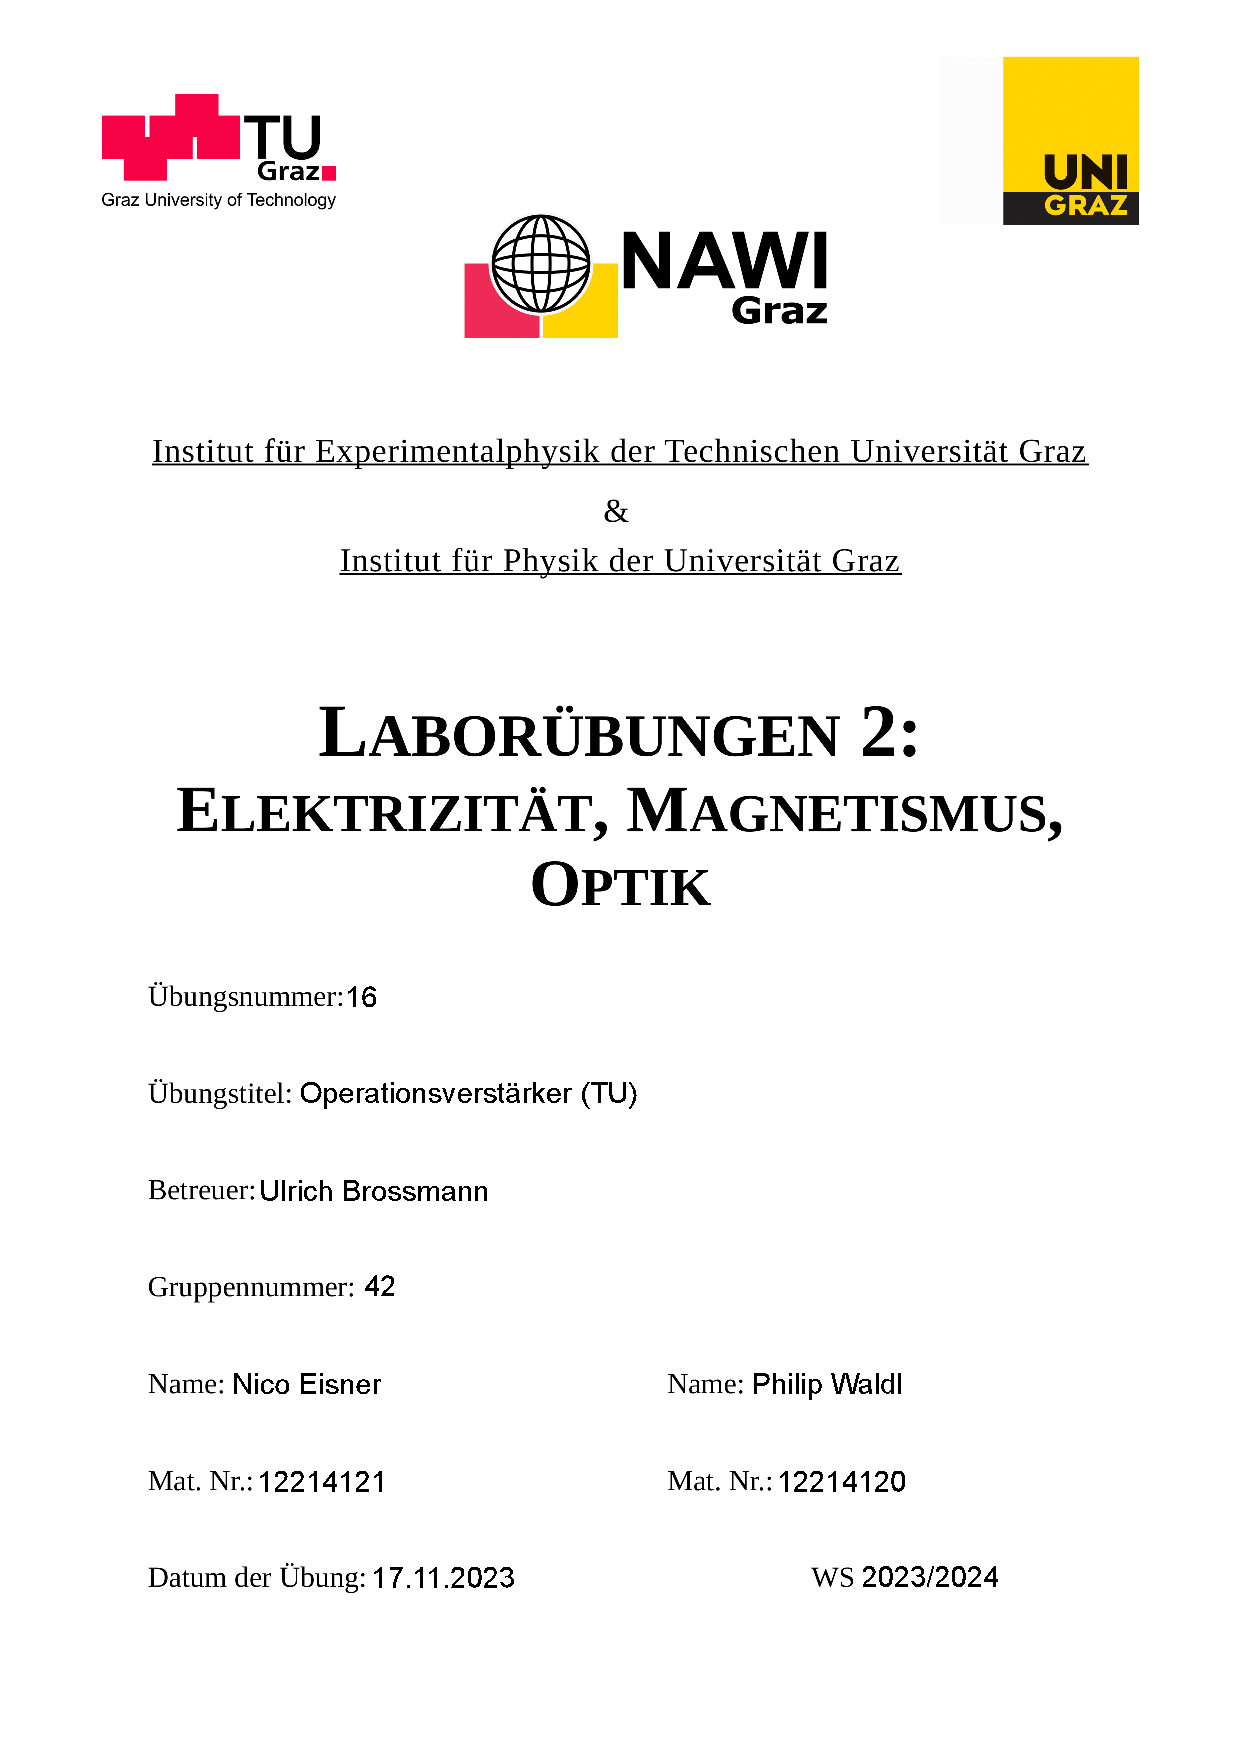
\includepdf[pages={1}]{../Deckblätter/Deckblatt_Operationsverstärker.pdf}

\tableofcontents
\newpage

\section{Aufgabenstellung} %jo beschreibn wos gmocht host ------------------------------

Der Versuche Operationsverstärker behandelt das gleichnamige Elektronikbauteil, welches in der Elektronik in erster Linie zur Verstärkung von elektrischen Signalen eingesetzt wird.
Über mehrere, verschiedene Schaltungen hinweg sollen einige Anwendungsbereiche des OPVs gezeigt und experimentell bestätigt werden.

Die genaue Aufgabenstellung sieht dabei wie folgt aus:

\begin{itemize}
    \item Aufbau der Schaltung für den Operationsverstärker (OPV)
    \item Invertierter OPV
    \begin{itemize}
        \item Verstärkung V 
        \item Phasendifferenz $\phi$ zwischen Ein- und Ausgangssingal für verschiedene Rückkopplungswiderstände $\tau$
    \end{itemize}
    \item Nichtinvertierter OPV
    \begin{itemize}
        \item Funktionsweiße des nichtinvertierten OPV für verschiedene Widerstandskombinationen
    \end{itemize}
    \item OPV als Differenzierer
    \begin{itemize}
        \item Funktionsweiße des OPV als Differenzierer für verschiedene Widerstandskombinationen und Eingangssignalarten
    \end{itemize}
    \item OPV als Integrierer
    \begin{itemize}
        \item Funktionsweiße des OPV als Integrierer für verschiedene Widerstandskombinationen und Eingangssignalarten
    \end{itemize}
\end{itemize}

\noindent
Alle Informationen und Methodiken wurden uns von der Technischen Universität bereitgestellt \cite{teachcenter2}. 


\section{Voraussetzungen \& Grundlagen} %Grundlagen erklären, Formeln mit erklärung

Wie bereits im Kapitel Aufgabenstellung eingeleitet ist der Operationsverstärker ein elektrisches Schaltelement, genauer ein gleichspannungsgekoppelter Differenzenverstärker, welcher einen invertierten- und einen nichtinvertierten Eingang besitzt. Er soll dabei die Differenz zwischen den beiden Eingangssignalen verstärken und einem idealen Verstärker (möglichst hohe Verstärkung, Eingangswiderstände und möglichst geringe Ausgangswiderstände) nahe kommen. Der grobe Aufbau eines OPVs lässt sich in folgender Abbildung \ref{fig:OpvAufbau} erkennen.

\begin{figure}[H]
    \centering
    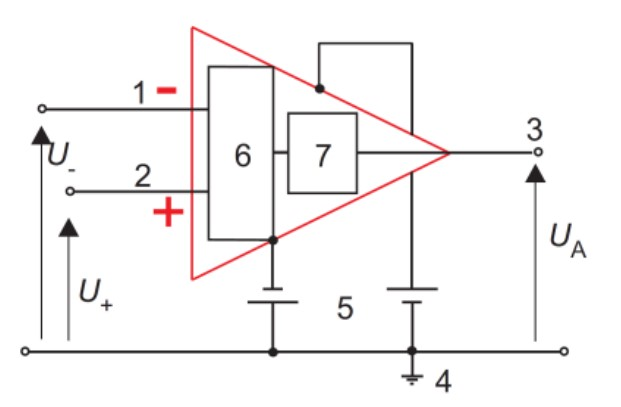
\includegraphics[width=0.6\linewidth]{nudes/OpvGrundlegenderAufbau.jpg}
    \caption{OPV grundlegender Aufbau \cite{teachcenter2}}
    \label{fig:OpvAufbau}
\end{figure}

\noindent
In Abbildung \ref{fig:OpvAufbau} lassen sich die beiden Eingänge 1 (invertiert) und 2 (nicht invertiert) und der Ausgang 3 erkennen. Weiters befindet sich im OPV (meist dargestellt als Dreieck) ein Differenzenverstärker 6 und ein Impedanzwandler 7. Für den Betrieb ist außerdem eine Spannungsversorgung 5 und ein gemeinsamer Groundpunkt 4 von nöten. \newline

\noindent
Die Verstärkung eines OPV wird oft auch in Dezibel angegeben, wofür folgende Formel zur Umrechnung verwendet wurde:

\begin{equation}
    \label{eq:VerstärkungDezibel}
    \centerline{$V_{L} = 20*log(\frac{U_{2}}{U_{1}}) = 20*log(V)$ \\ $\Delta V_{L} = \vert \frac{\partial V_{L}}{\partial V} * \Delta V \vert$}
\end{equation}

\noindent
Mit dem beschriebenen Operationsverstärker lassen sich nun einige Grundschaltungen darstellen:

\subsection{Invertierender Verstärker}

Beim invertierenden Verstärker wird das Signal über den invertierten Eingang mit einem Eingagnswiderstand $R_{1}$ eingespeist und der nichtinvertierte Eingang ist auf Ground gelegt. Der Widerstand $R_{2}$ ist dabei der Rückkopplungswiderstand, welcher bestimmt, wie viel vom Ausgangssignal zurück zum Eingang fließt und das Signal verstärkt.
Das Resultat des invertierten Verstärkers ist ein verstärktes und umgekehrtes Ausgangssignal, welches vom Verhältnis der beiden Widerstände abhänge und sich somit folgend beschreiben lässt:

\begin{equation}
    \label{eq:InvertierenderVerstärkerAusgang}
    \centerline{$U_{A}=-\frac{R_{2}}{R_{1}}U_{1}$}
\end{equation}

\noindent
Die Verstärkung lässt sich dabei so ausdrücken:

\begin{equation}
    \label{eq:InvertierenderVerstärkerVerstärkung}
    \centerline{$V=-\frac{R_{2}}{R_{1}} = -\frac{U_{Aus}}{U_{Ein}}$ \\ $\Delta V = \vert \frac{\partial V}{\partial U_{Aus}} * \Delta U_{Aus} \vert + \vert \frac{\partial V}{\partial U_{Ein}} * \Delta U_{Ein} \vert $}
\end{equation}

\noindent
Das Schaltbild des invertierten Verstärkers lässt sich in folgender Abbildung \ref{fig:InvertierenderVerstärker} erkennen.

\begin{figure}[H]
    \centering
    \includegraphics[width=0.3\linewidth]{nudes/Invertierender Verstärker.jpg}
    \caption{Invertierender Verstärker \cite{teachcenter2}}
    \label{fig:InvertierenderVerstärker}
\end{figure}


\subsection{Nichtinvertierender Verstärker}

Der nichtinvertierende Verstärker sieht im Aufbau dem invertierenden Verstärker sehr ähnlich. Der größte Unterschied ist, dass das Eingangssignal über den nichtinvertierten Eingang mit Eingagnswiderstand kommt und der invertierte Eingang auf Masse gelegt ist.
Beim nichtinvertierenden Verstärker verlässt das Signal die Schaltung nur verstärkt, was in folgender Gleichung für die Verstärkung resultiert:

\begin{equation}
    \label{eq:NichtinvertierenderVerstärkerVerstärkung}
    \centerline{$V=1 + \frac{R_{2}}{R_{1}} = \frac{U_{A}}{U_{E}}$  \\ $\Delta V = \vert \frac{\partial V}{\partial U_{Aus}} * \Delta U_{Aus} \vert + \vert \frac{\partial V}{\partial U_{Ein}} * \Delta U_{Ein} \vert $}
\end{equation}

\noindent
Der Aufbau sieht dabei wie folgt aus:

\begin{figure}[H]
    \centering
    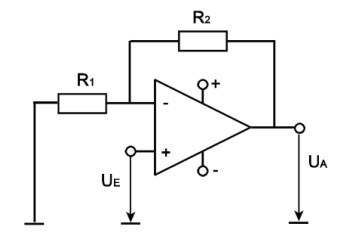
\includegraphics[width=0.3\linewidth]{nudes/Nichtinvertierender Verstärker.jpg}
    \caption{Nichtinvertierender Verstärker \cite{teachcenter2}}
    \label{fig:NichtInvertierenderVerstärker}
\end{figure}


\subsection{Addierer, Subtrahierer}

Werden zwei Eingangsspannungen mit Eingangswiderständen an den invertierten Eingang- und eine Eingangsspannung mit Spannungsteiler an den nichtinvertierten Eingang geschaltet, so erhält man einen funktionstüchtigen Addierer bzw. Subtrahierer.
Die Funktion der Schaltung ist dabei von den gewählten Widerständen abhängig und sieht im Aufbau wie folgt aus:

\begin{figure}[H]
    \centering
    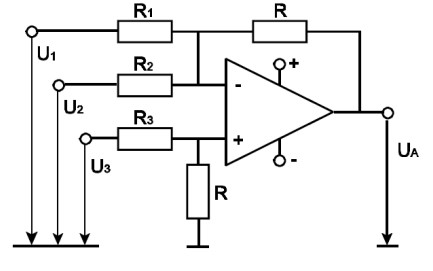
\includegraphics[width=0.3\linewidth]{nudes/AddiererSubtrahierer.jpg}
    \caption{Addierer/Subtrahierer \cite{teachcenter2}}
    \label{fig:AddiererSubtrahierer}
\end{figure}


\subsection{Differenzierer}

Des weiteren ist es möglich, unter einbezug eines Operationsverstärkers zu differenzieren. Dabei wird der invertierenden Verstärkerschaltung ein Kondensator vor dem Eingangswiderstand $R_{1}$ hinzugefügt. Anhand der Lade- bzw. Entladezeiten lässt sich so durch die zeitliche Ableitung von $Q = C*U_{E}$ die Ausgangsspannung als differenzierte Eingangsspannung definieren:

\begin{equation}
    \label{eq:DifferenziererAusgang}
    \centerline{$U_{A}=-RC \frac{\partial U_{E}}{\partial t}$}
\end{equation}

\noindent
Die hierzu nötige Schaltung ist in Abbildung \ref{fig:Integrierer} ersichtlich.

\begin{figure}[H]
    \centering
    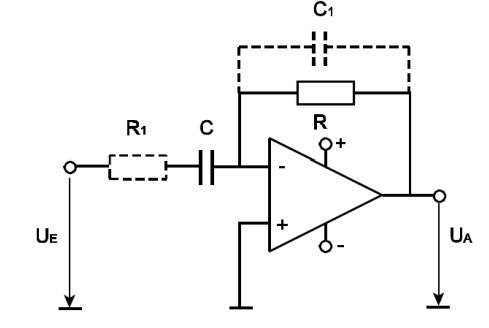
\includegraphics[width=0.3\linewidth]{nudes/Differenzierer.jpg}
    \caption{Differenzierer \cite{teachcenter2}}
    \label{fig:Differenzierer}
\end{figure}


\subsection{Integrierer}

Ähnlichem Prinzip folgt auch der Integrierer, welcher sich zum Differenzierer lediglich durch die Anordnung des Kondensators unterscheidet. Dieser wird nun nicht vor den Eingangswiderstand, sondern paralell zum Rückkopplungswiderstand geschaltet.
Dadurch erzielt man an der Ausgangsspannung die Stammfunktion der Eingangsspannung.

\begin{equation}
    \label{eq:IntegriererAusgang}
    \centerline{$U_{A}=-\frac{1}{RC} \int_{}^{} U_{E} \,dt + c $}
\end{equation}

\noindent
Aufgebaut sieht der Integrierer wie folgt aus:

\begin{figure}[H]
    \centering
    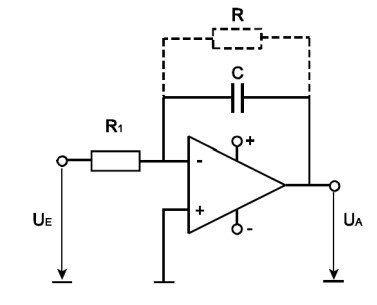
\includegraphics[width=0.3\linewidth]{nudes/Integrierer.jpg}
    \caption{Integrierer \cite{teachcenter2}}
    \label{fig:Integrierer}
\end{figure}


\section{Versuchsanordnung} %mit skizze kurz beschreiben ------------------------------

Zu Beginn des Versuches wurden zwei grundlegende Schaltungen realisiert, welche abgesehen vom Operationsverstärker noch ein bzw. zwei Potentiometer mit 100 $\Omega$, zwei Widerstände mit 47 $k \Omega$, den Funktionsgenerator und das Netzgerät mit einer Spannnung von $\pm$15 V. Der Aufbau der Schaltung ist in folgenden Abbildungen \ref{fig:GrundschaltungAufbau} ersichtlich.

\begin{figure}[H]
    \centering
    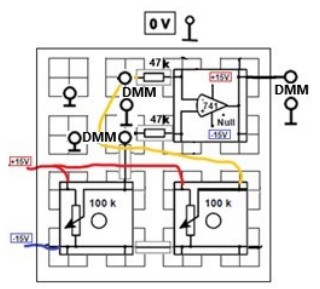
\includegraphics[width=0.4\linewidth]{nudes/GrundschaltungAufbau1.jpg}
    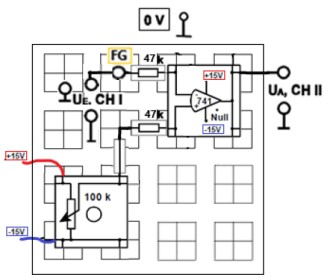
\includegraphics[width=0.4\linewidth]{nudes/GrundschaltungAufbau2.jpg}
    \caption{Grundschaltungen Aufbau \cite{teachcenter2}}
    \label{fig:GrundschaltungenAufbau}
\end{figure}

\begin{figure}[H]
    \centering
    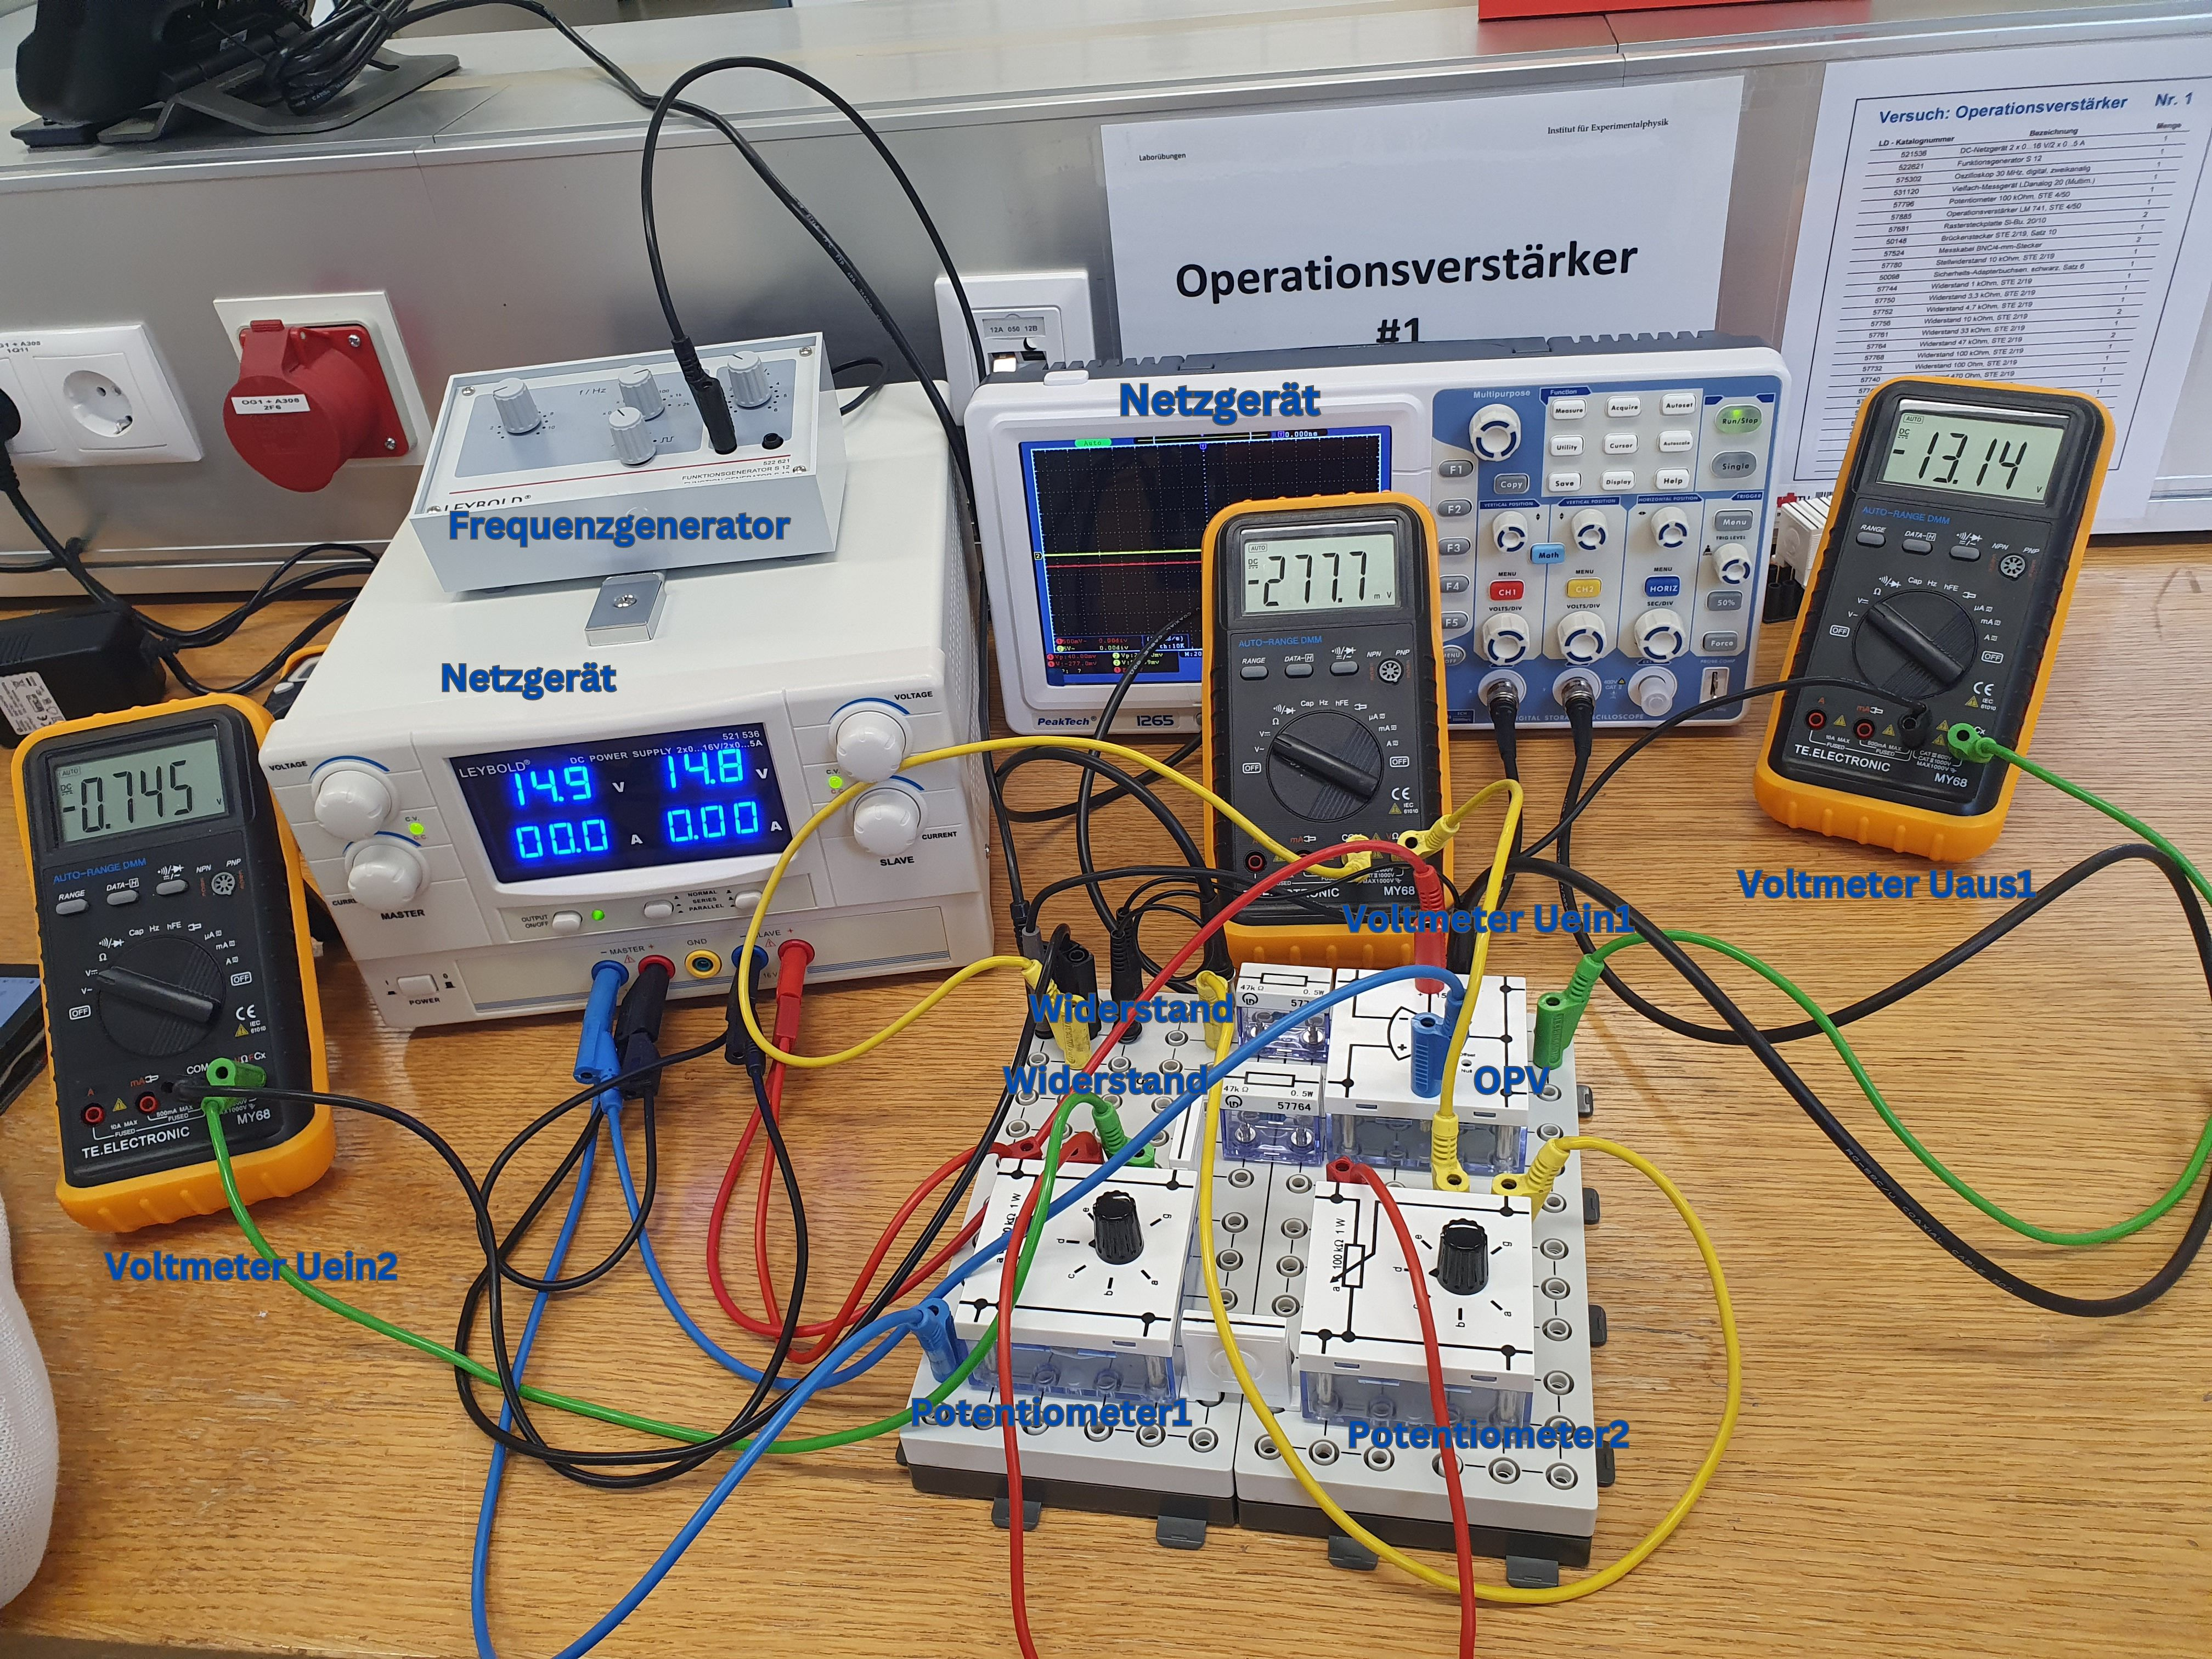
\includegraphics[width=0.4\linewidth]{nudes/messergebnisse/GrundschaltungIRL1.jpg}
    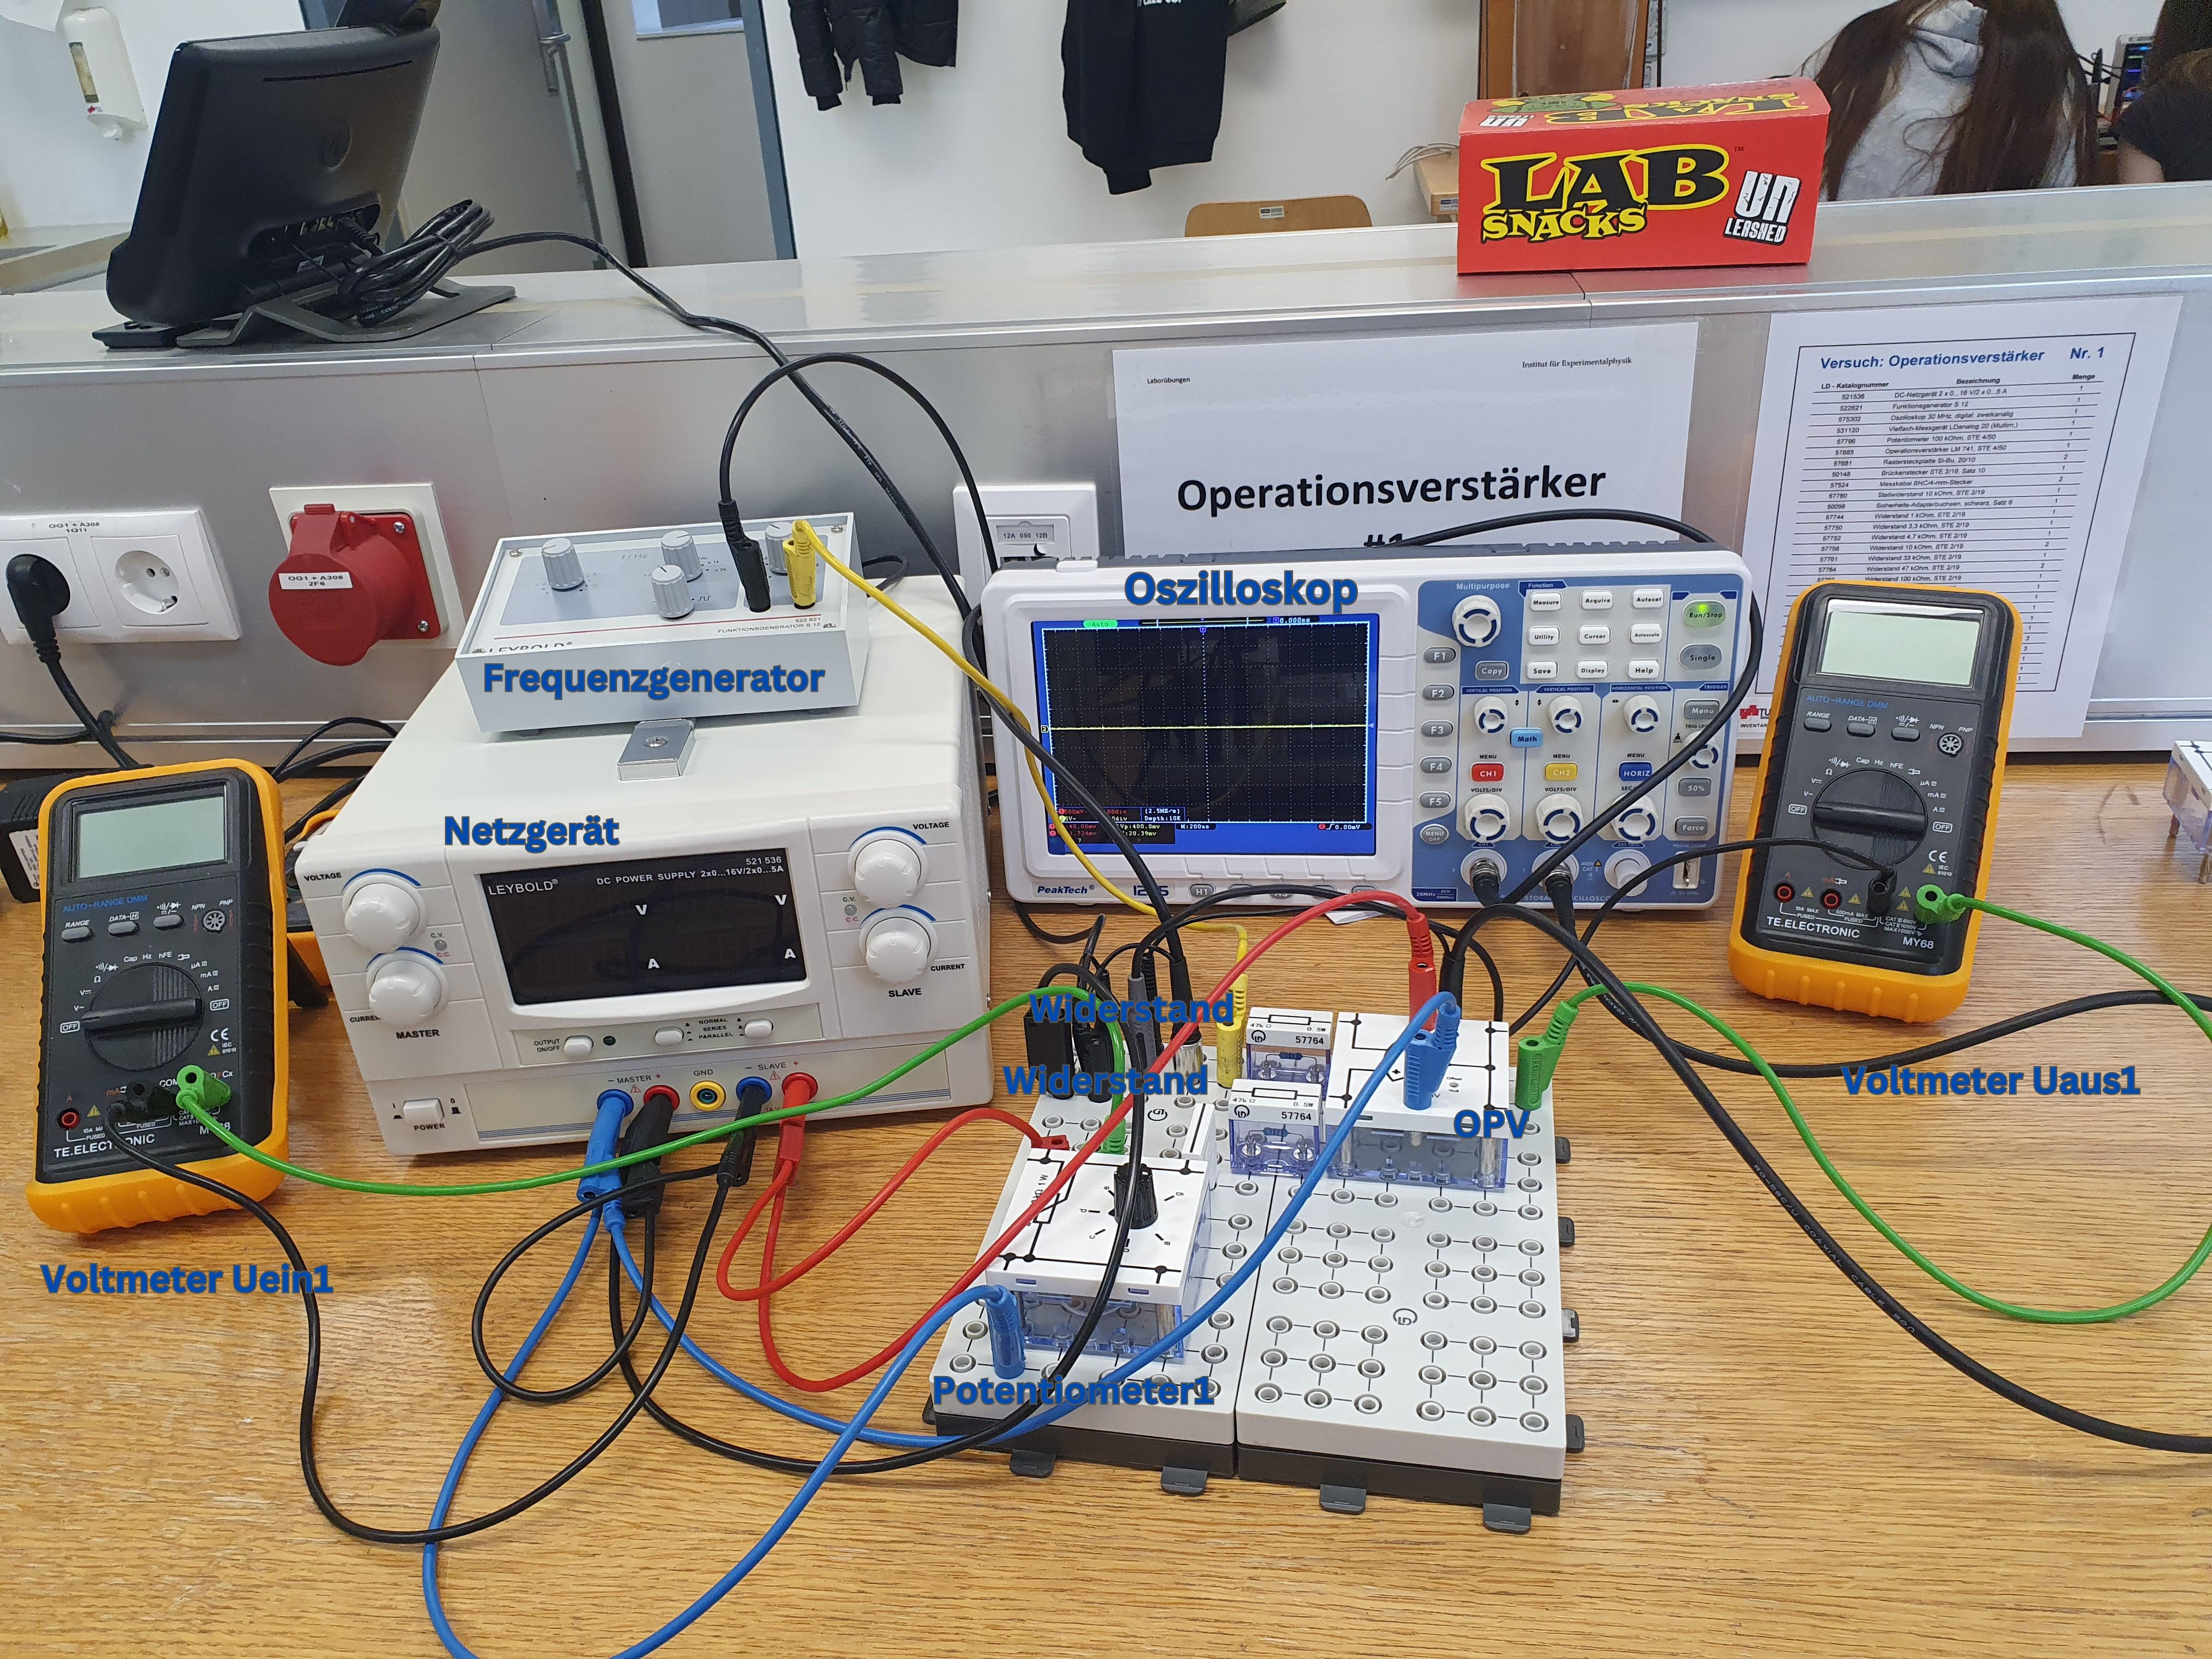
\includegraphics[width=0.4\linewidth]{nudes/messergebnisse/GrundschaltungIRL2.jpg}
    \caption{Grundschaltungen realer Aufbau}
    \label{fig:GrundschaltungenAufbauIRL}
\end{figure}

\noindent
Folgend dazu wurde dann der invertierende Verstärker realisiert. Der Schaltungsaufbau hierzu ist in folgenden Abbildungen zu erkennen.

\begin{figure}[H]
    \centering
    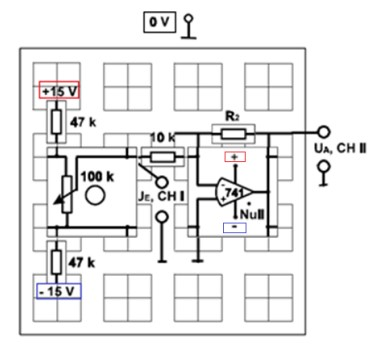
\includegraphics[width=0.4\linewidth]{nudes/InvertierenderVerstärkerSchaltungAufbau.jpg}
    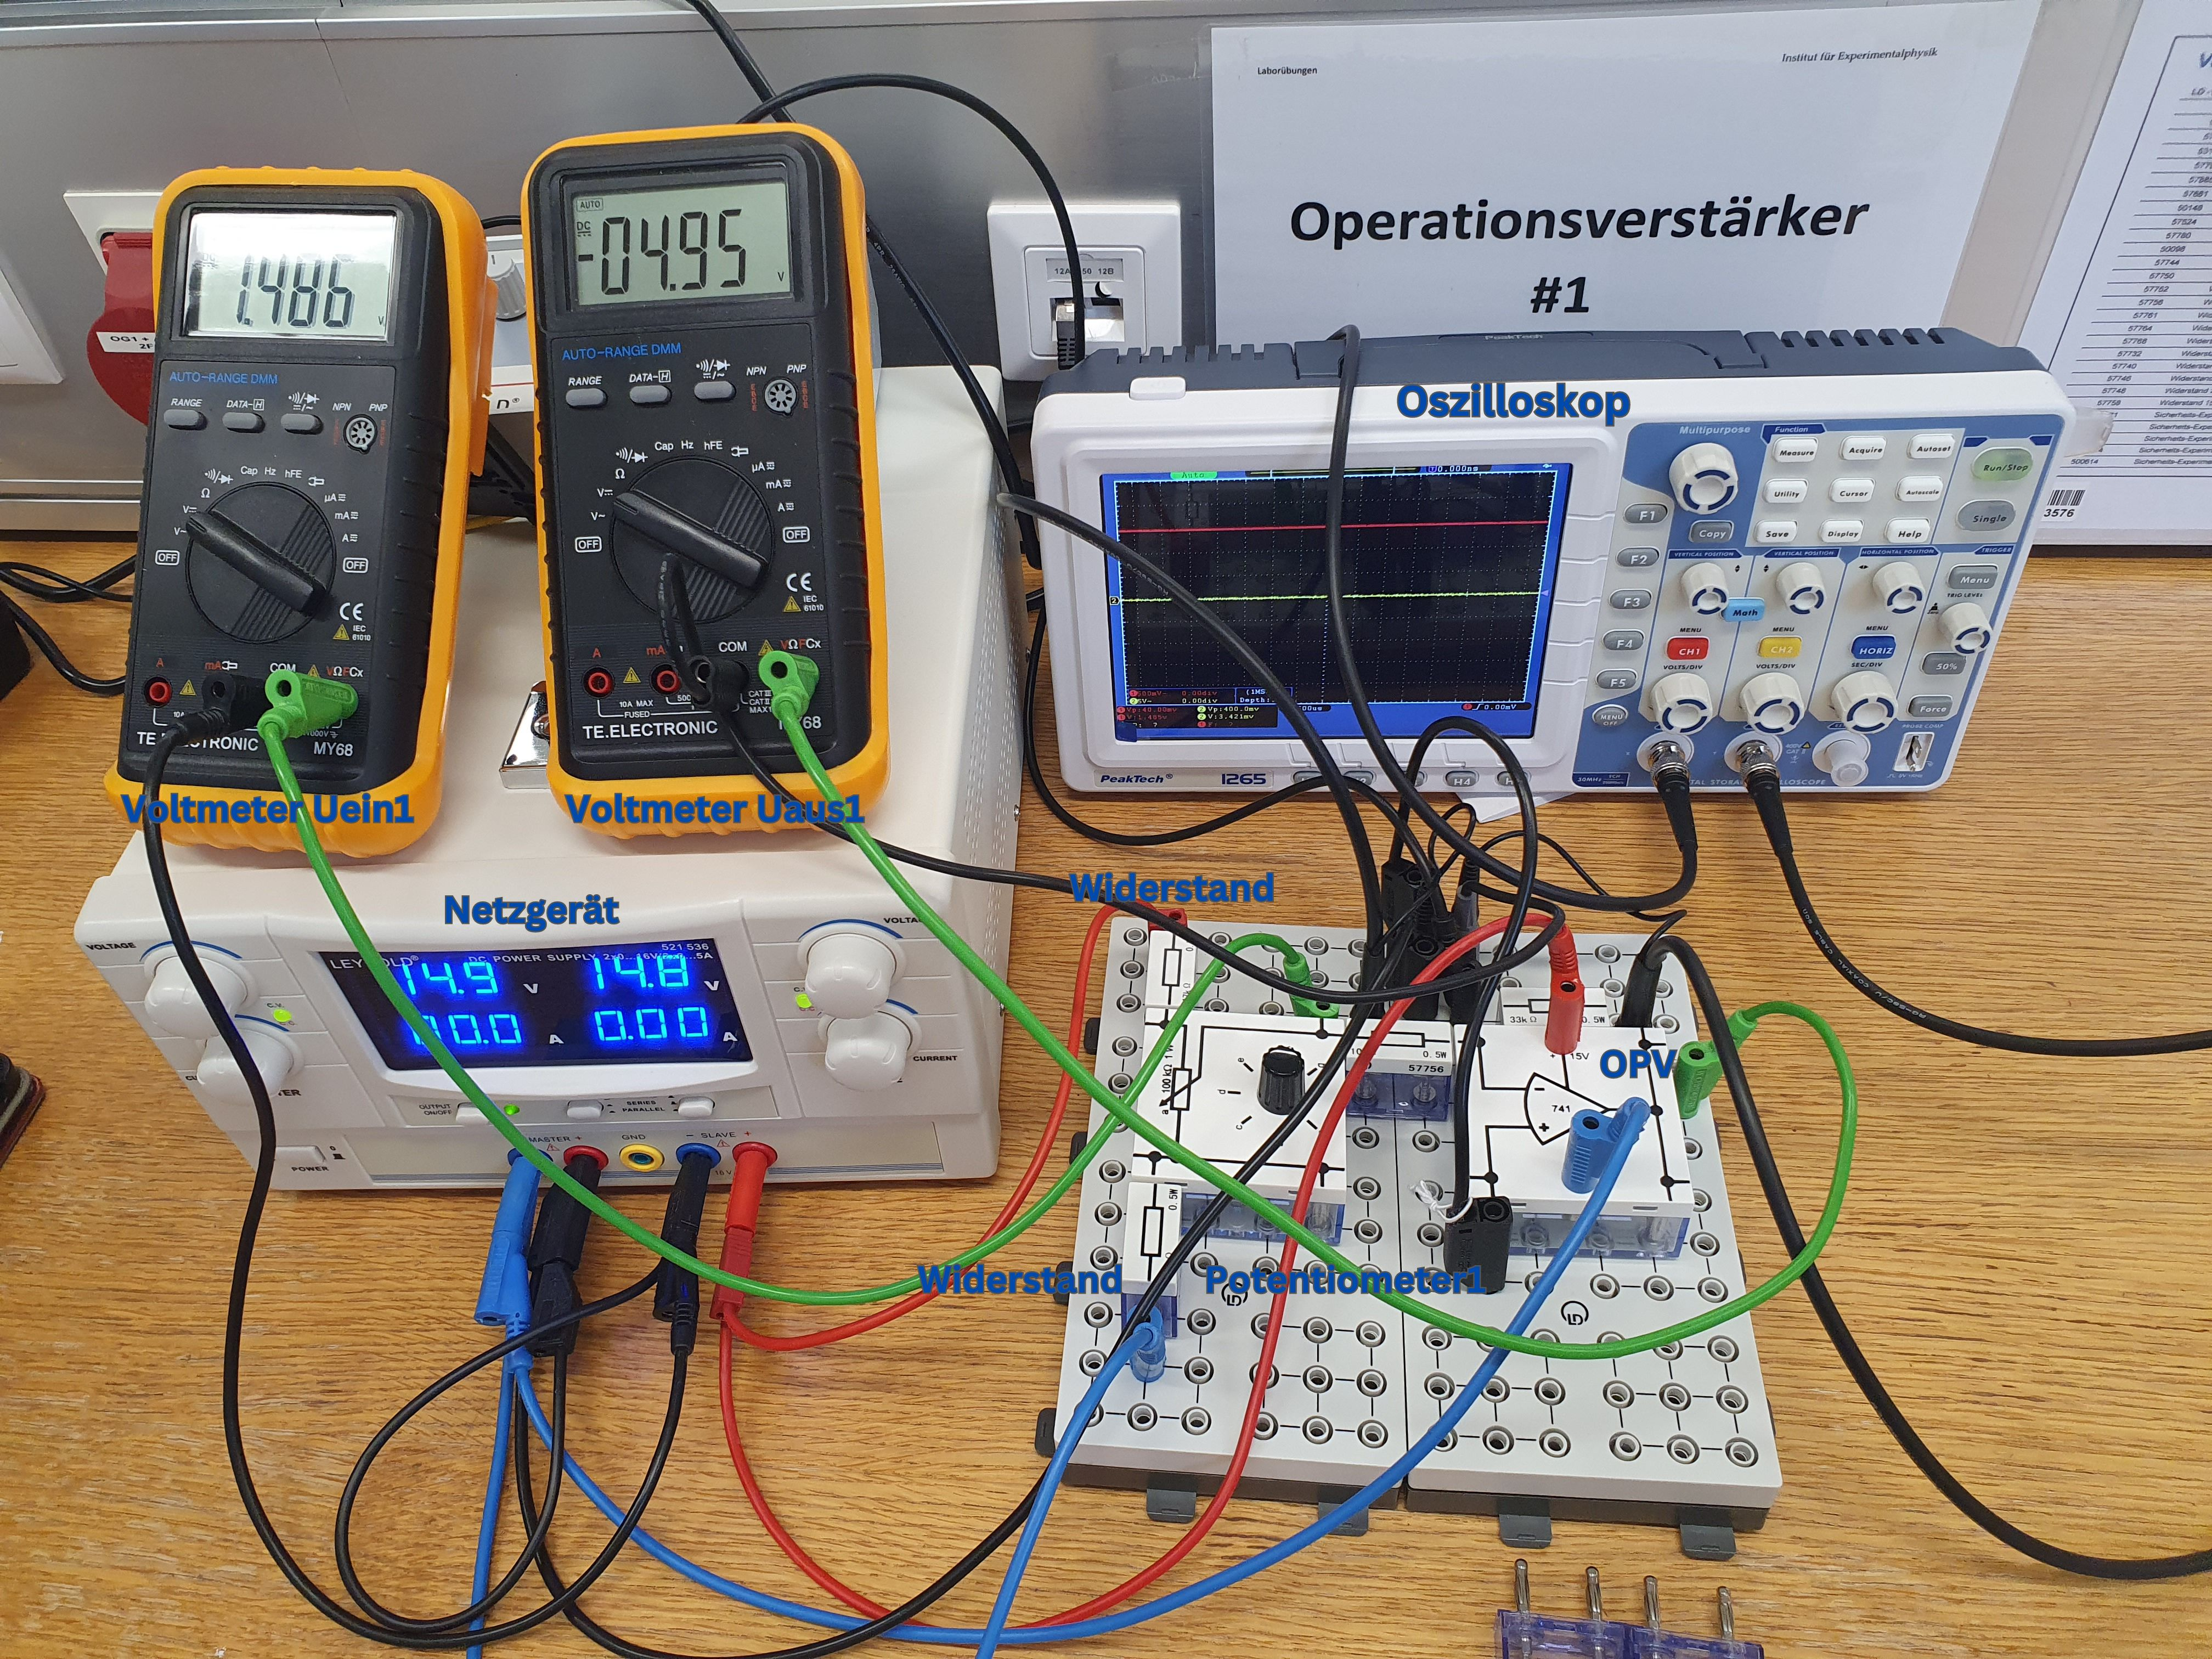
\includegraphics[width=0.4\linewidth]{nudes/messergebnisse/InvertierenderVerstIRL.jpg}
    \caption{Invertierender Verstärker Schaltung und realer Aufbau \cite{teachcenter2}}
    \label{fig:SchaltungInvertierenderVerstärker}
\end{figure}

\noindent
Natürlich wurde dann auch der nichtinvertierende Verstärker in Realität umgesetzt:

\begin{figure}[H]
    \centering
    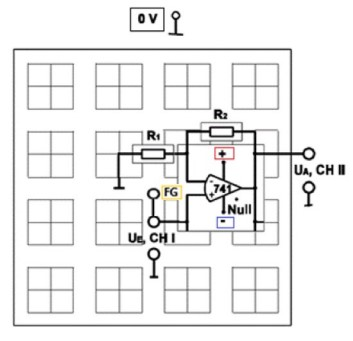
\includegraphics[width=0.4\linewidth]{nudes/NichtInvertierenderVerstärkerSchaltungAufbau.jpg}
    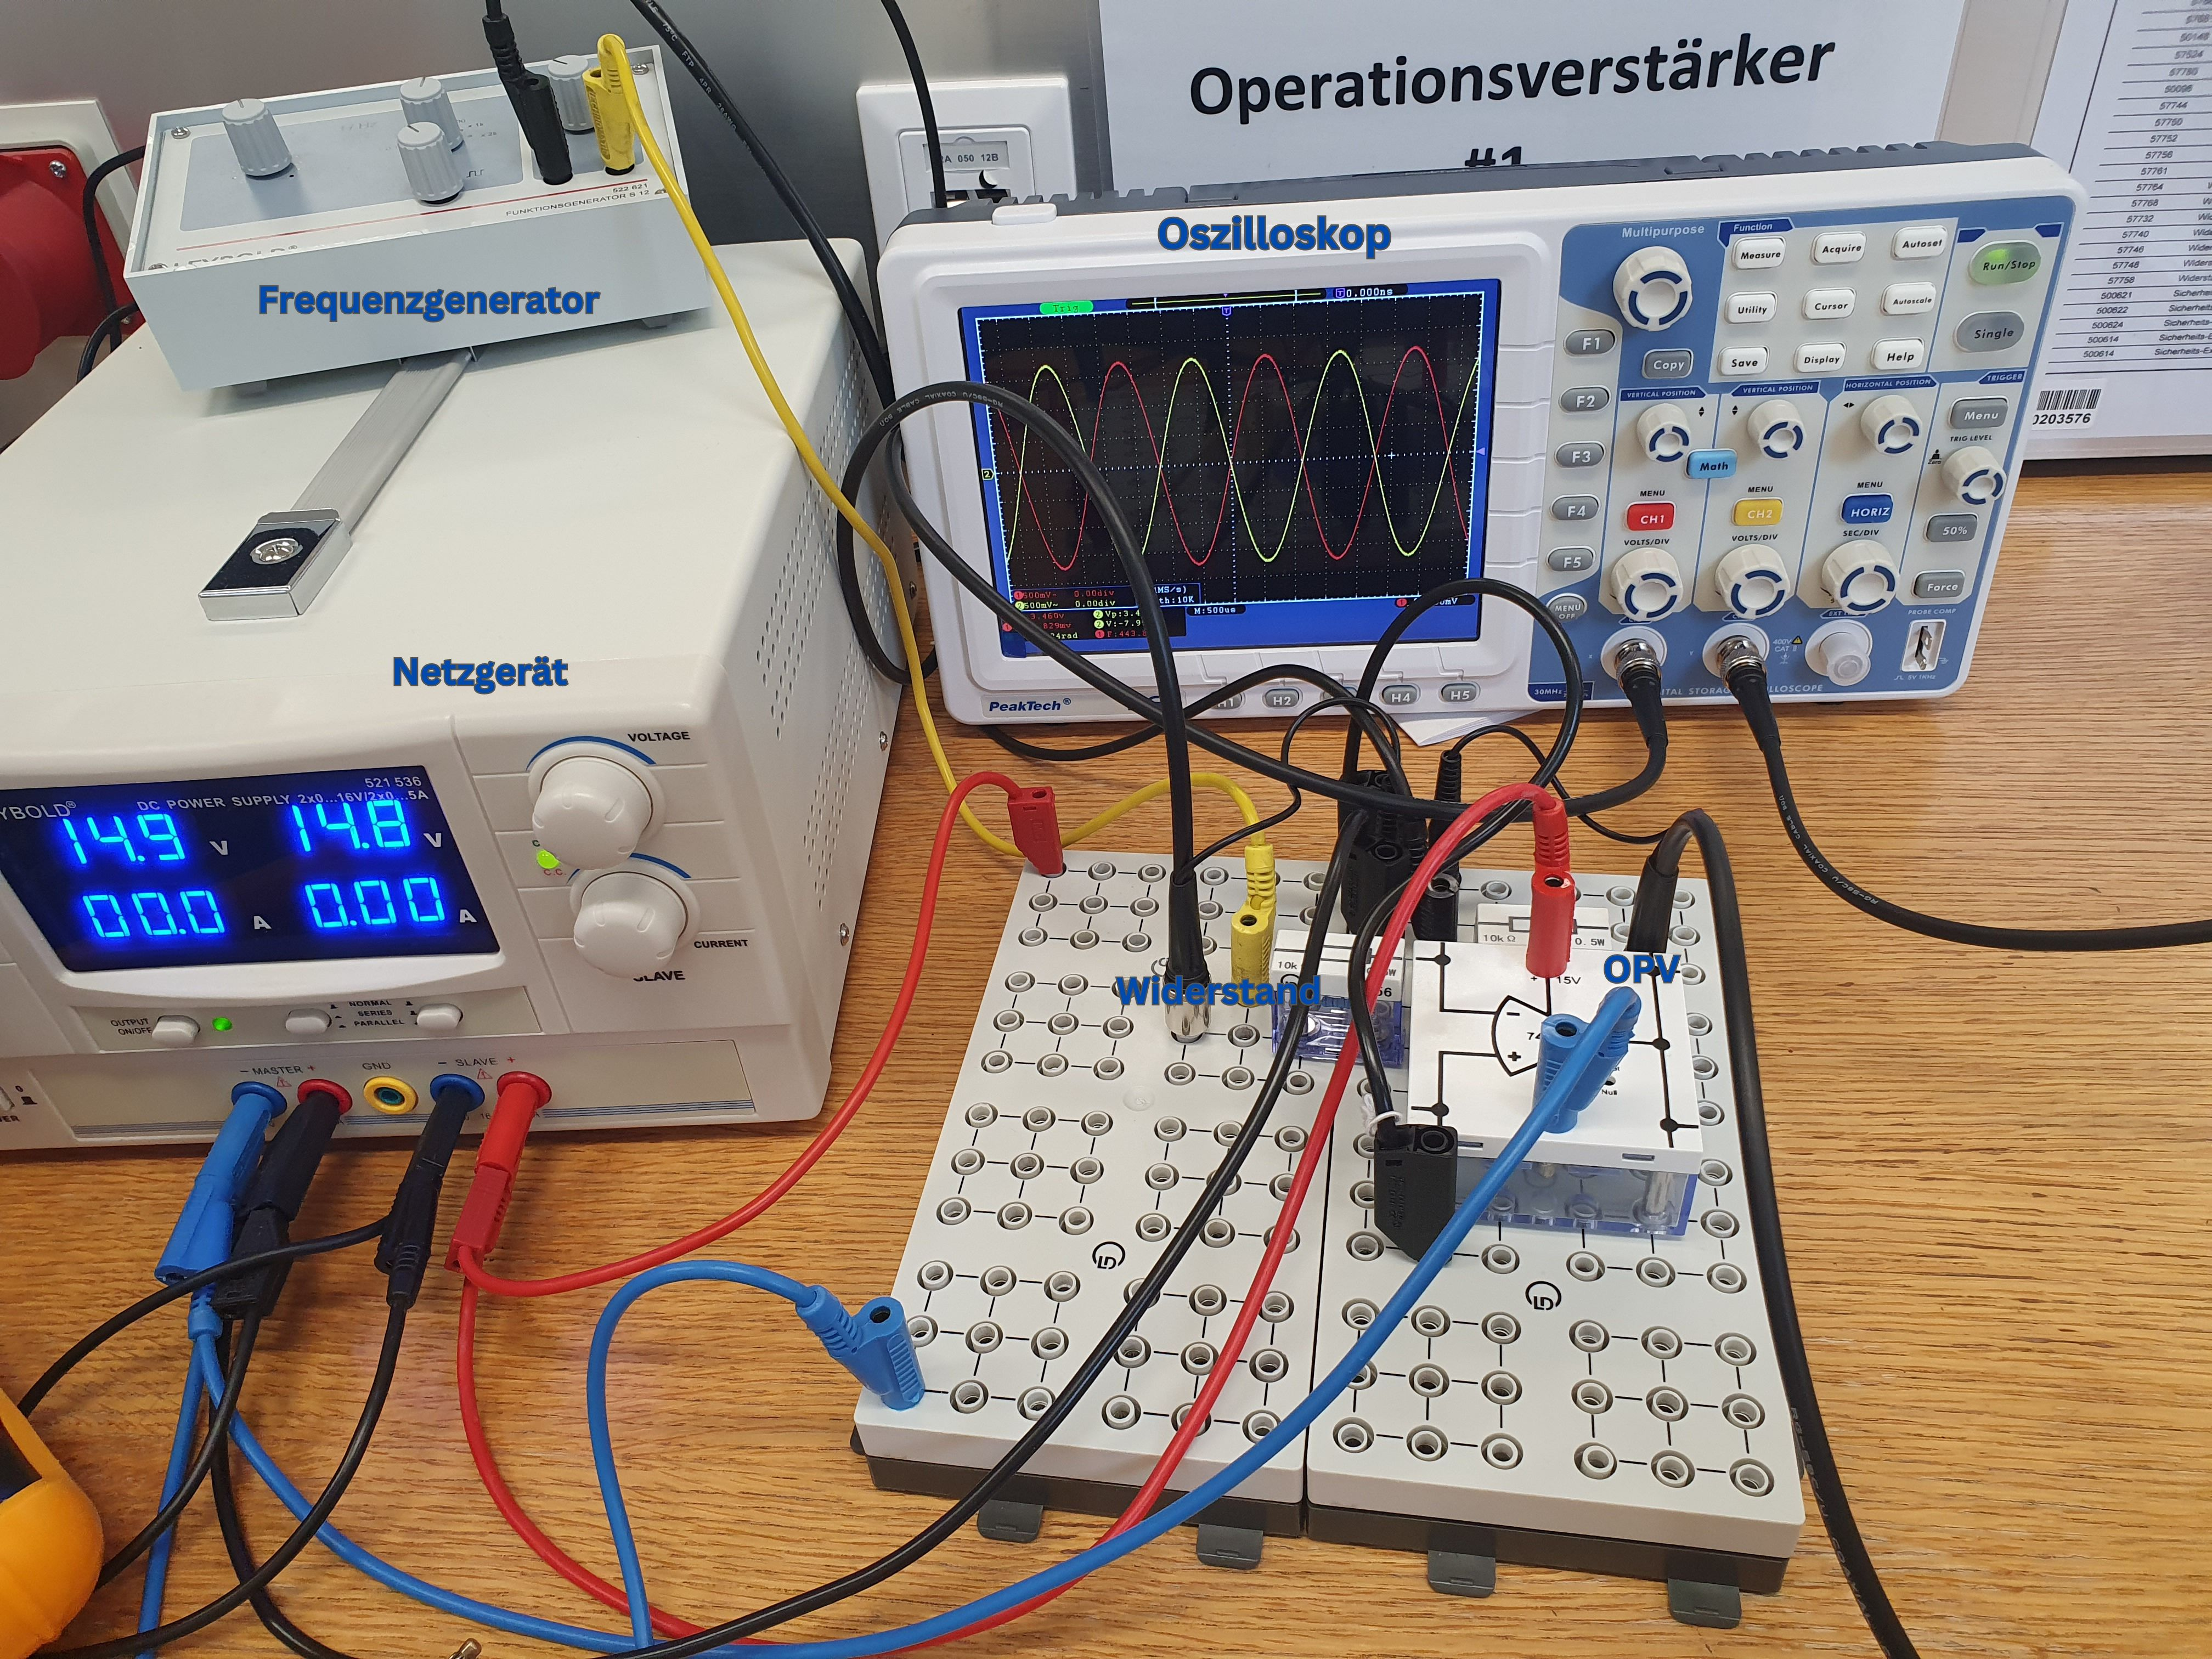
\includegraphics[width=0.4\linewidth]{nudes/messergebnisse/NichtinvertierenderIRL.jpg}
    \caption{Nichtinvertierender Verstärker Schaltung und realer Aufbau \cite{teachcenter2}}
    \label{fig:SchaltungNichtInvertierenderVerstärker}
\end{figure}

\noindent
Am Ende des Versuches wurde es dann etwas komplexer, da nun Differenzierer und Integrierer in die Tat umgesetzt wurden. Die hierfür benötigten Schaltpläne sind in folgenden Abbildungen ersichtlich: 

\begin{figure}[H]
    \centering
    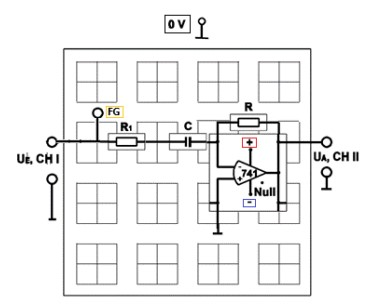
\includegraphics[width=0.4\linewidth]{nudes/DifferenziererSchaltungAufbau.jpg}
    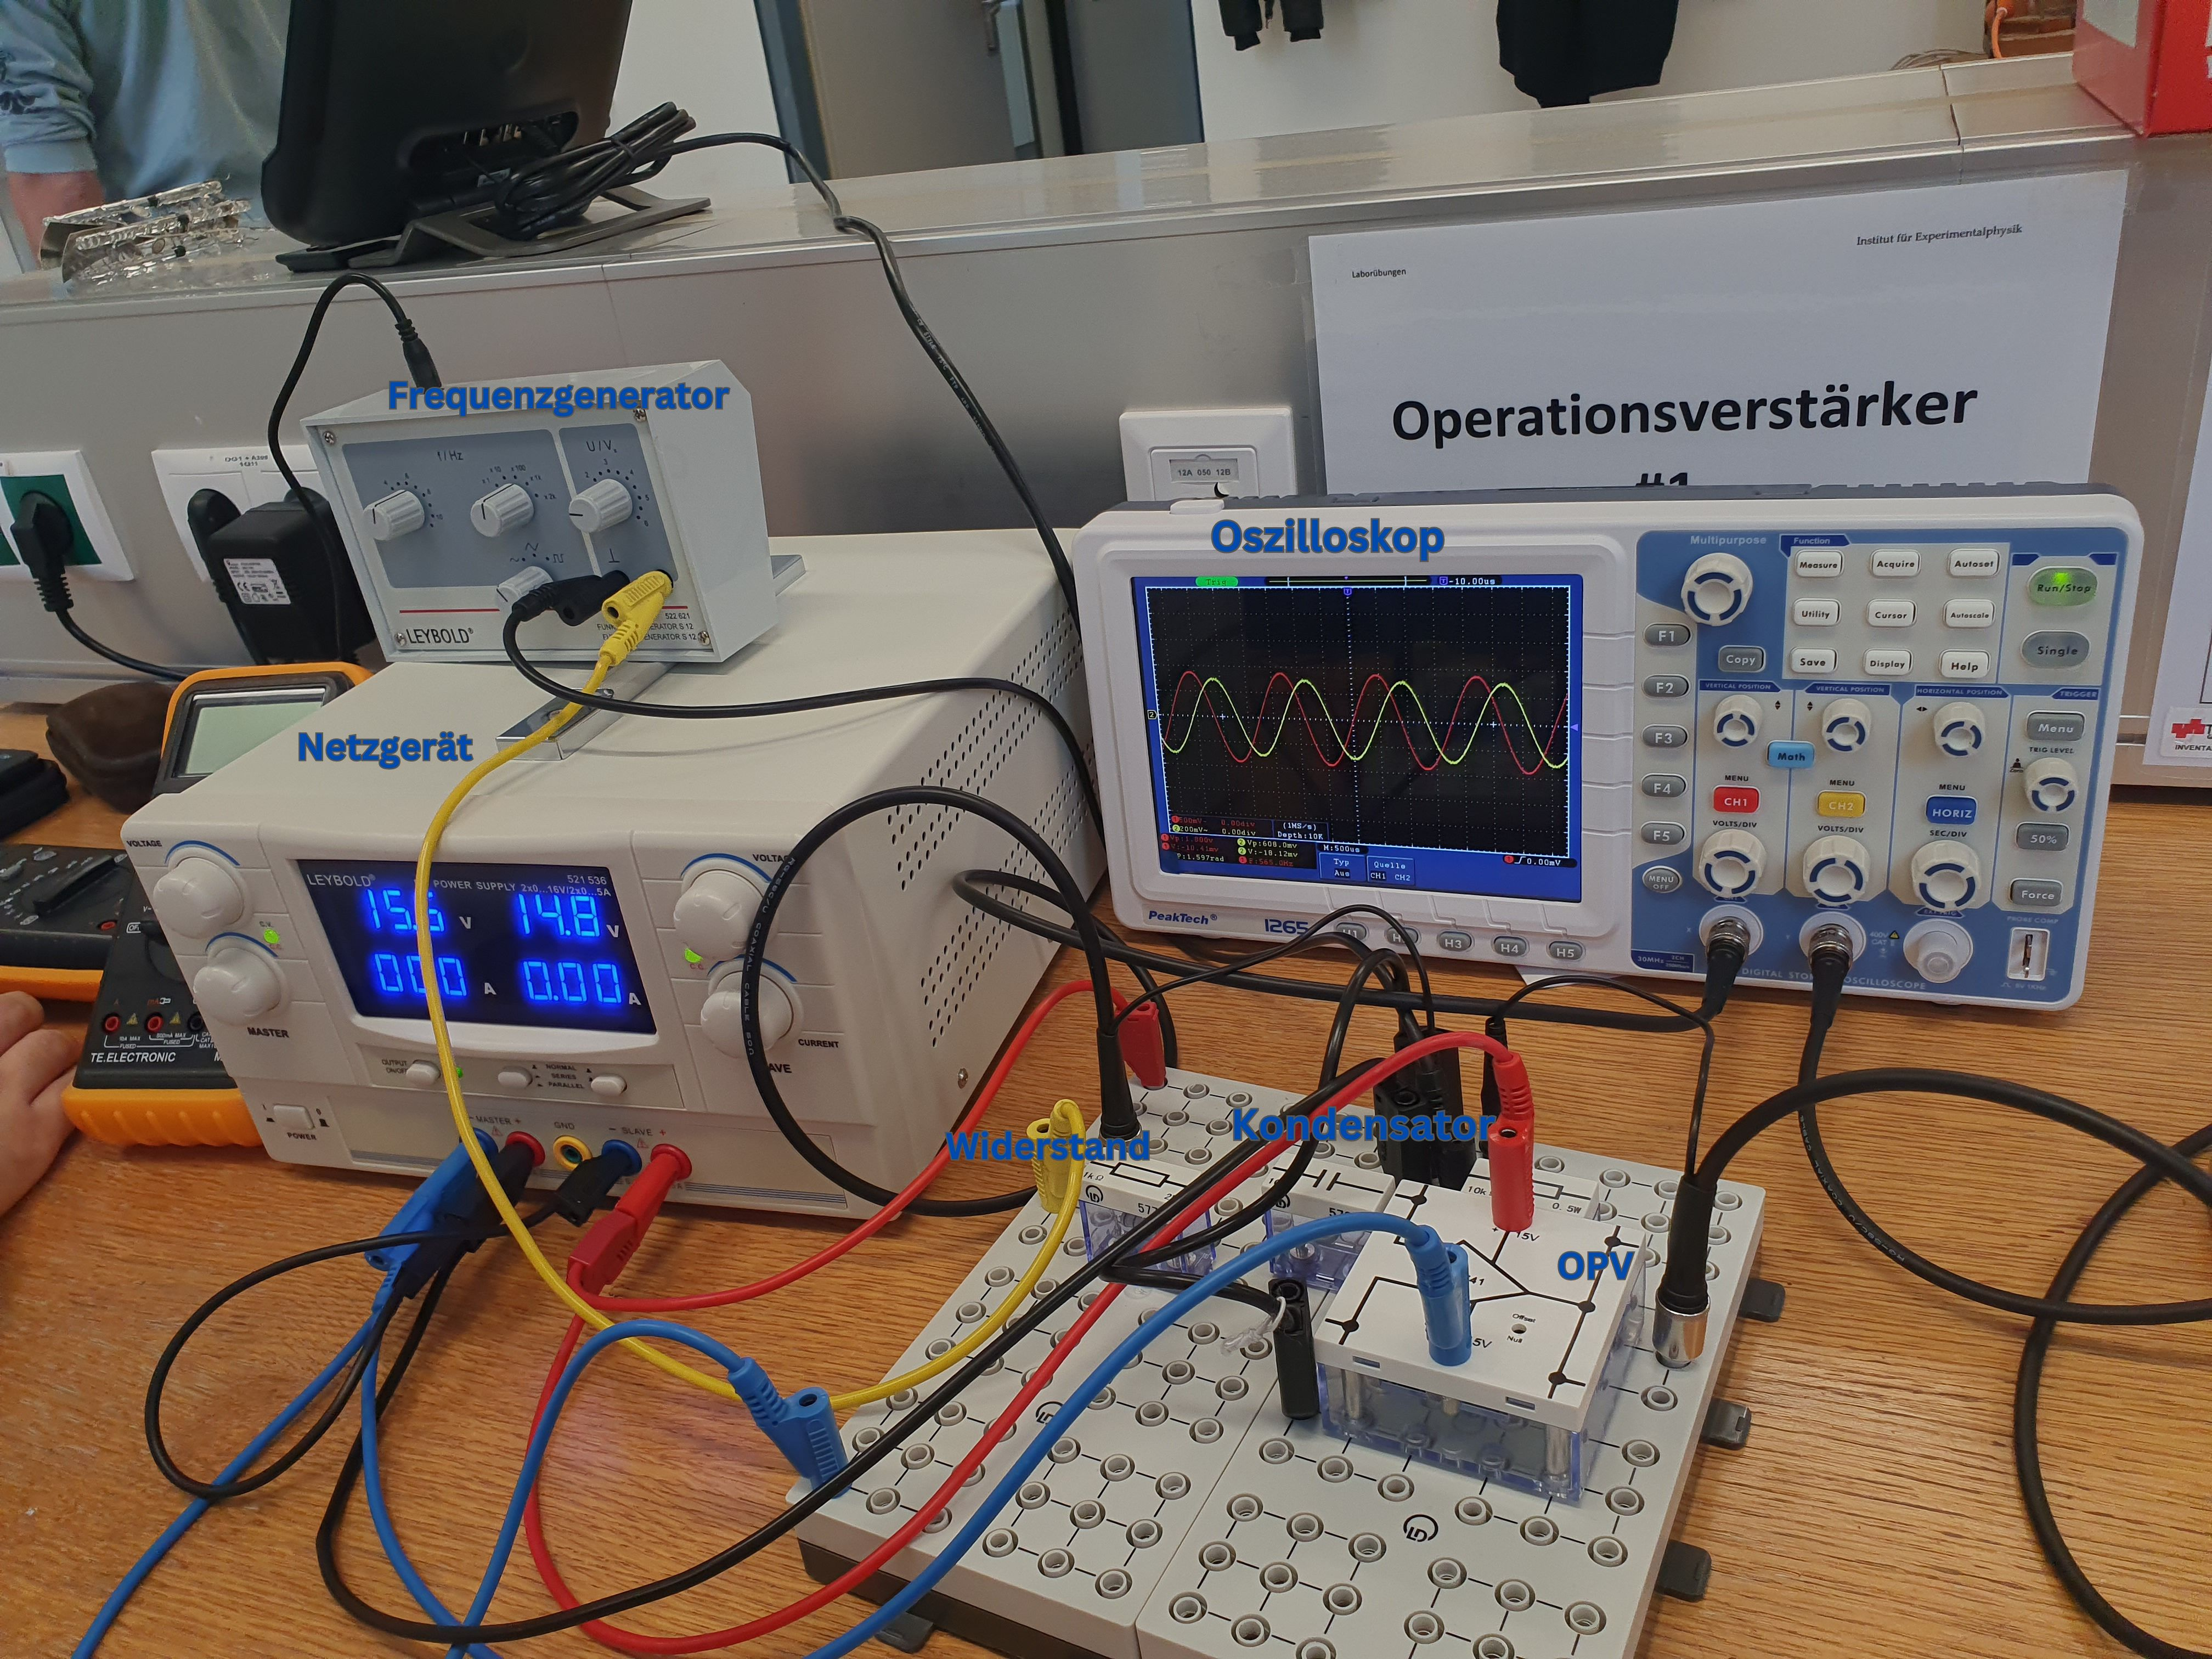
\includegraphics[width=0.4\linewidth]{nudes/messergebnisse/DifferenziererIRL.jpg}
    \caption{Differenzierer Schaltung und realer Aufbau \cite{teachcenter2}}
    \label{fig:SchaltungDifferenzierer}
\end{figure}

\begin{figure}[H]
    \centering
    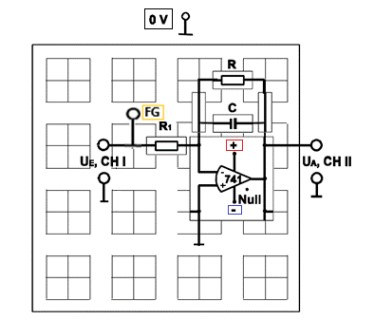
\includegraphics[width=0.4\linewidth]{nudes/IntegriererSchaltungAufbau.jpg}
    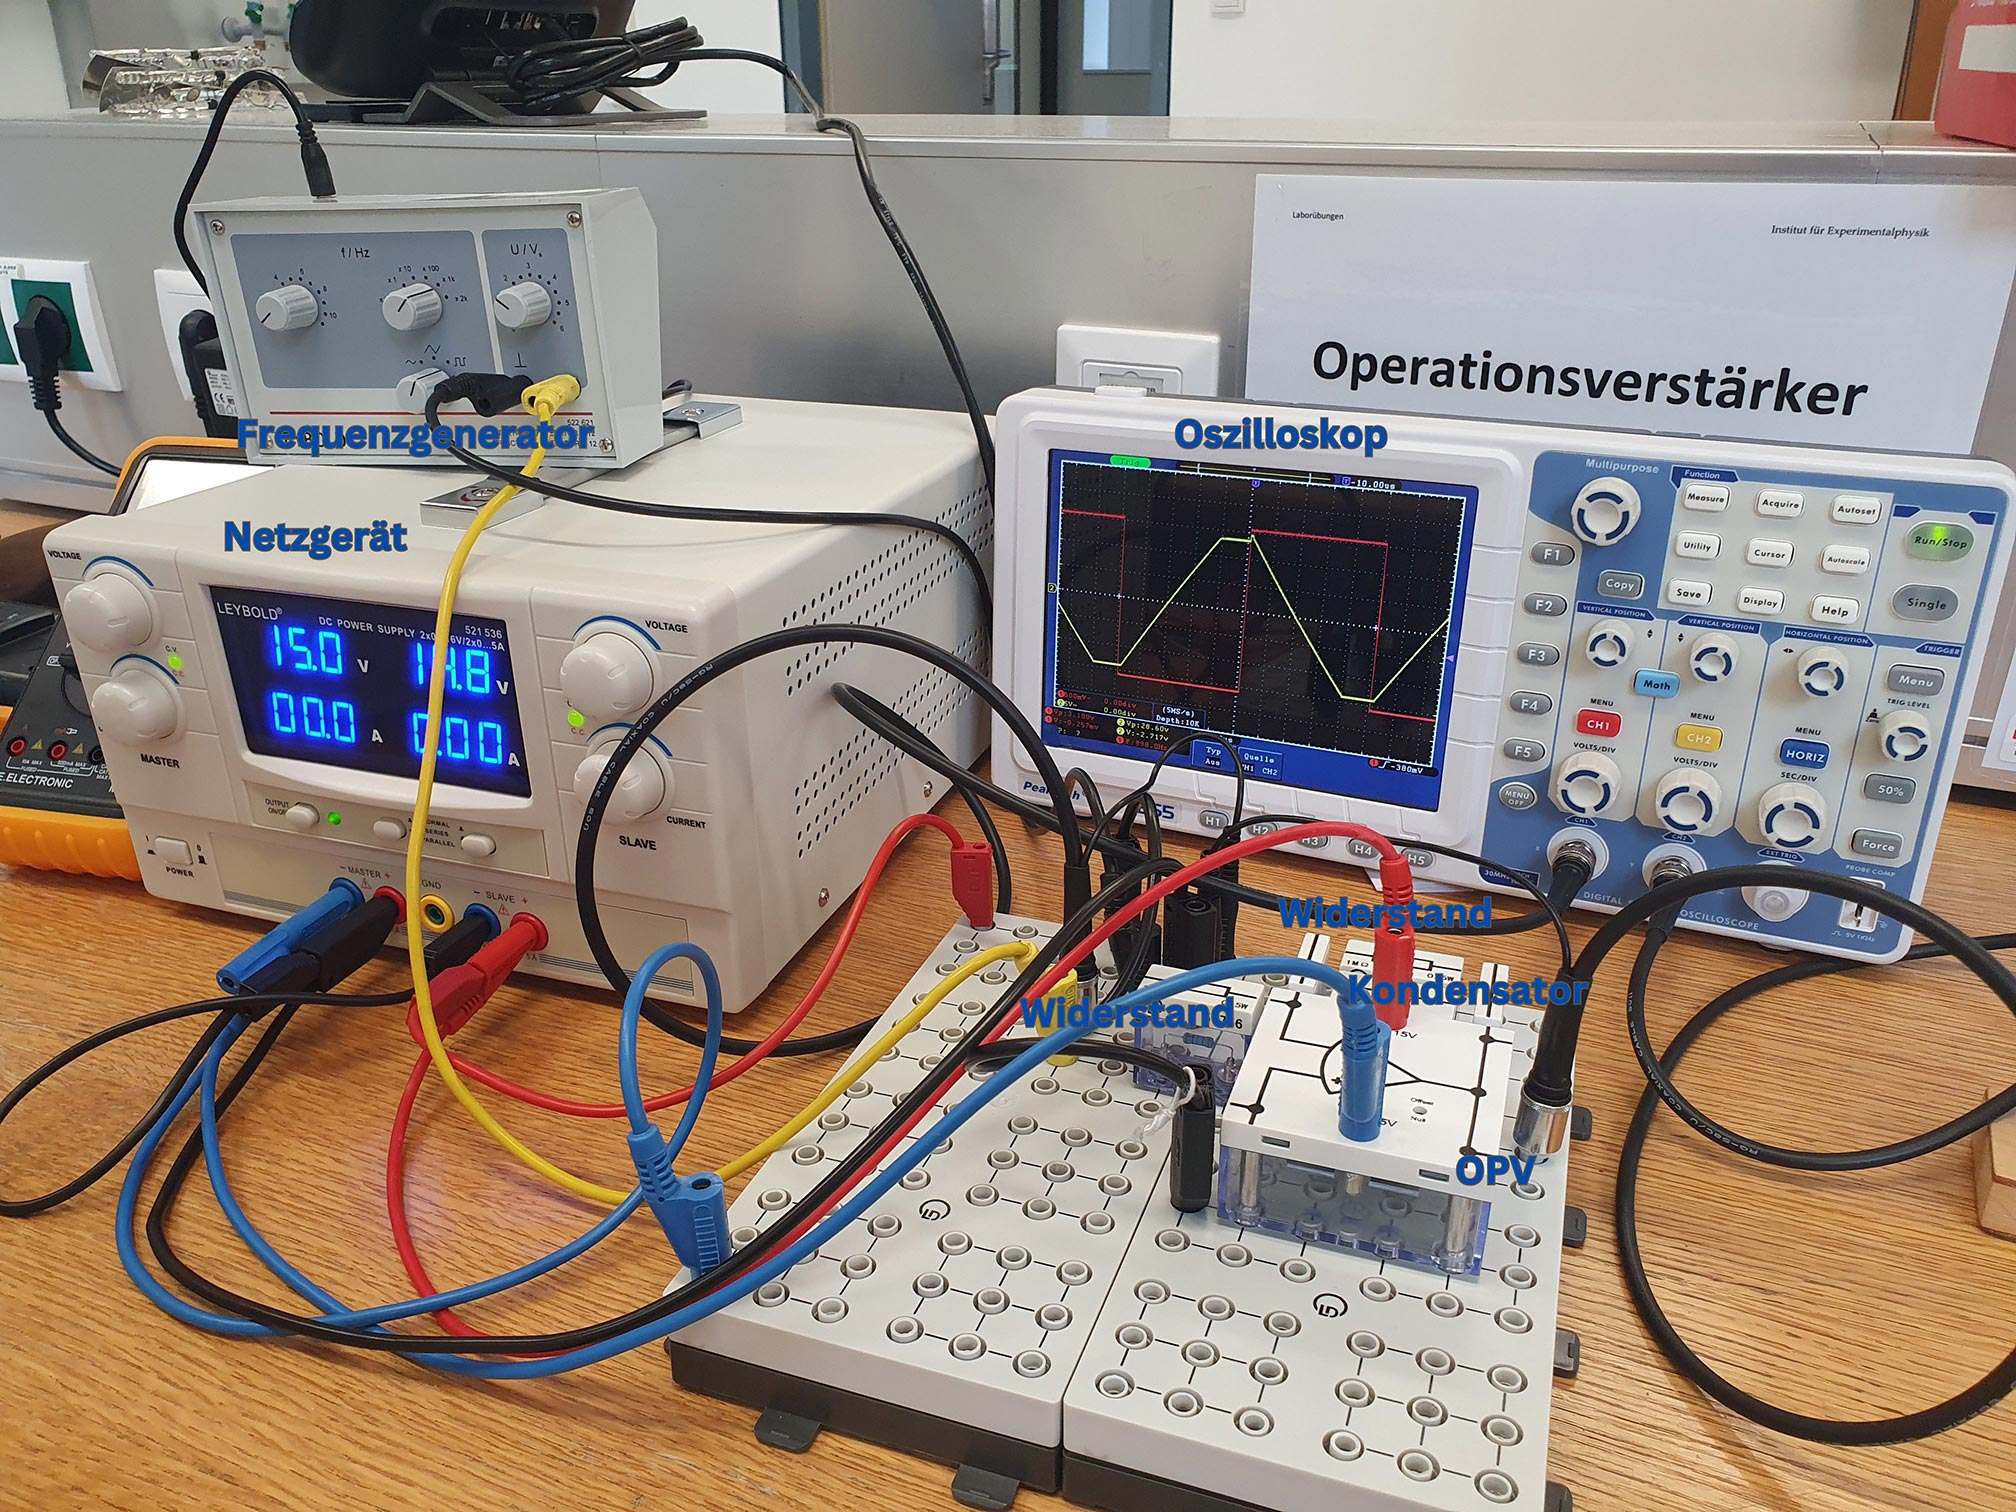
\includegraphics[width=0.4\linewidth]{nudes/messergebnisse/IntegriererIRL.jpg}
    \caption{Integrierer Schaltung und realer Aufbau \cite{teachcenter2}}
    \label{fig:SchaltungIntegrierer}
\end{figure}



\section{Geräteliste} %jo holt a listn ------------------------------

    \begin{table}[H]
        \centering
        \caption{Im Versuch verwendete Geräte und Utensilien.}
        \label{tab:geraete}
        \resizebox{\columnwidth}{!}{\begin{tabular}{|l|l|l|}
            \hline
            Gerät   & Gerätenummer  & Unsicherheit \\
            \hline
            Oszilloskop                                                                          & {n.a} & $\pm$3\% horizontal \cite{Oszi}\\
            Steckboard                                                                           & {n.a} & {n.a} \\
            Widerstände (0$\Omega$, 0.1 k$\Omega$, 0.47 k$\Omega$, 1 k$\Omega$, 1.5 k$\Omega$, 
            2.2 k$\Omega$, 4.7 k$\Omega$, 10 k$\Omega$, 15 k$\Omega$, 1 M$\Omega$)               & {n.a} & $\pm$1\% \\
            Funktionsgenerator                                                                   & {n.a} & {n.a} \\
            Netzgerät                                                                            & {n.a} & {n.a} \\
            Operationsverstärker                                                                 & {n.a} & {n.a} \\
            2x Potentiometer (100 k$\Omega$)                                                     & {n.a} & $\pm$10\% \\
            3x Digitalmultimeter                                                                 & {n.a} & $\pm$0.8\% + 3 digit \cite{DMM}\\
            Kondensatoren (10 nF, 2.2 nF, 1 $\mu F$)                                             & {n.a} & $\pm$10\% \\
            Verbindungskabel                                                                     & {n.a} & {n.a} \\
            \hline
        \end{tabular}}
    \end{table}


\section{Versuchsdurchführung \& Messergebnisse} %nachvollziehbar und klar dargestellt ------------------------------

In diesem Kapitel wird die Versuchsdurchführung dokumentiert. An den resultierenden Oszilloskopbildern stellt die rote Funktion das Eingangssignal und die gelbe Funktion das Ausgangssignal dar.

\subsection{Komperatorschaltungen}

Eingeleitet wurde der Versuch mit dem Aufbau zweier Komperatorschaltungen, welche in Abbildungen \ref{fig:GrundschaltungenAufbauIRL} zu erkennen sind. Hier soll die Funktion des OPVs als Differenzverstärker praktisch gezeigt werden.
Als Widerstände kamen zwei 47 k$\Omega$ Bauteile zum Einsatz. Das Eingangssignal der ersten Schaltung kommt von zwei mittig eingestellten 100 k$\Omega$ Potentiometern mit angelegter Netzspannung von $\pm 15 $ V, an welchen mit je einem Digitalmultimeter die Eingangsspannung festgehalten wird. Die Ausgangsspannung wird dann am OPV-Ausgang für fünf verschiedenen Potentiometerpositionen mit einem weiteren Digitalmultimeter gemessen. Die ermittelten Werte sind aus folgender Tabelle zu entnehmen.

\begin{table}[H]
    \centering
    \caption{Grundschaltung1 Messungen}
    \label{tab:Grundschaltung1Messungen}
    \begin{tabular}{| l | l | l | l |}
        \hline
        Nr. & $U_{Ein1}$ / V & $U_{Ein2}$ $\pm$ 0.01 / V & $U_{Aus1}$ $\pm$ 0.16 / V \\
        \hline
        1 & -0.0461 $\pm$ 0.0007 & -0.79 & -13.15 \\
        2 & -0.0833 $\pm$ 0.0010 & -0.79 & -13.15 \\
        3 & -0.0612 $\pm$ 0.0008 & -0.79 & -13.15 \\
        4 & -0.1069 $\pm$ 0.0013 & -0.79 & -13.15 \\
        5 & -0.0890 $\pm$ 0.0011 & -0.79 & -13.15 \\
        \hline
    \end{tabular}
\end{table}

\noindent
Bei der zweiten Komperatorschaltung wurde ein Potentiometer entfernt und durch ein Eingangssignal mit den Werten für $U{2S}$ = 3 V Sinus mit einer Frequenz von 1 kHz vom Funktionsgenerator ersetzt. Außerdem wird das resultierende Signal nun mittels Oszilloskop bildlich dargestellt:

\begin{figure}[H]
    \centering
    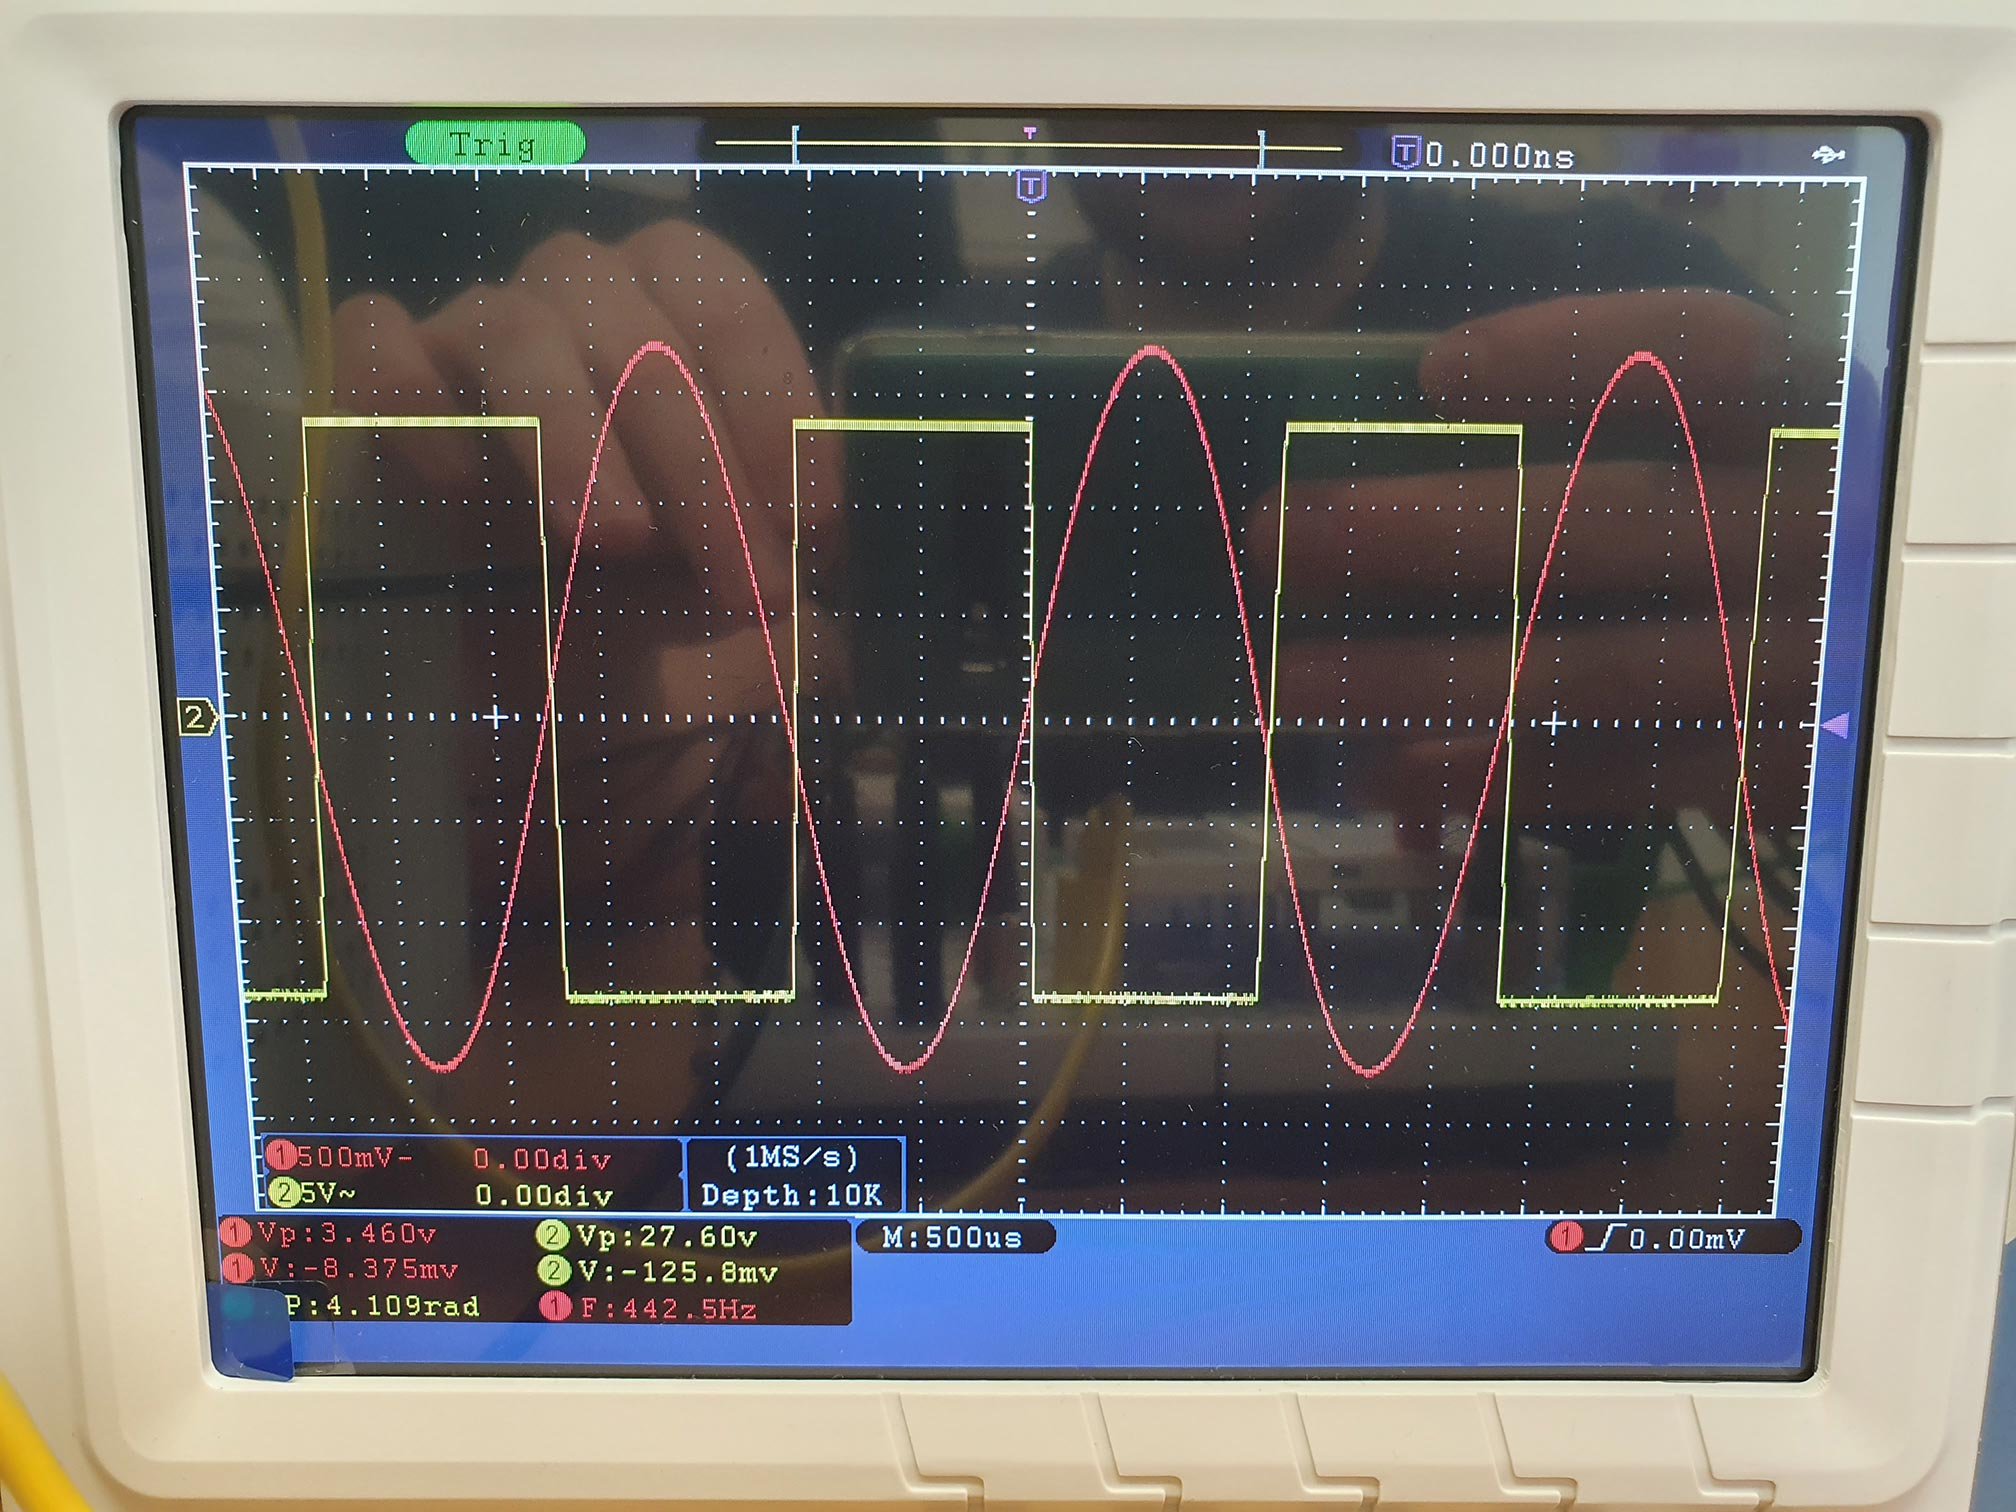
\includegraphics[width=0.4\linewidth]{nudes/messergebnisse/Grundschaltung2OsziErgebnis.jpg}
    \caption{Oszilloskopbild der zweiten Komperatorschaltung}
    \label{fig:Grundschaltung2Ergebniss}
\end{figure}

\noindent
Durch drehen am Potentiometer wird der Widerstand erhöht bzw. verringert, was zu einer Änderung am Ausgangssignal führt, auf welche im Kapitel Diskussion noch näher eingegangen wird:

\begin{figure}[H]
    \centering
    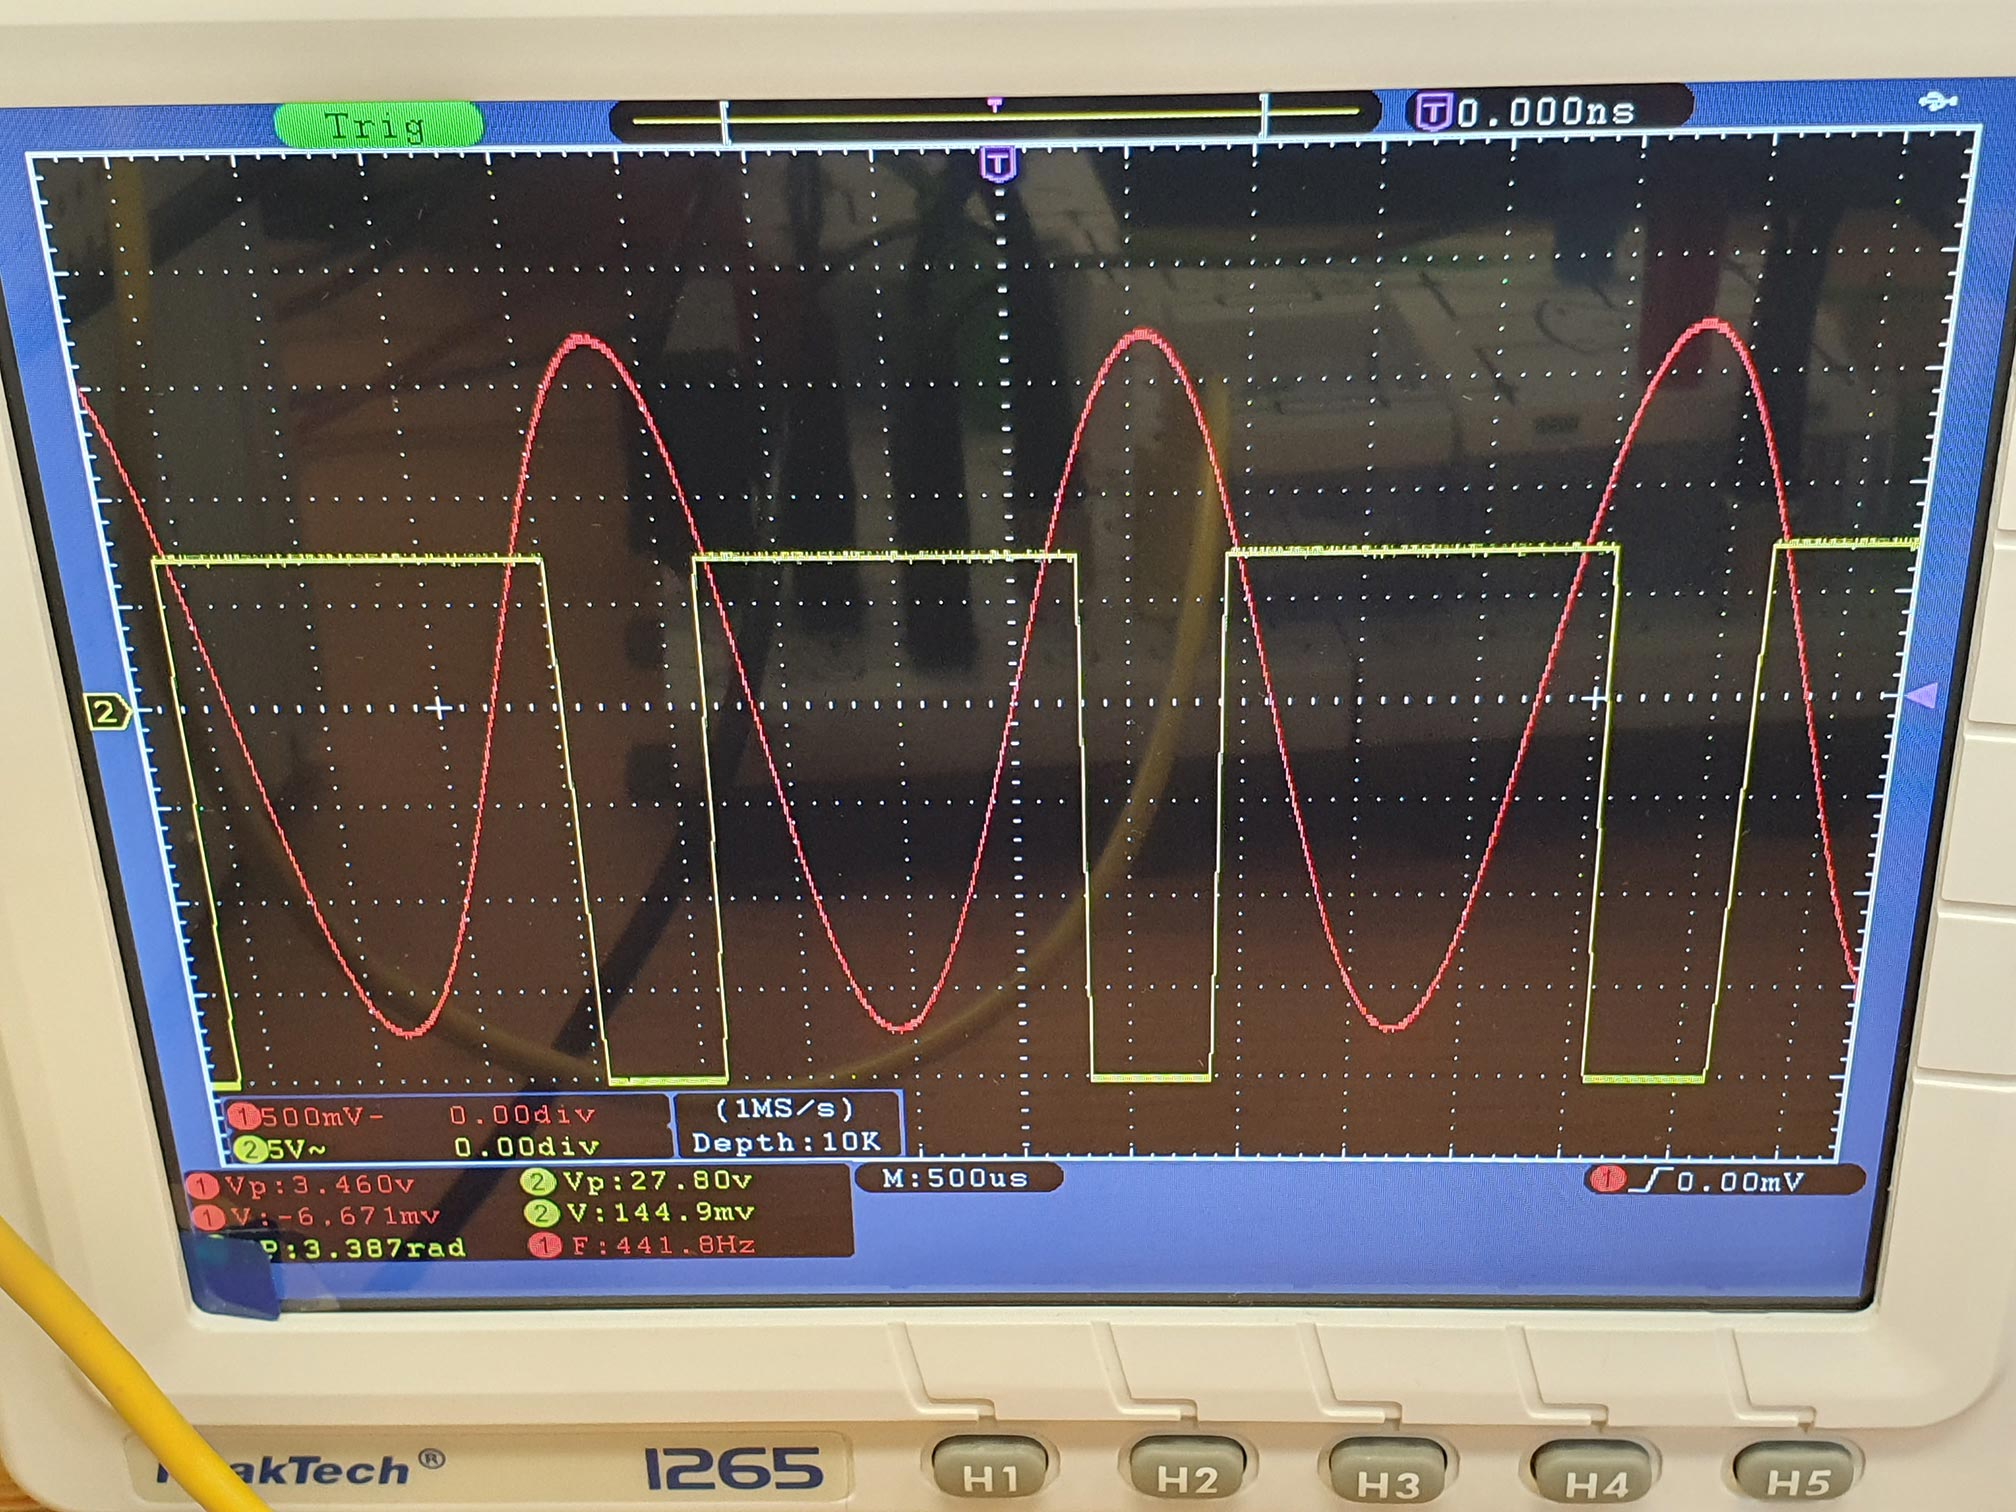
\includegraphics[width=0.4\linewidth]{nudes/messergebnisse/Grundschaltung2OsziErgebnislinks.jpg}
    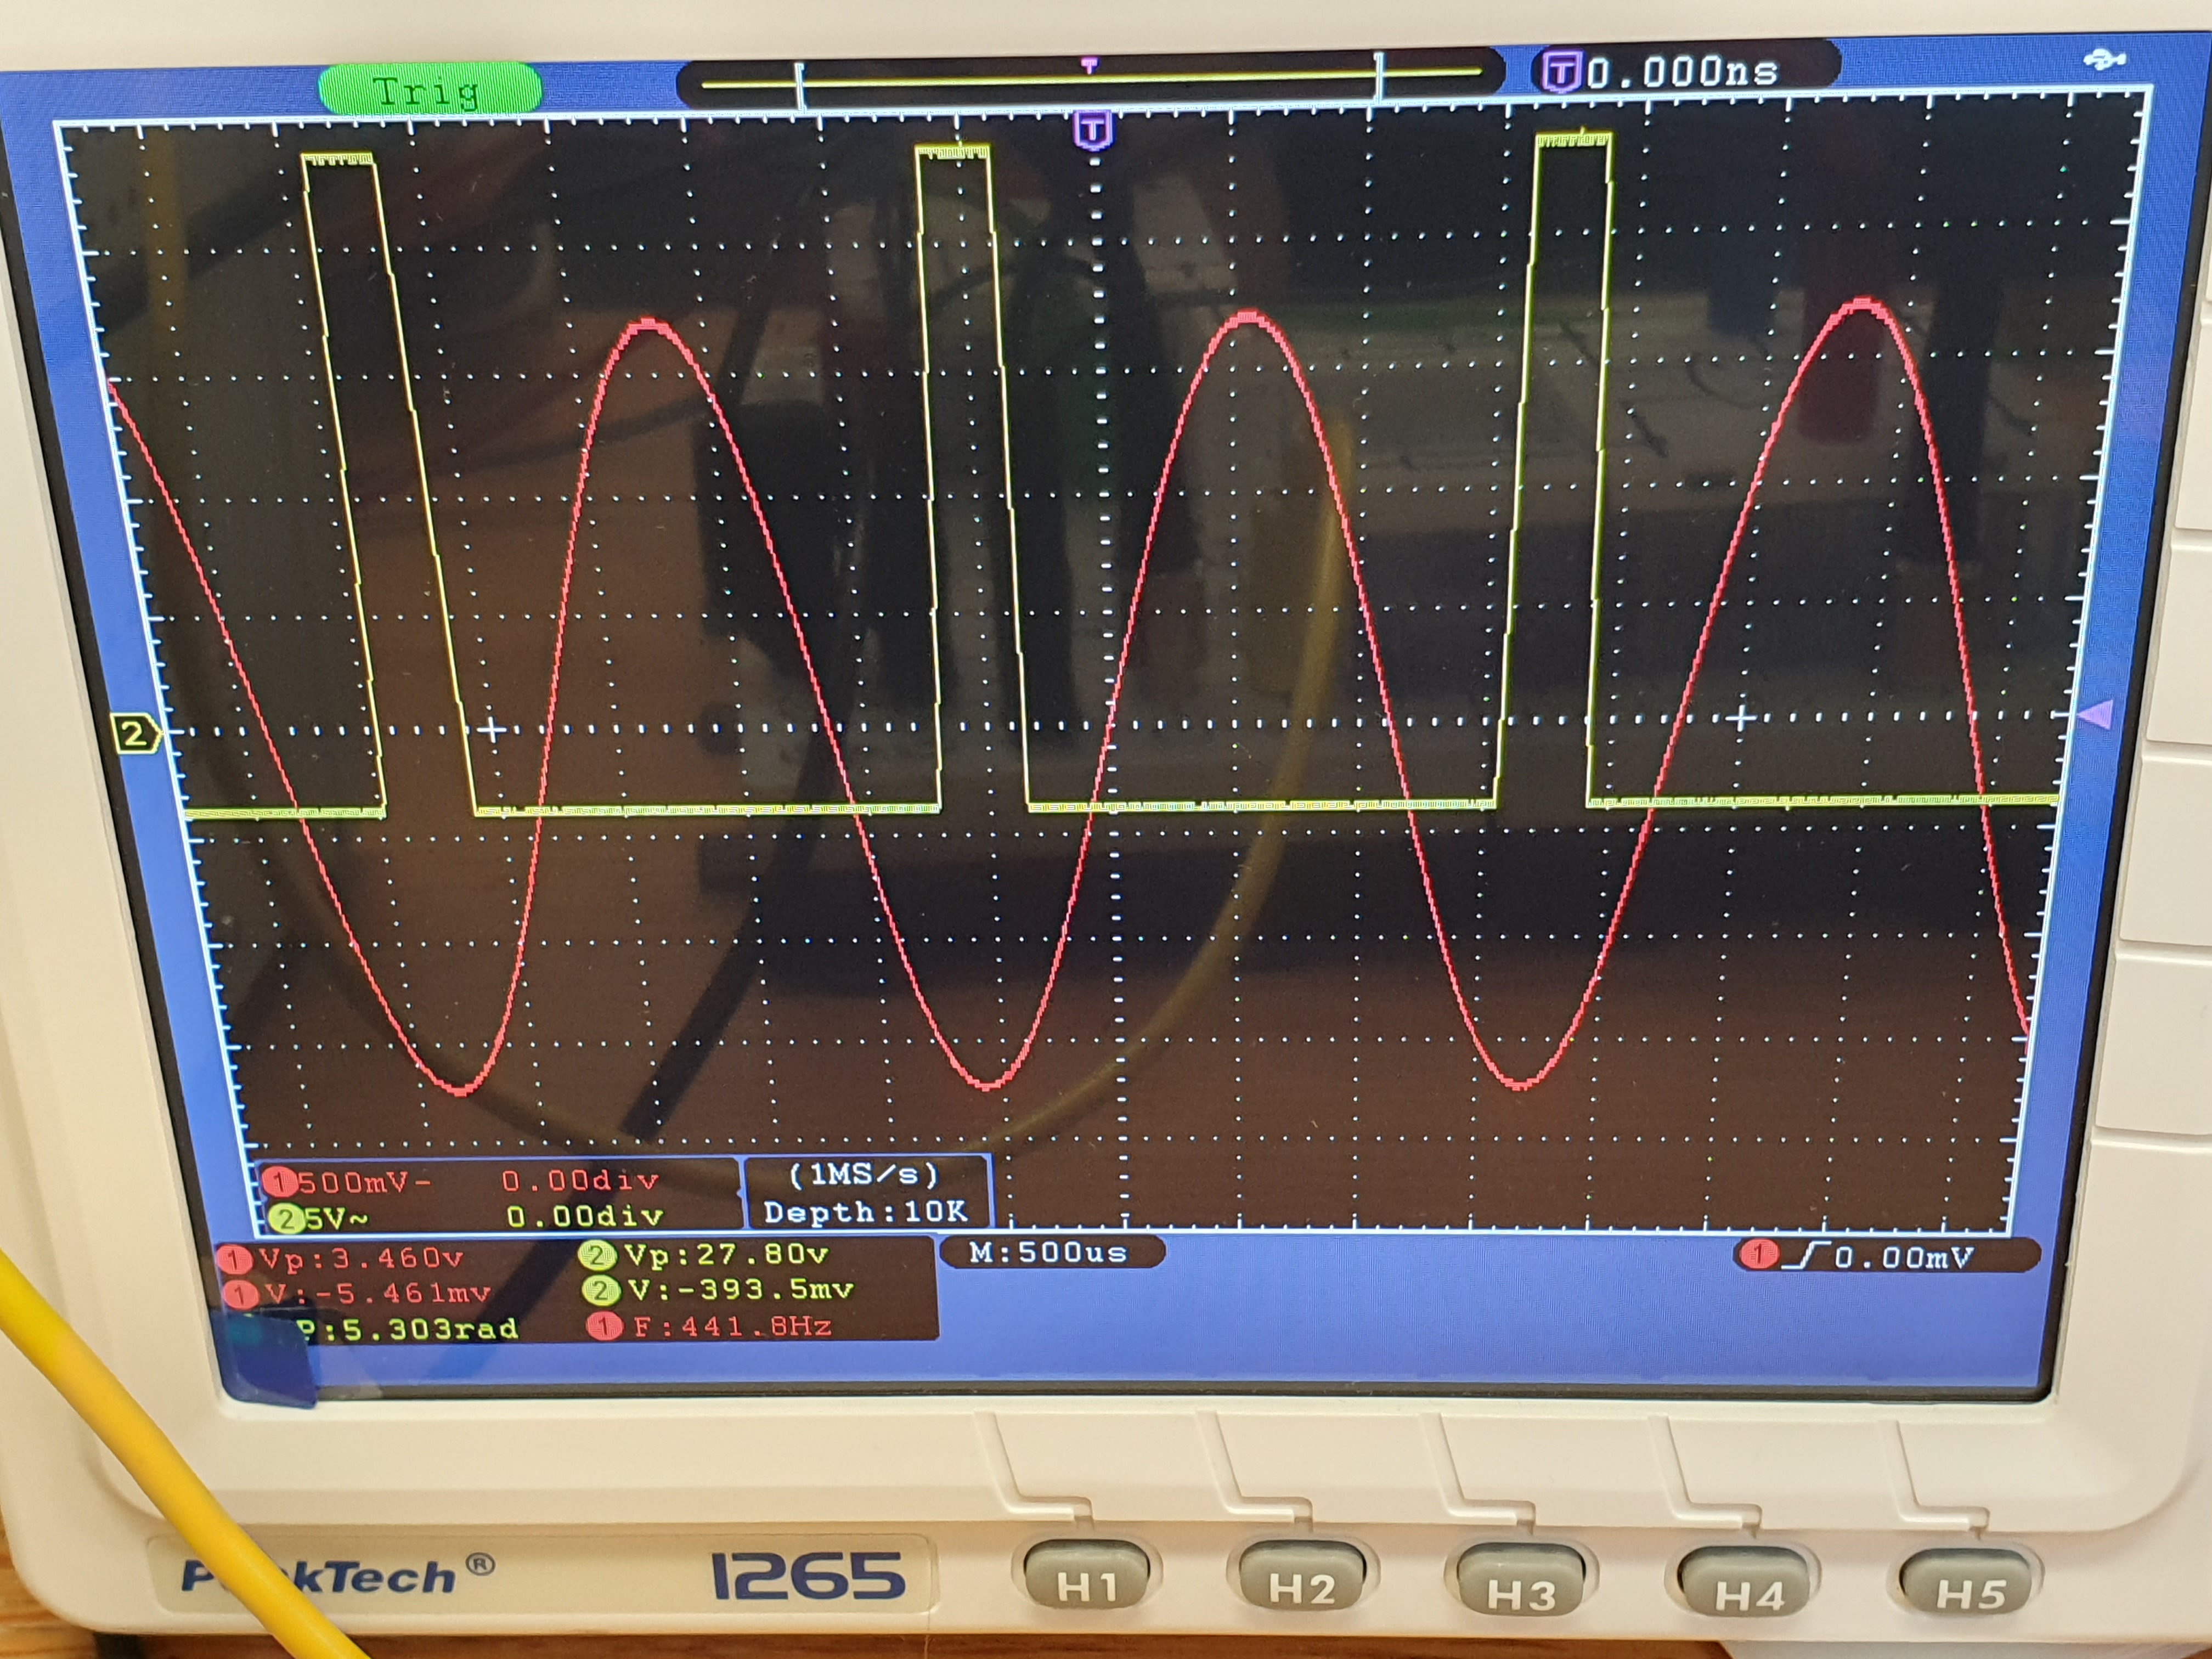
\includegraphics[width=0.4\linewidth]{nudes/messergebnisse/Grundschaltung2OsziErgebnisrechts.jpg}
    \caption{Oszilloskopbild der zweiten Komperatorschaltung mit größer/kleiner gestellten Widerstand}
    \label{fig:Grundschaltung2ErgebnissPoti}
\end{figure}

\subsection{Invertierender Verstärker}

Nachdem die Funktion eines OPVs nun nicht nur grundlegend bekannt war, sondern nun auch anhand eines Experimentes nachgewiesen wurde, konnten die ersten größeren Schaltungen realisiert werden. \newline

\noindent
Als erstes wurde dabei ein invertierender Verstärker laut Abbildungen \ref{fig:SchaltungInvertierenderVerstärker} in die Tat umgesetzt. Auch hier wurde wieder auf zwei 47 k$\Omega$ Widerstände mit einer eingehenden Netzspannung von $\pm$ 15 V vom Netzgerät gesetzt.
Dabei wurden drei verschiedene Widerstände $R_{2}$ mit einmal 10 k$\Omega$, einmal 33 10 k$\Omega$ und einmal 100 k$\Omega$ verwendet. Zu jedem Widerstand wurde die Eingangsspannung jeweils mit dem Potentiometer so verändert, dasss ungefähr 1.5 V, 1.0 V, 0.5 V, 0 V, -0.5 V, -1.0 V und -1.5 V in den OPV fließen. 
Somit konnten zu jedem der drei verwendeten Widerstände $R_{2}$ jeweils sieben Werte in folgenden Tabellen festgehalten werden:

\begin{table}[H]
    \centering
    \caption{Invertierender OPV 10 k$\Omega$ $U_{Aus}$ Messung}
    \label{tab:IoVerstärkungenGemessen10}
    \begin{tabular}{| l | l | l | l |}
        \hline
        Nr. & Zieleingangsspannungen / V & $U_{Ein}$ / V & $U_{Aus}$ / V \\
        \hline
        1 &  1.5 &  1.511 $\pm$ 0.016 & -1.530 $\pm$ 0.016 \\
        2 &  1.0 &  1.022 $\pm$ 0.012 & -1.035 $\pm$ 0.012 \\
        3 &  0.5 &  0.499 $\pm$ 0.007 & -0.505 $\pm$ 0.008 \\
        4 &  0.0 &  0.024 $\pm$ 0.005 & -0.024 $\pm$ 0.005 \\
        5 & -0.5 & -0.521 $\pm$ 0.008 &  0.521 $\pm$ 0.008 \\
        6 & -1.0 & -1.039 $\pm$ 0.012 &  1.039 $\pm$ 0.012 \\
        7 & -1.5 & -1.532 $\pm$ 0.016 &  1.532 $\pm$ 0.016 \\
        \hline
    \end{tabular}
\end{table}

\begin{table}[H]
    \centering
    \caption{Invertierender OPV 33 k$\Omega$ $U_{Aus}$ Messung}
    \label{tab:IoVerstärkungenGemessen33}
    \begin{tabular}{| l | l | l | l |}
        \hline
        Nr. & Zieleingangsspannungen / V & $U_{Ein}$ / V & $U_{Aus}$ / V \\
        \hline
        1 &  1.5 &  1.486 $\pm$ 0.015 & -4.95  $\pm$  0.07 \\
        2 &  1.0 &  1.011 $\pm$ 0.012 & -3.36  $\pm$  0.06 \\
        3 &  0.5 &  0.511 $\pm$ 0.008 & -1.706 $\pm$ 0.017 \\
        4 &  0.0 &  0.010 $\pm$ 0.004 & -0.031 $\pm$ 0.001 \\
        5 & -0.5 & -0.511 $\pm$ 0.008 &  1.699 $\pm$ 0.017 \\
        6 & -1.0 & -1.013 $\pm$ 0.012 &  3.368 $\pm$ 0.06  \\
        7 & -1.5 & -1.496 $\pm$ 0.015 &  4.980 $\pm$ 0.07  \\
        \hline
    \end{tabular}
\end{table}

\begin{table}[H]
    \centering
    \caption{Invertierender OPV 100 k$\Omega$ $U_{Aus}$ Messung}
    \label{tab:IoVerstärkungenGemessen100}
    \begin{tabular}{| l | l | l | l |}
        \hline
        Nr. & Zieleingangsspannungen / V & $U_{Ein}$ / V & $U_{Aus}$ / V \\
        \hline
        1 &  1.5 &  1.464 $\pm$ 0.015 & -13.14  $\pm$ 0.14  \\
        2 &  1.0 &  1.054 $\pm$ 0.012 & -10.70  $\pm$ 0.12  \\
        3 &  0.5 &  0.519 $\pm$ 0.008 &  -5.26  $\pm$ 0.08  \\
        4 &  0.0 & -0.009 $\pm$ 0.004 &  -0.094 $\pm$ 0.001 \\
        5 & -0.5 & -0.493 $\pm$ 0.007 &   5.01  $\pm$ 0.08  \\
        6 & -1.0 & -1.036 $\pm$ 0.012 &  10.53  $\pm$ 0.12  \\
        7 & -1.5 & -1.656 $\pm$ 0.017 &  14.33  $\pm$ 0.15  \\
        \hline
    \end{tabular}
\end{table}


\subsection{Nichtinvertierender Verstärker}

Das Gegenstück zum invertierenden Verstärker bilder der nichtinvertierende Verstärker, welcher ebenfalls laut Abbildung \ref{fig:SchaltungNichtInvertierenderVerstärker} zusammengebaut wurde. \newline

\noindent
Zunächst wurden $R_{1}$ und $R_{2}$ gleich mit 10 k$\Omega$ gewählt. Am Funktionsgenerator wurde eine Eingangsspannung von 4 V Sinus mit einer Frequenz von 200 Hz gewählt. Das resultierende Oszilloskopbild ist in folgender Abbildung ersichtlich:

\begin{figure}[H]
    \centering
    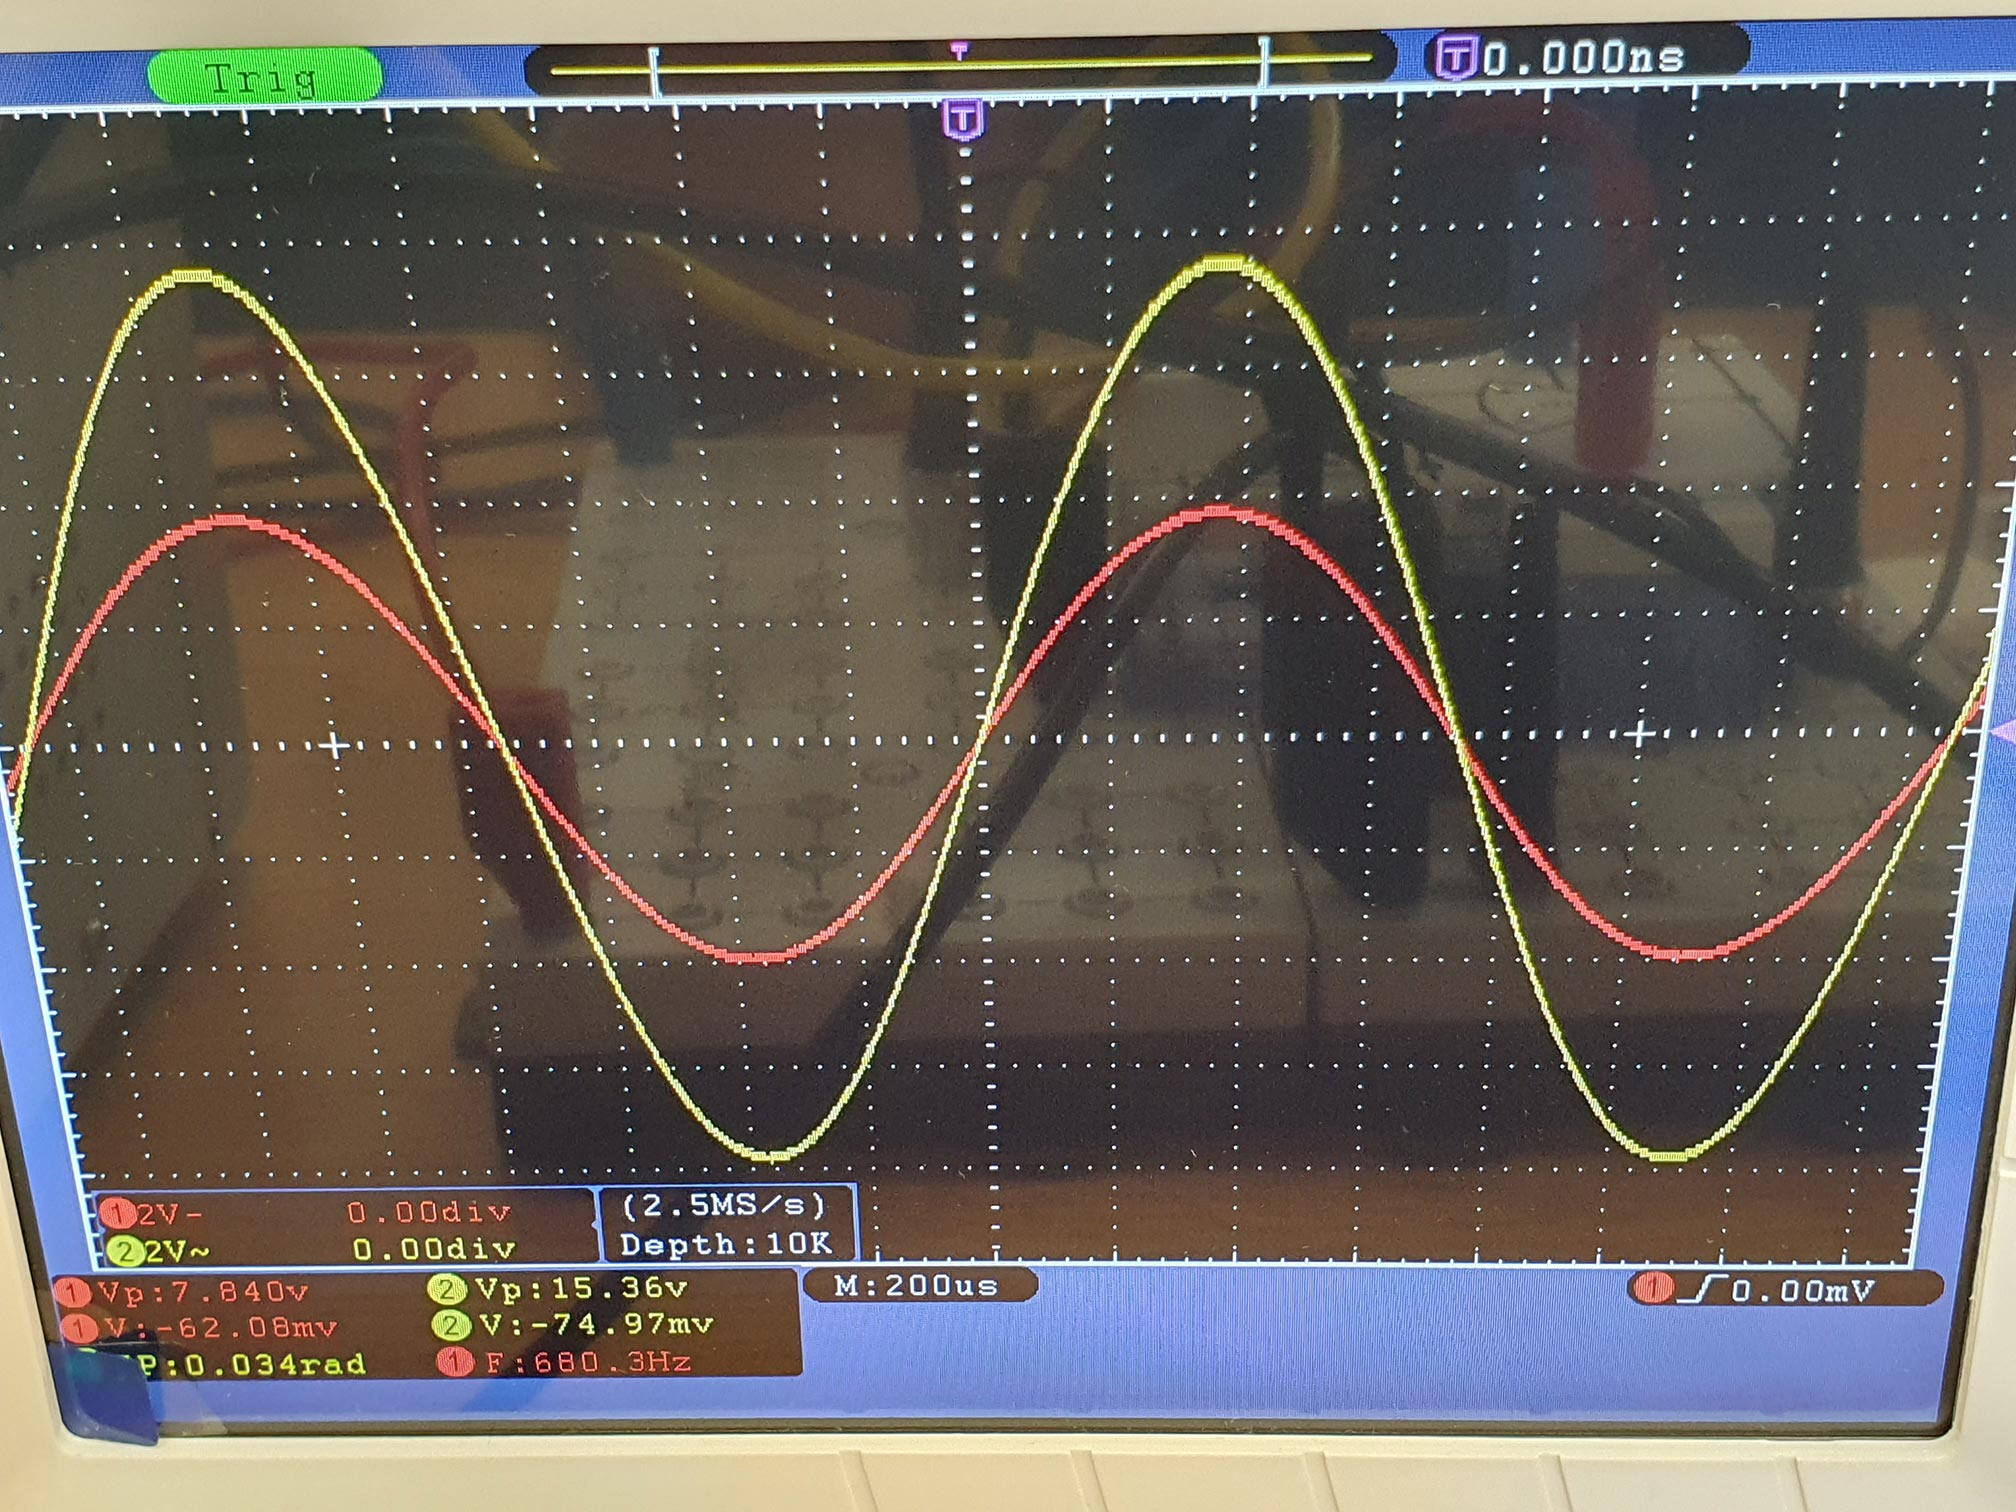
\includegraphics[width=0.4\linewidth]{nudes/messergebnisse/NichtInv10kund10kErgebniss.jpg}
    \caption{Oszilloskopbild des nichtinvertierenden OPVs mit $R_{1}$ = $R_{2}$ = 10 k$\Omega$}
    \label{fig:Nichtinvertierender10k10kOszibild}
\end{figure}

\noindent
Nun wurden die Widerstände etwas variiert. $R_{2}$ wurde zwischen 0 k$\Omega$, 0.47 k$\Omega$, 1.5 k$\Omega$, 2.2 k$\Omega$, 4.7 k$\Omega$ und 10 k$\Omega$ gewechselt, der Widerstand $R_{1}$ blieb dauerhaft bei 1 k$\Omega$. Als Eingangssignal vom Funktionsgenerator wurden 1 V Sinus mit 1 kHz eingestellt.
Die daraus resultierenden Oszilloskopbilder wurden bildlich und schriftlich in folgenden Bildern und Tabelle festgehalten. Das Oszilloskop wurde dabei immer so eingestellt, dass die beiden Amplitudenpeaks zur Bestimmung der Verhältnisse gut sichtbar sind.

\begin{figure}[H]
    \centering
    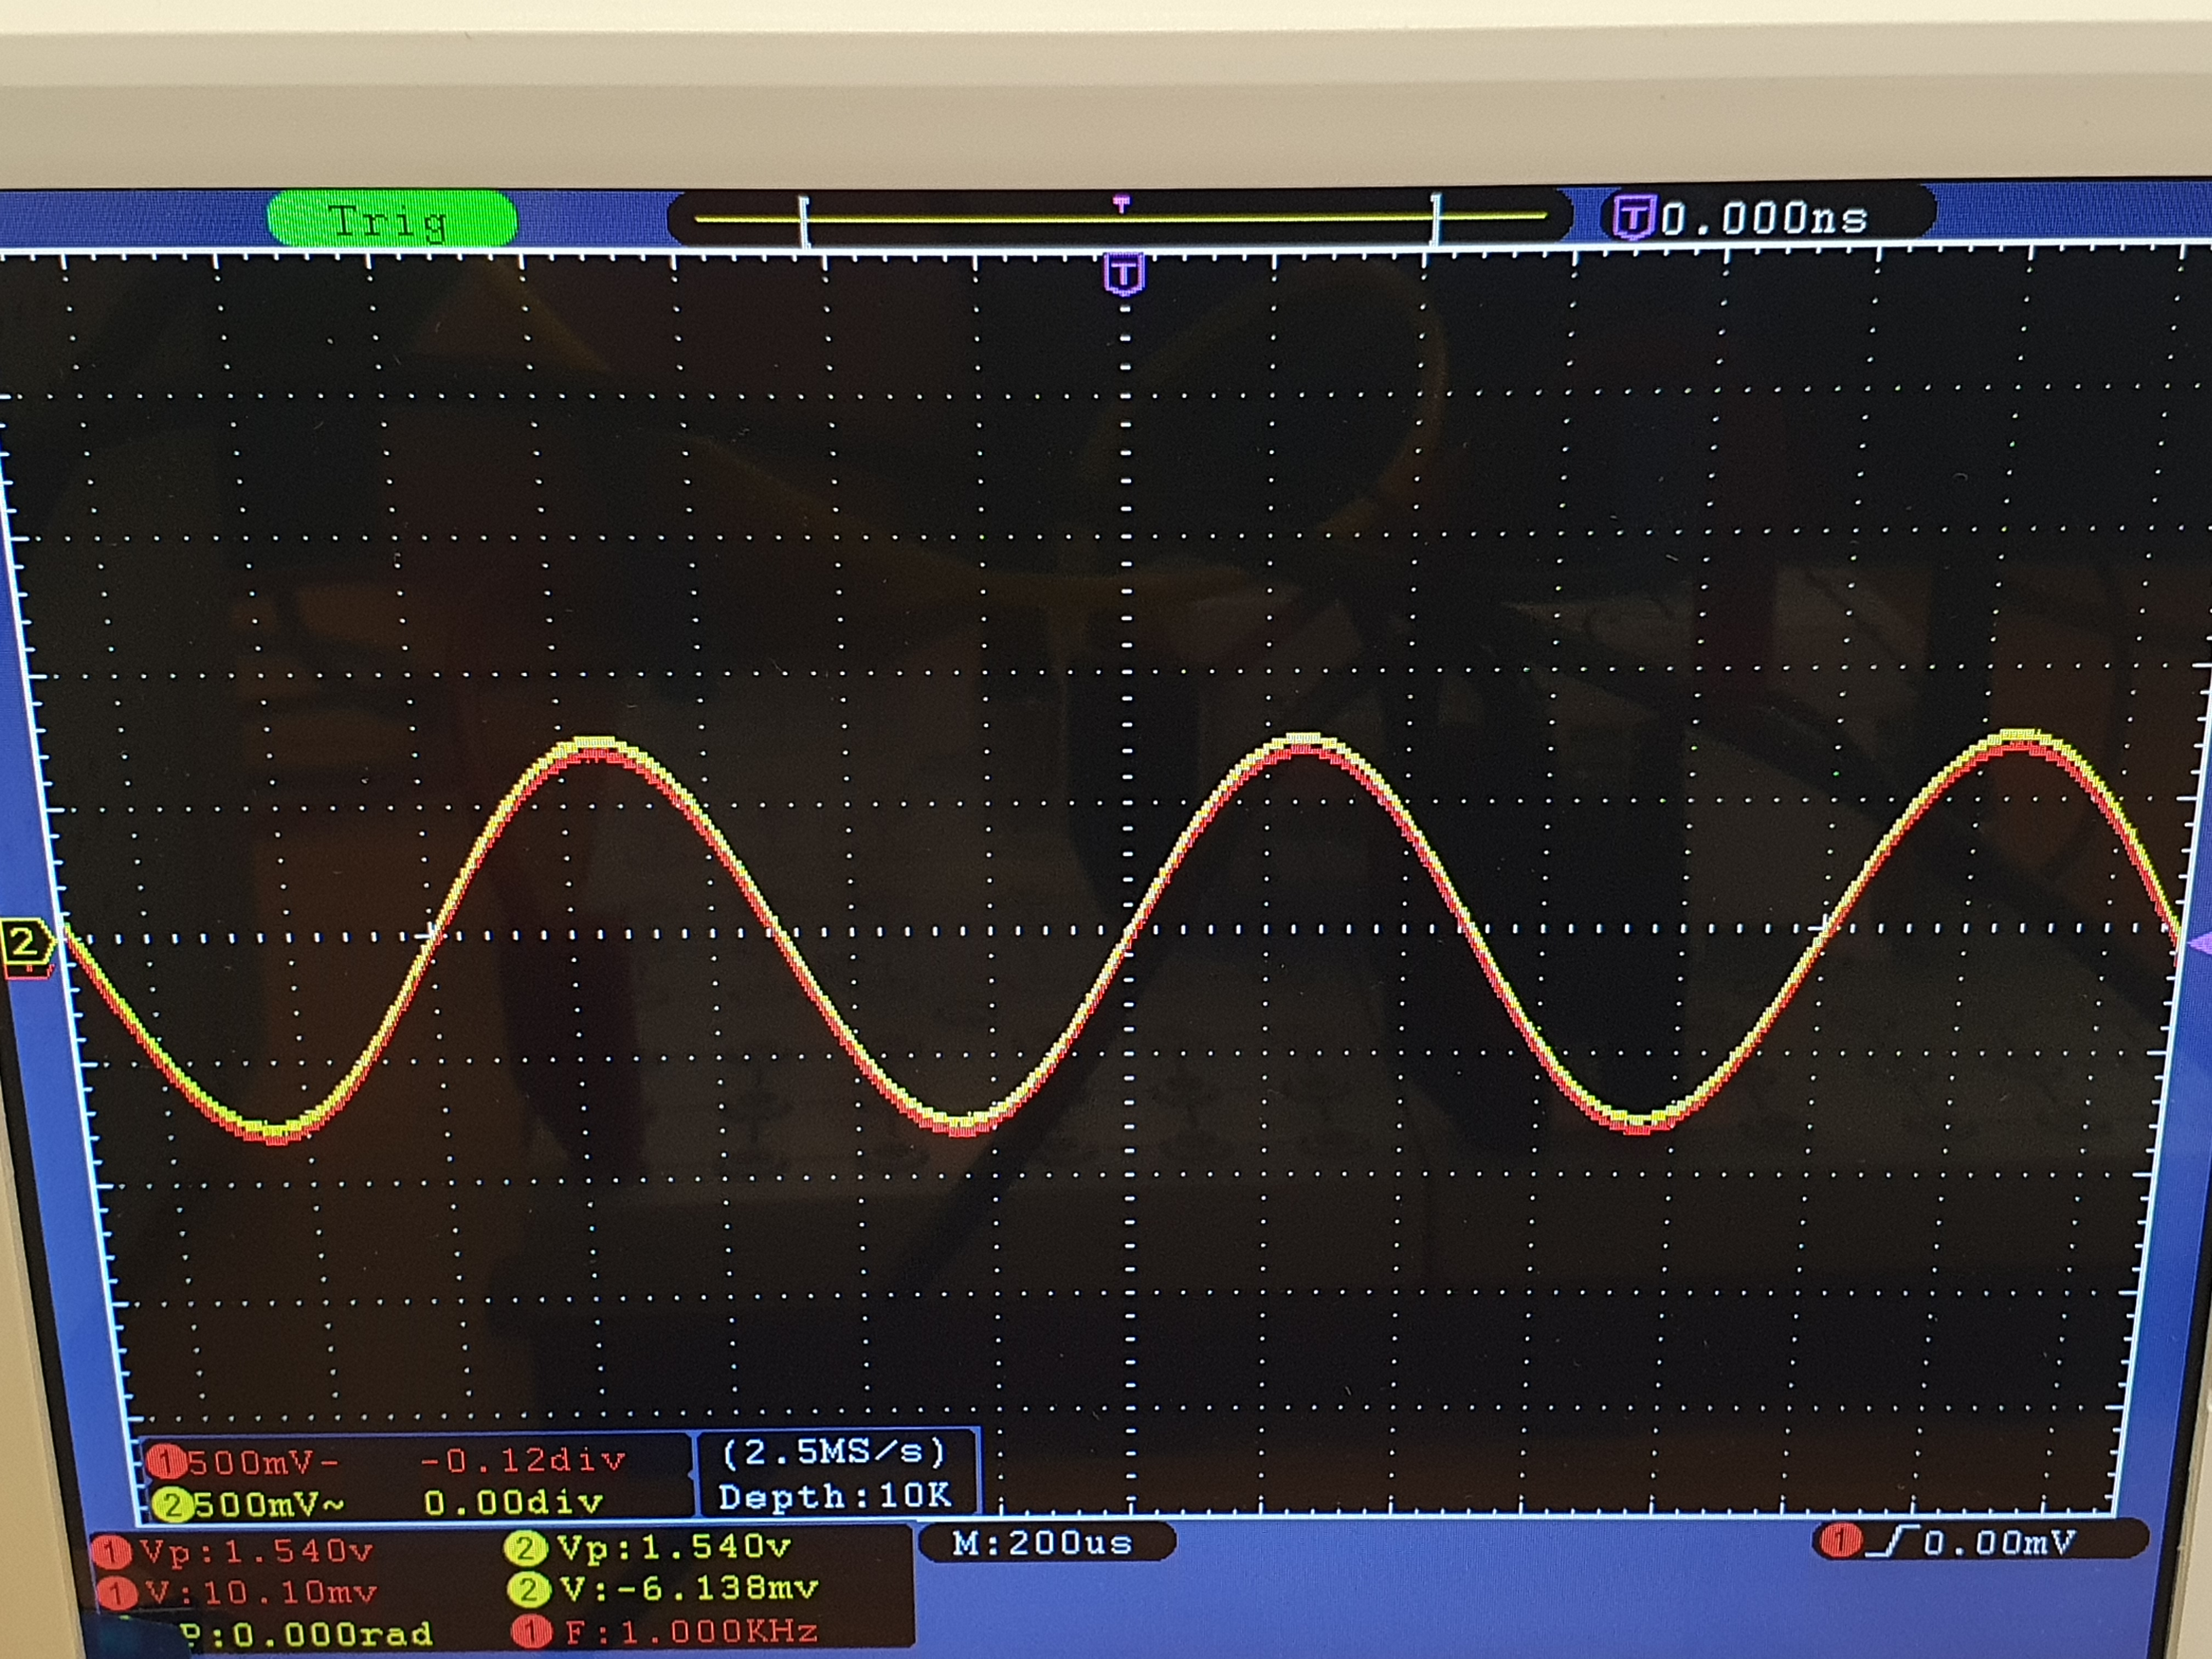
\includegraphics[width=0.4\linewidth]{nudes/messergebnisse/NichtInv1kund0kErgebnis.jpg}
    \caption{Oszilloskopbild des nichtinvertierenden OPVs mit $R_{2}$ = 0 k$\Omega$}
    \label{fig:Nichtinvertierender1k0kOszibild}
\end{figure}

\begin{figure}[H]
    \centering
    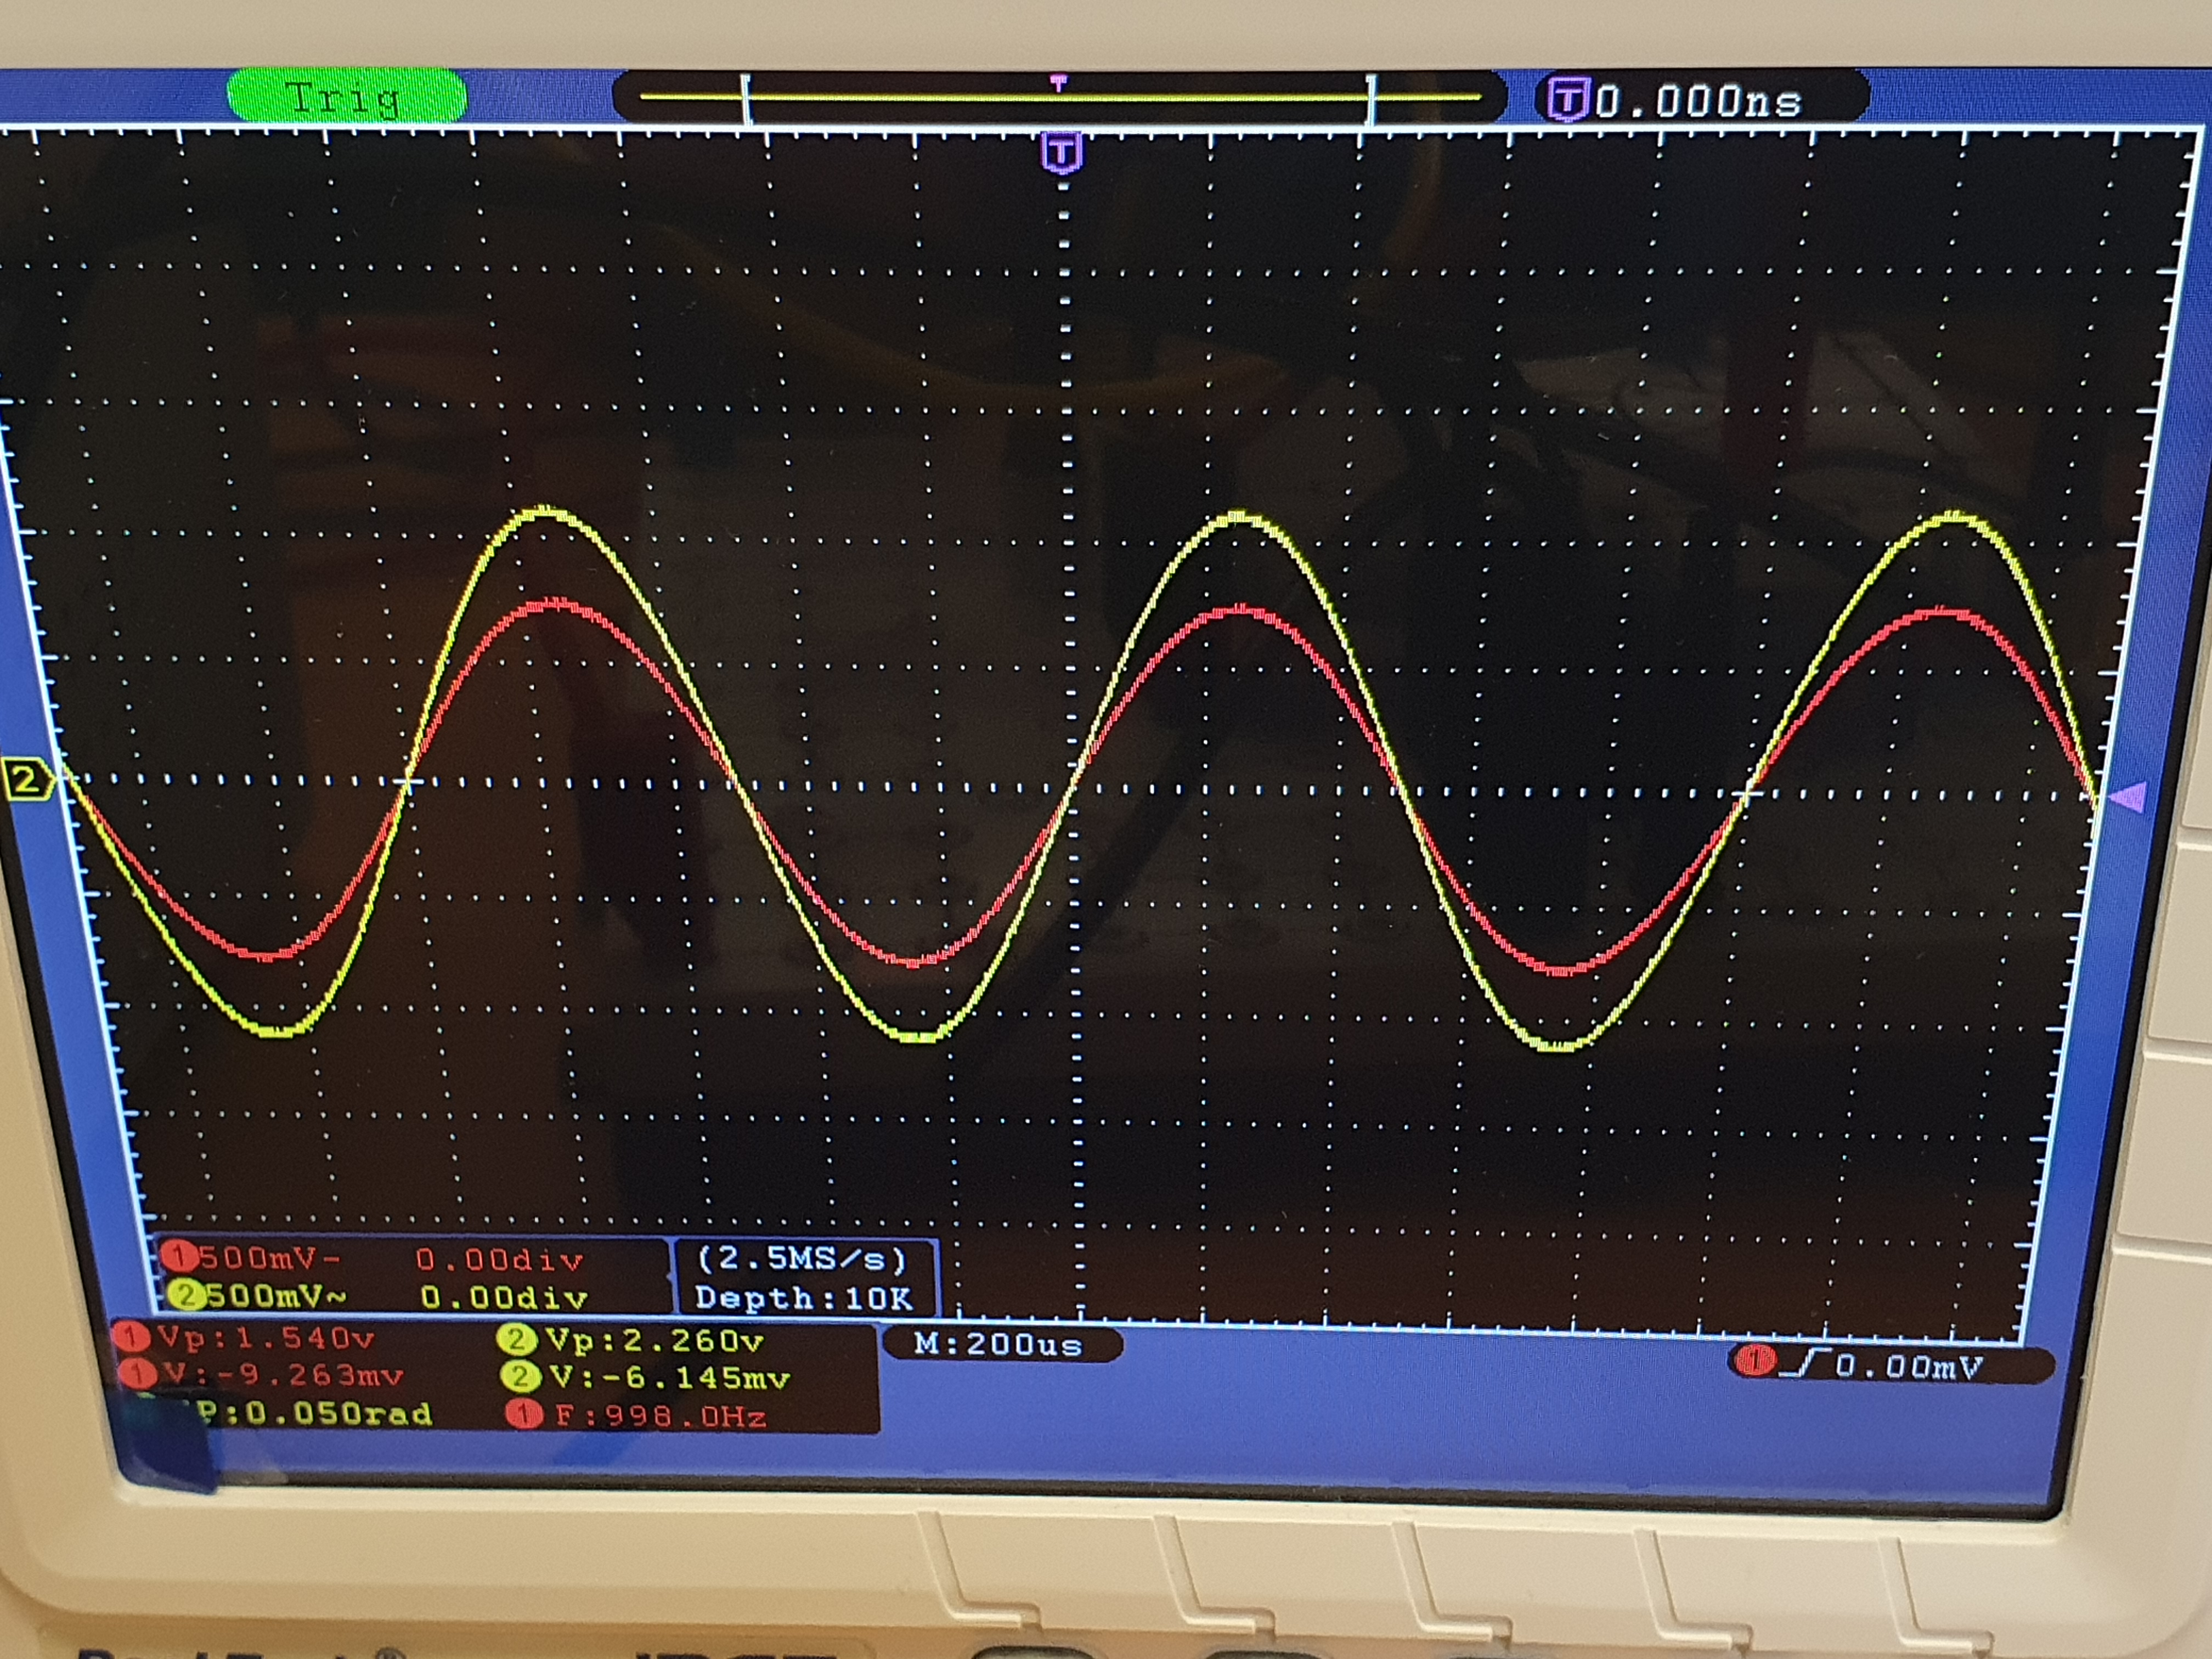
\includegraphics[width=0.4\linewidth]{nudes/messergebnisse/NichtInv1kund0.47kErgebnis.jpg}
    \caption{Oszilloskopbild des nichtinvertierenden OPVs mit $R_{2}$ = 0.47 k$\Omega$}
    \label{fig:Nichtinvertierender1k0.47kOszibild}
\end{figure}

\begin{figure}[H]
    \centering
    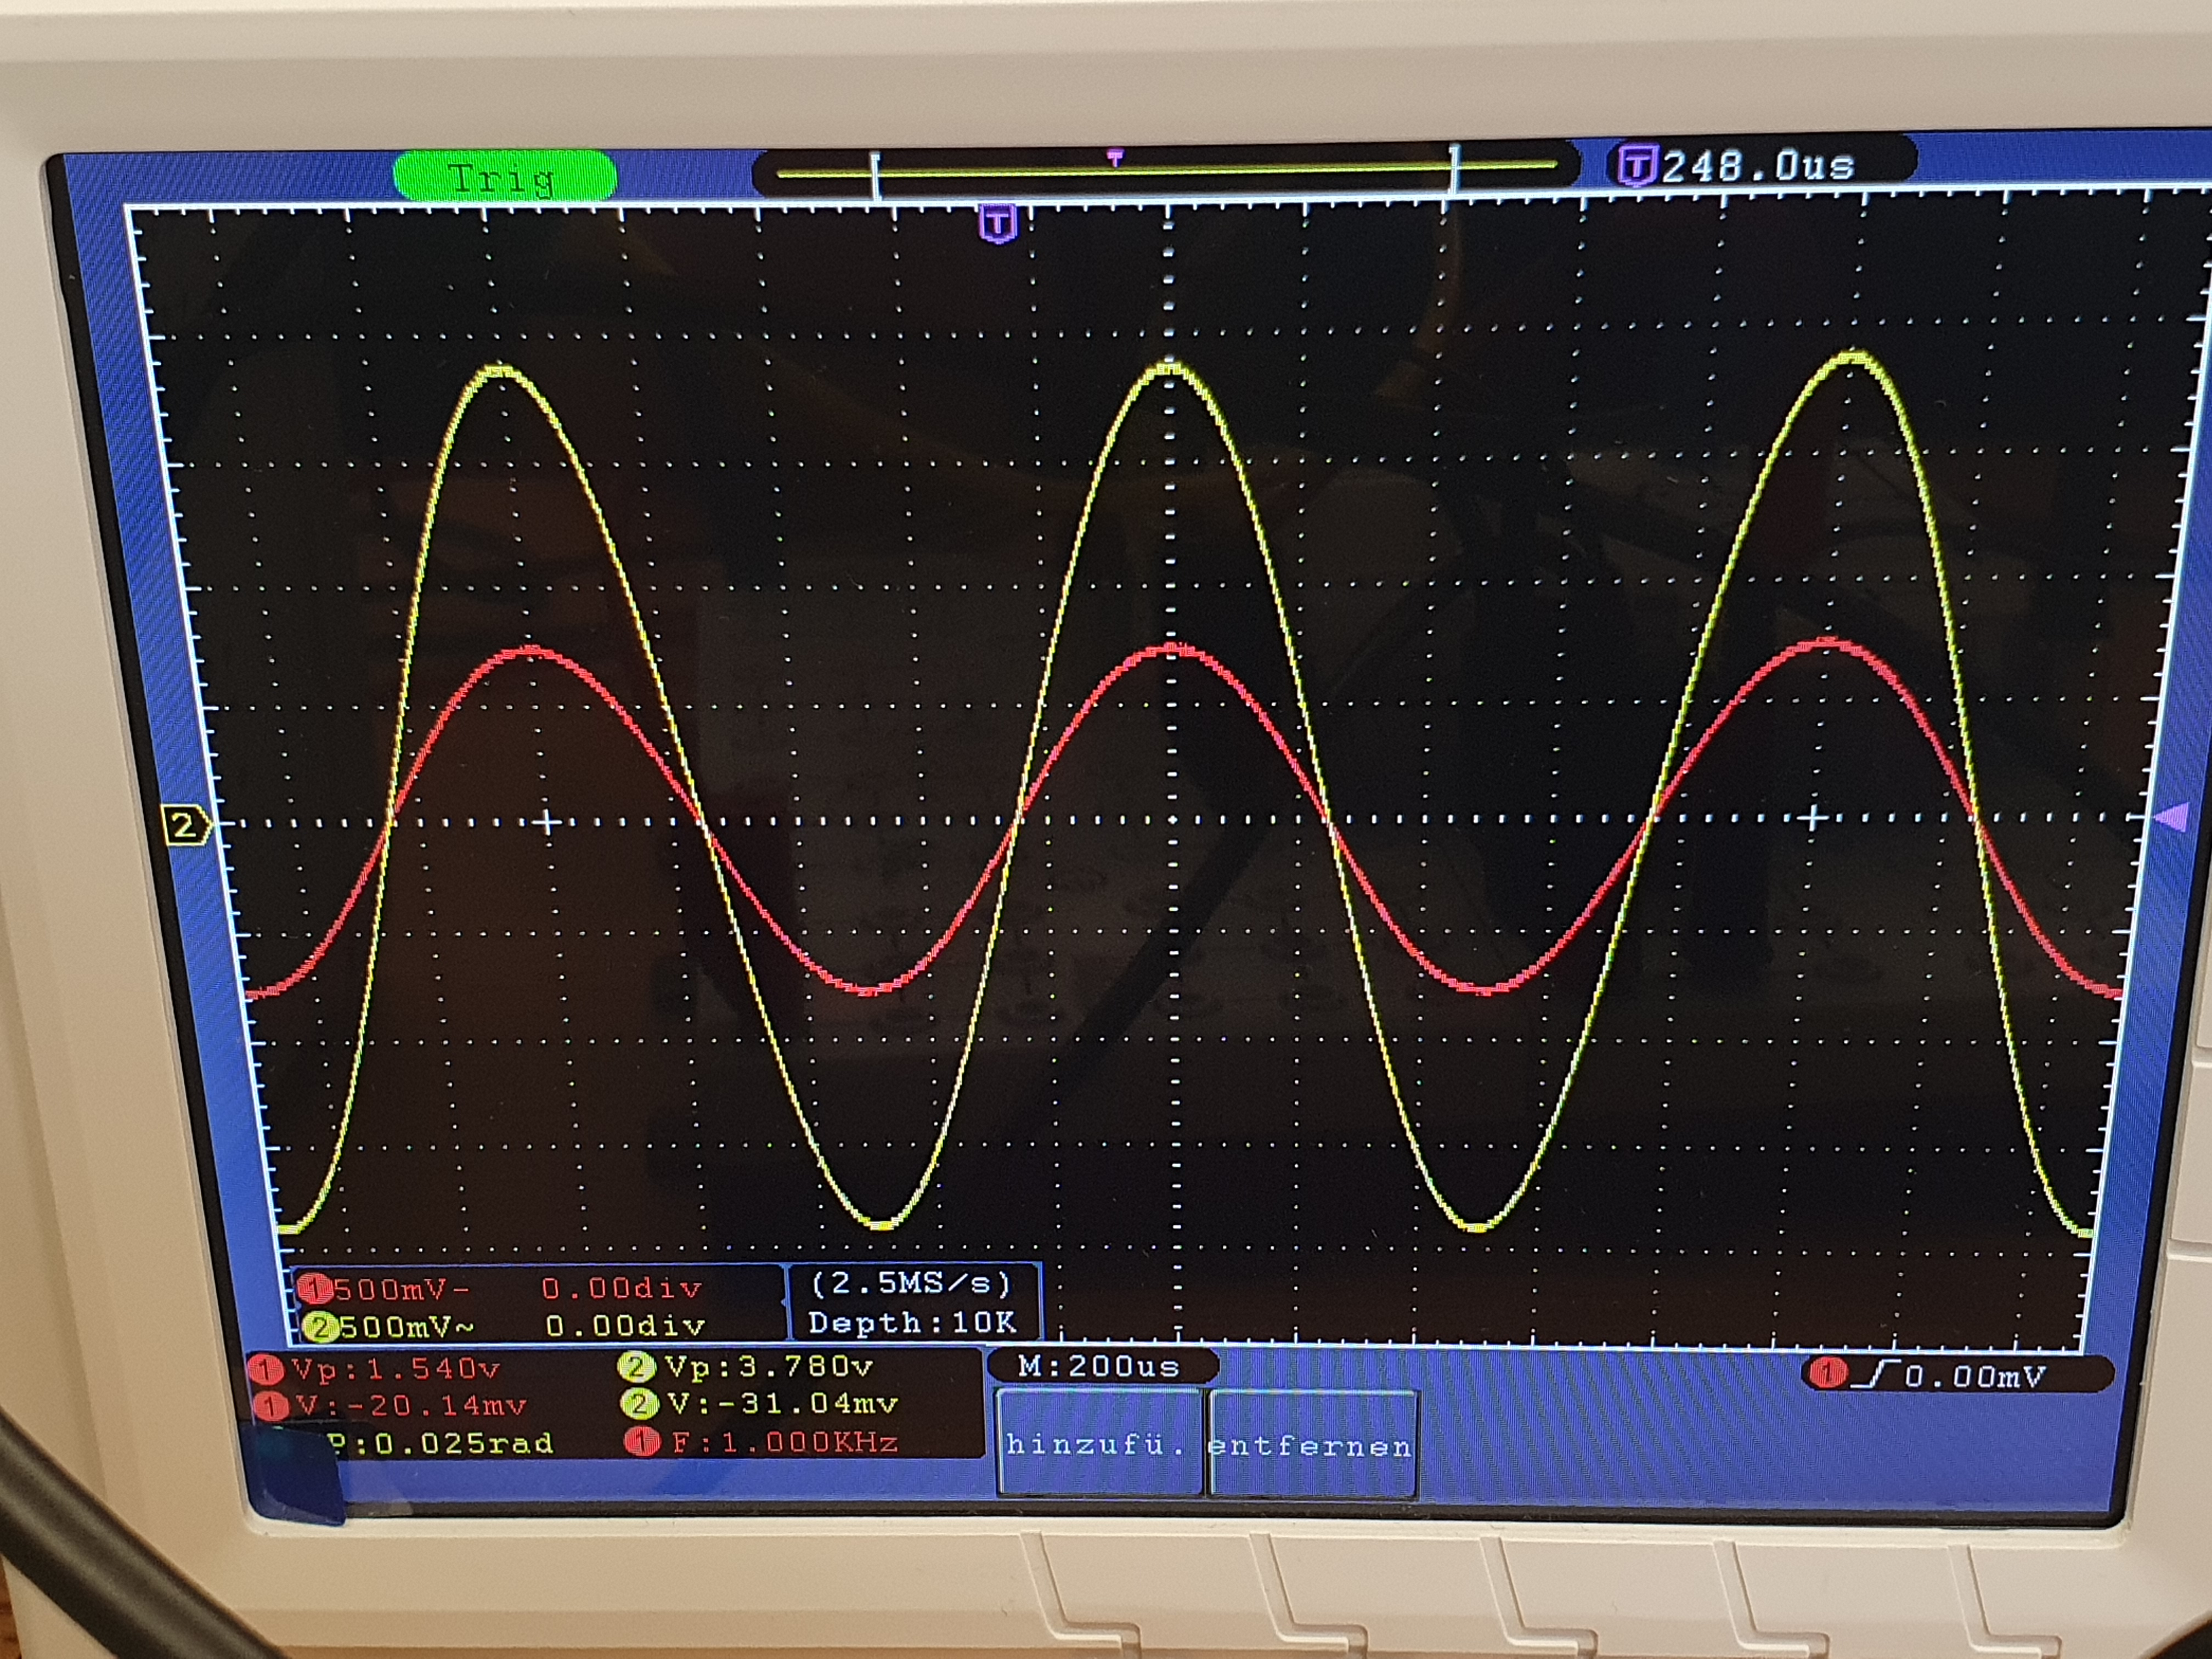
\includegraphics[width=0.4\linewidth]{nudes/messergebnisse/NichtInv1kund1.5kErgebnis.jpg}
    \caption{Oszilloskopbild des nichtinvertierenden OPVs mit $R_{2}$ = 1.5 k$\Omega$}
    \label{fig:Nichtinvertierender1k1.5kOszibild}
\end{figure}

\begin{figure}[H]
    \centering
    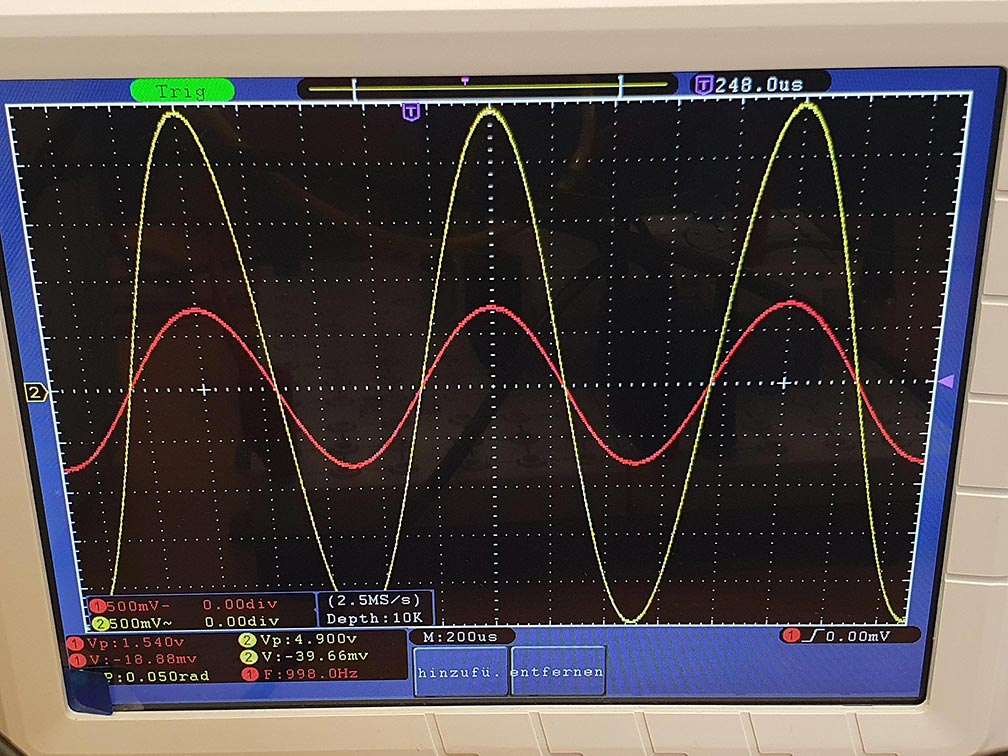
\includegraphics[width=0.4\linewidth]{nudes/messergebnisse/NichtInv1kund2.2kErgebnis.jpg}
    \caption{Oszilloskopbild des nichtinvertierenden OPVs mit $R_{2}$ = 2.2 k$\Omega$}
    \label{fig:Nichtinvertierender1k2.2kOszibild}
\end{figure}

\begin{figure}[H]
    \centering
    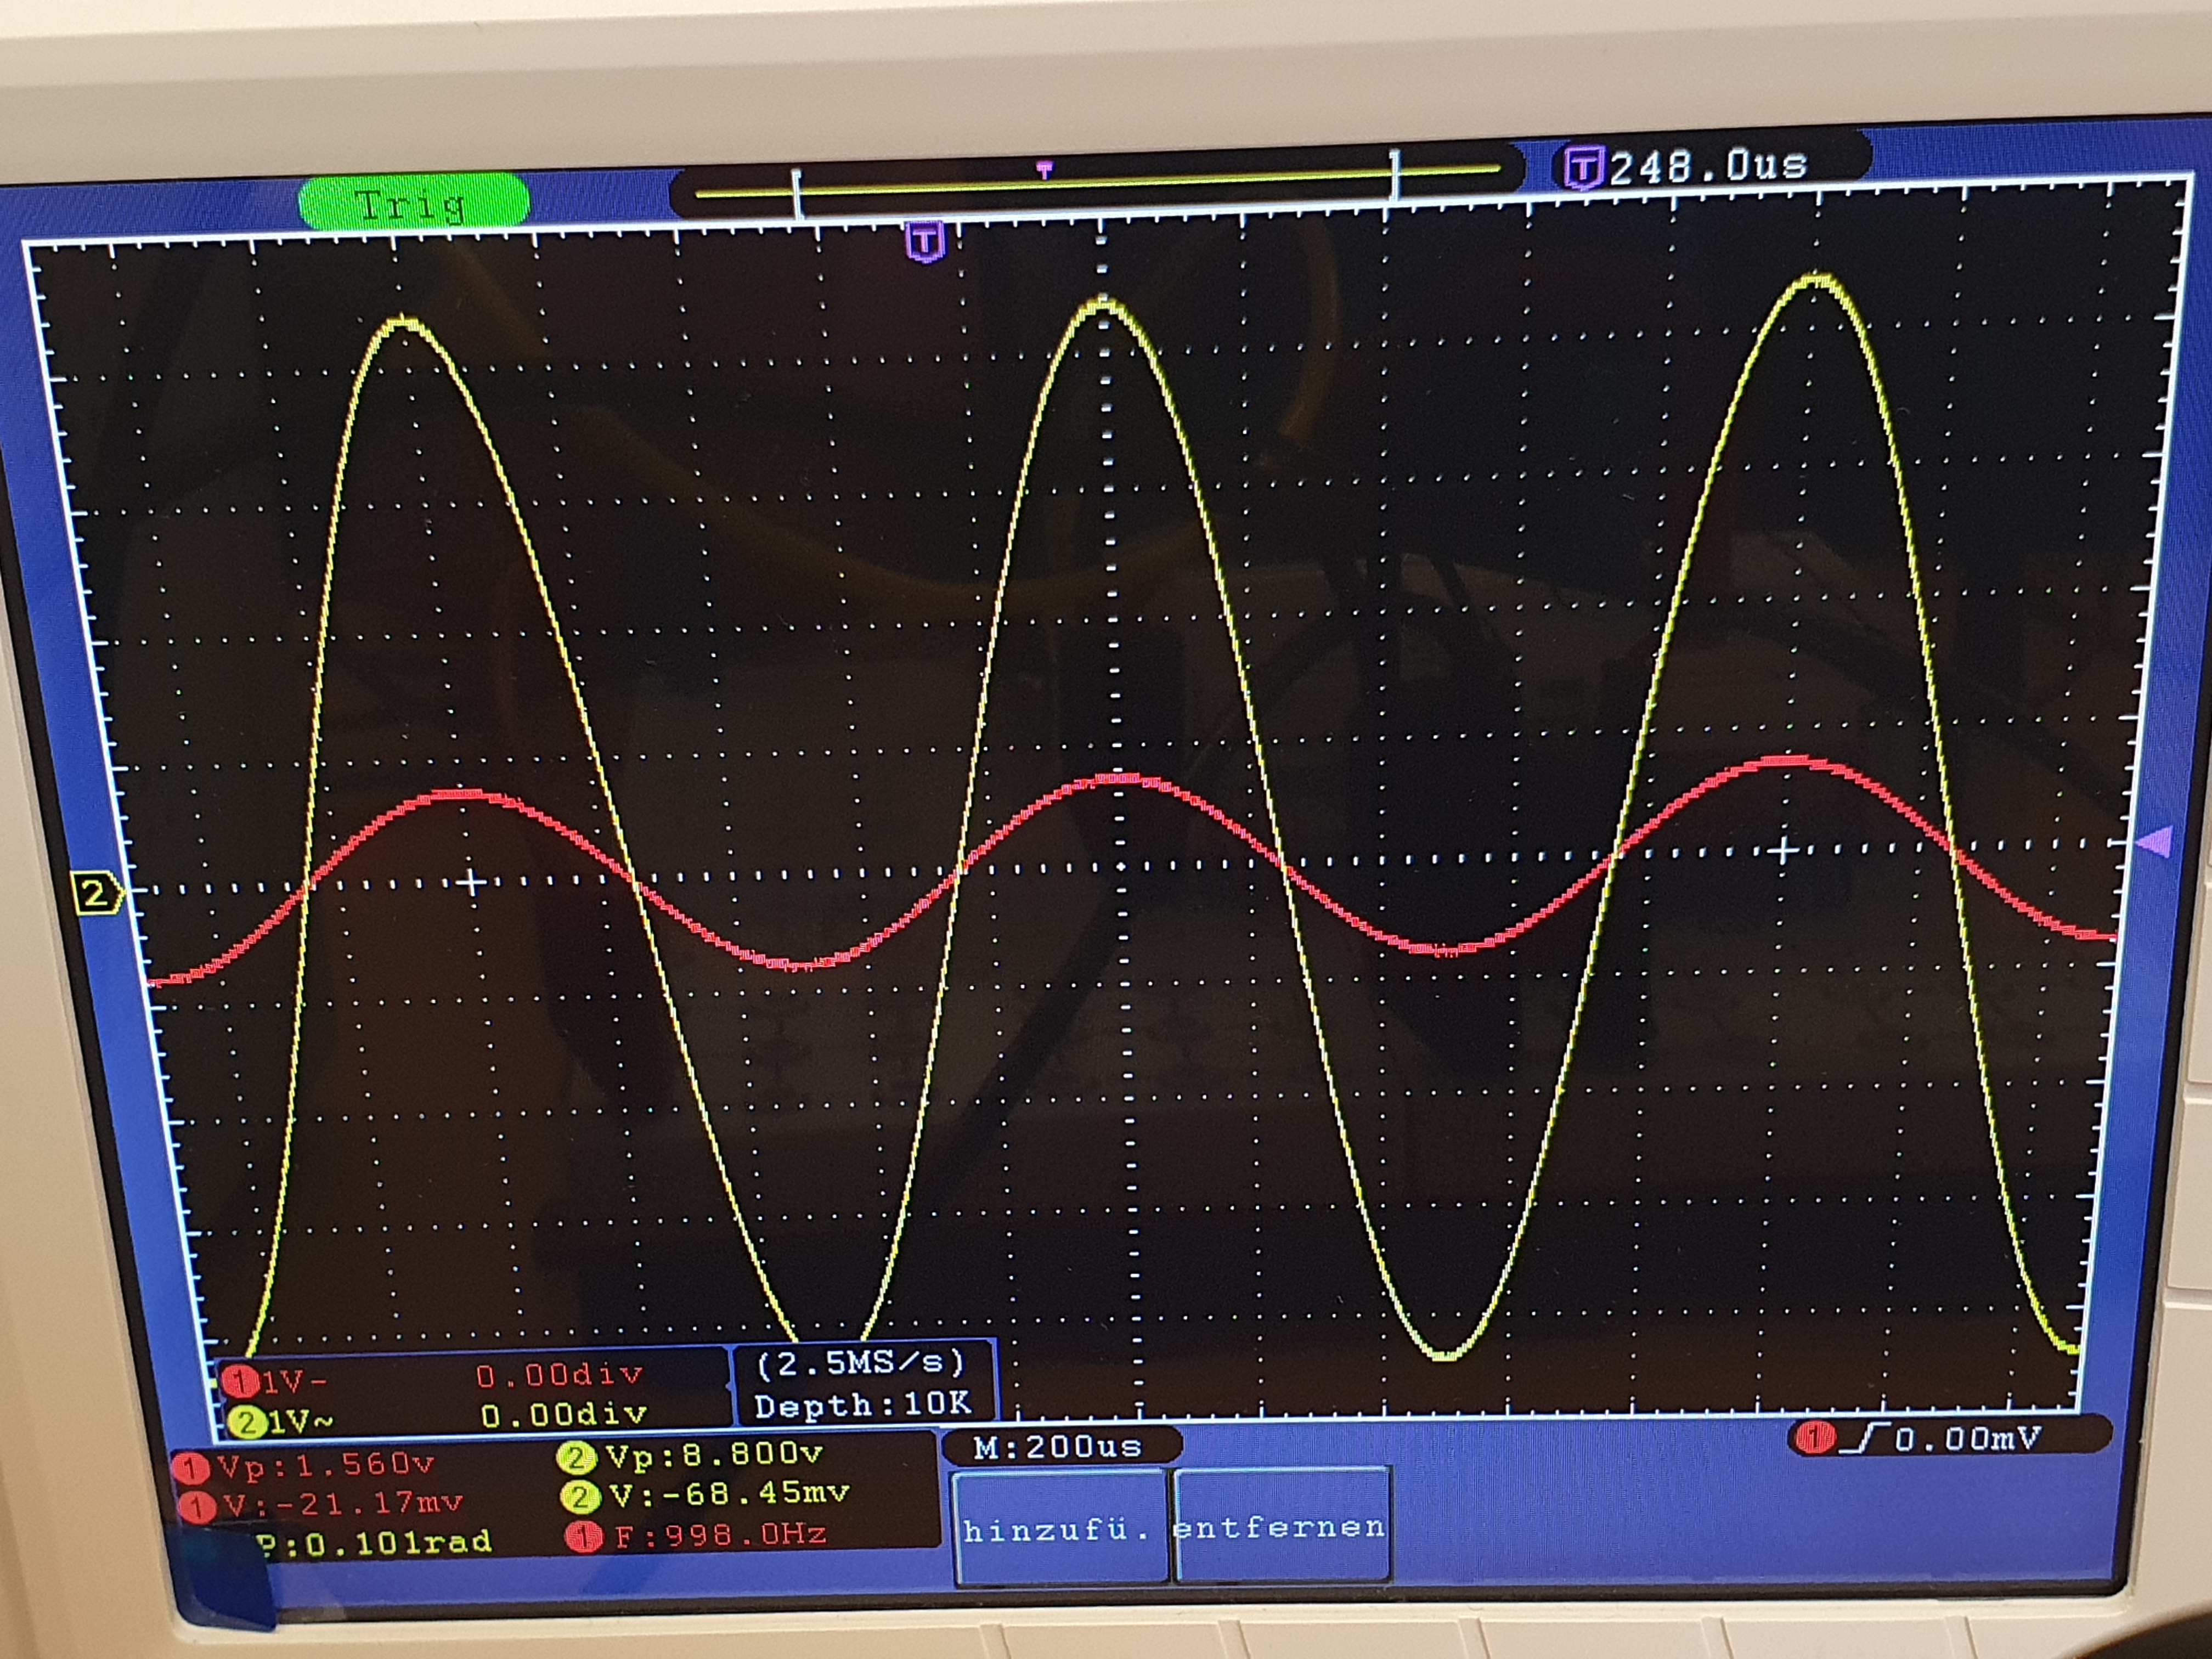
\includegraphics[width=0.4\linewidth]{nudes/messergebnisse/NichtInv1kund4.7kErgebnis.jpg}
    \caption{Oszilloskopbild des nichtinvertierenden OPVs mit $R_{2}$ = 4.7 k$\Omega$}
    \label{fig:Nichtinvertierender1k4.7kOszibild}
\end{figure}

\begin{figure}[H]
    \centering
    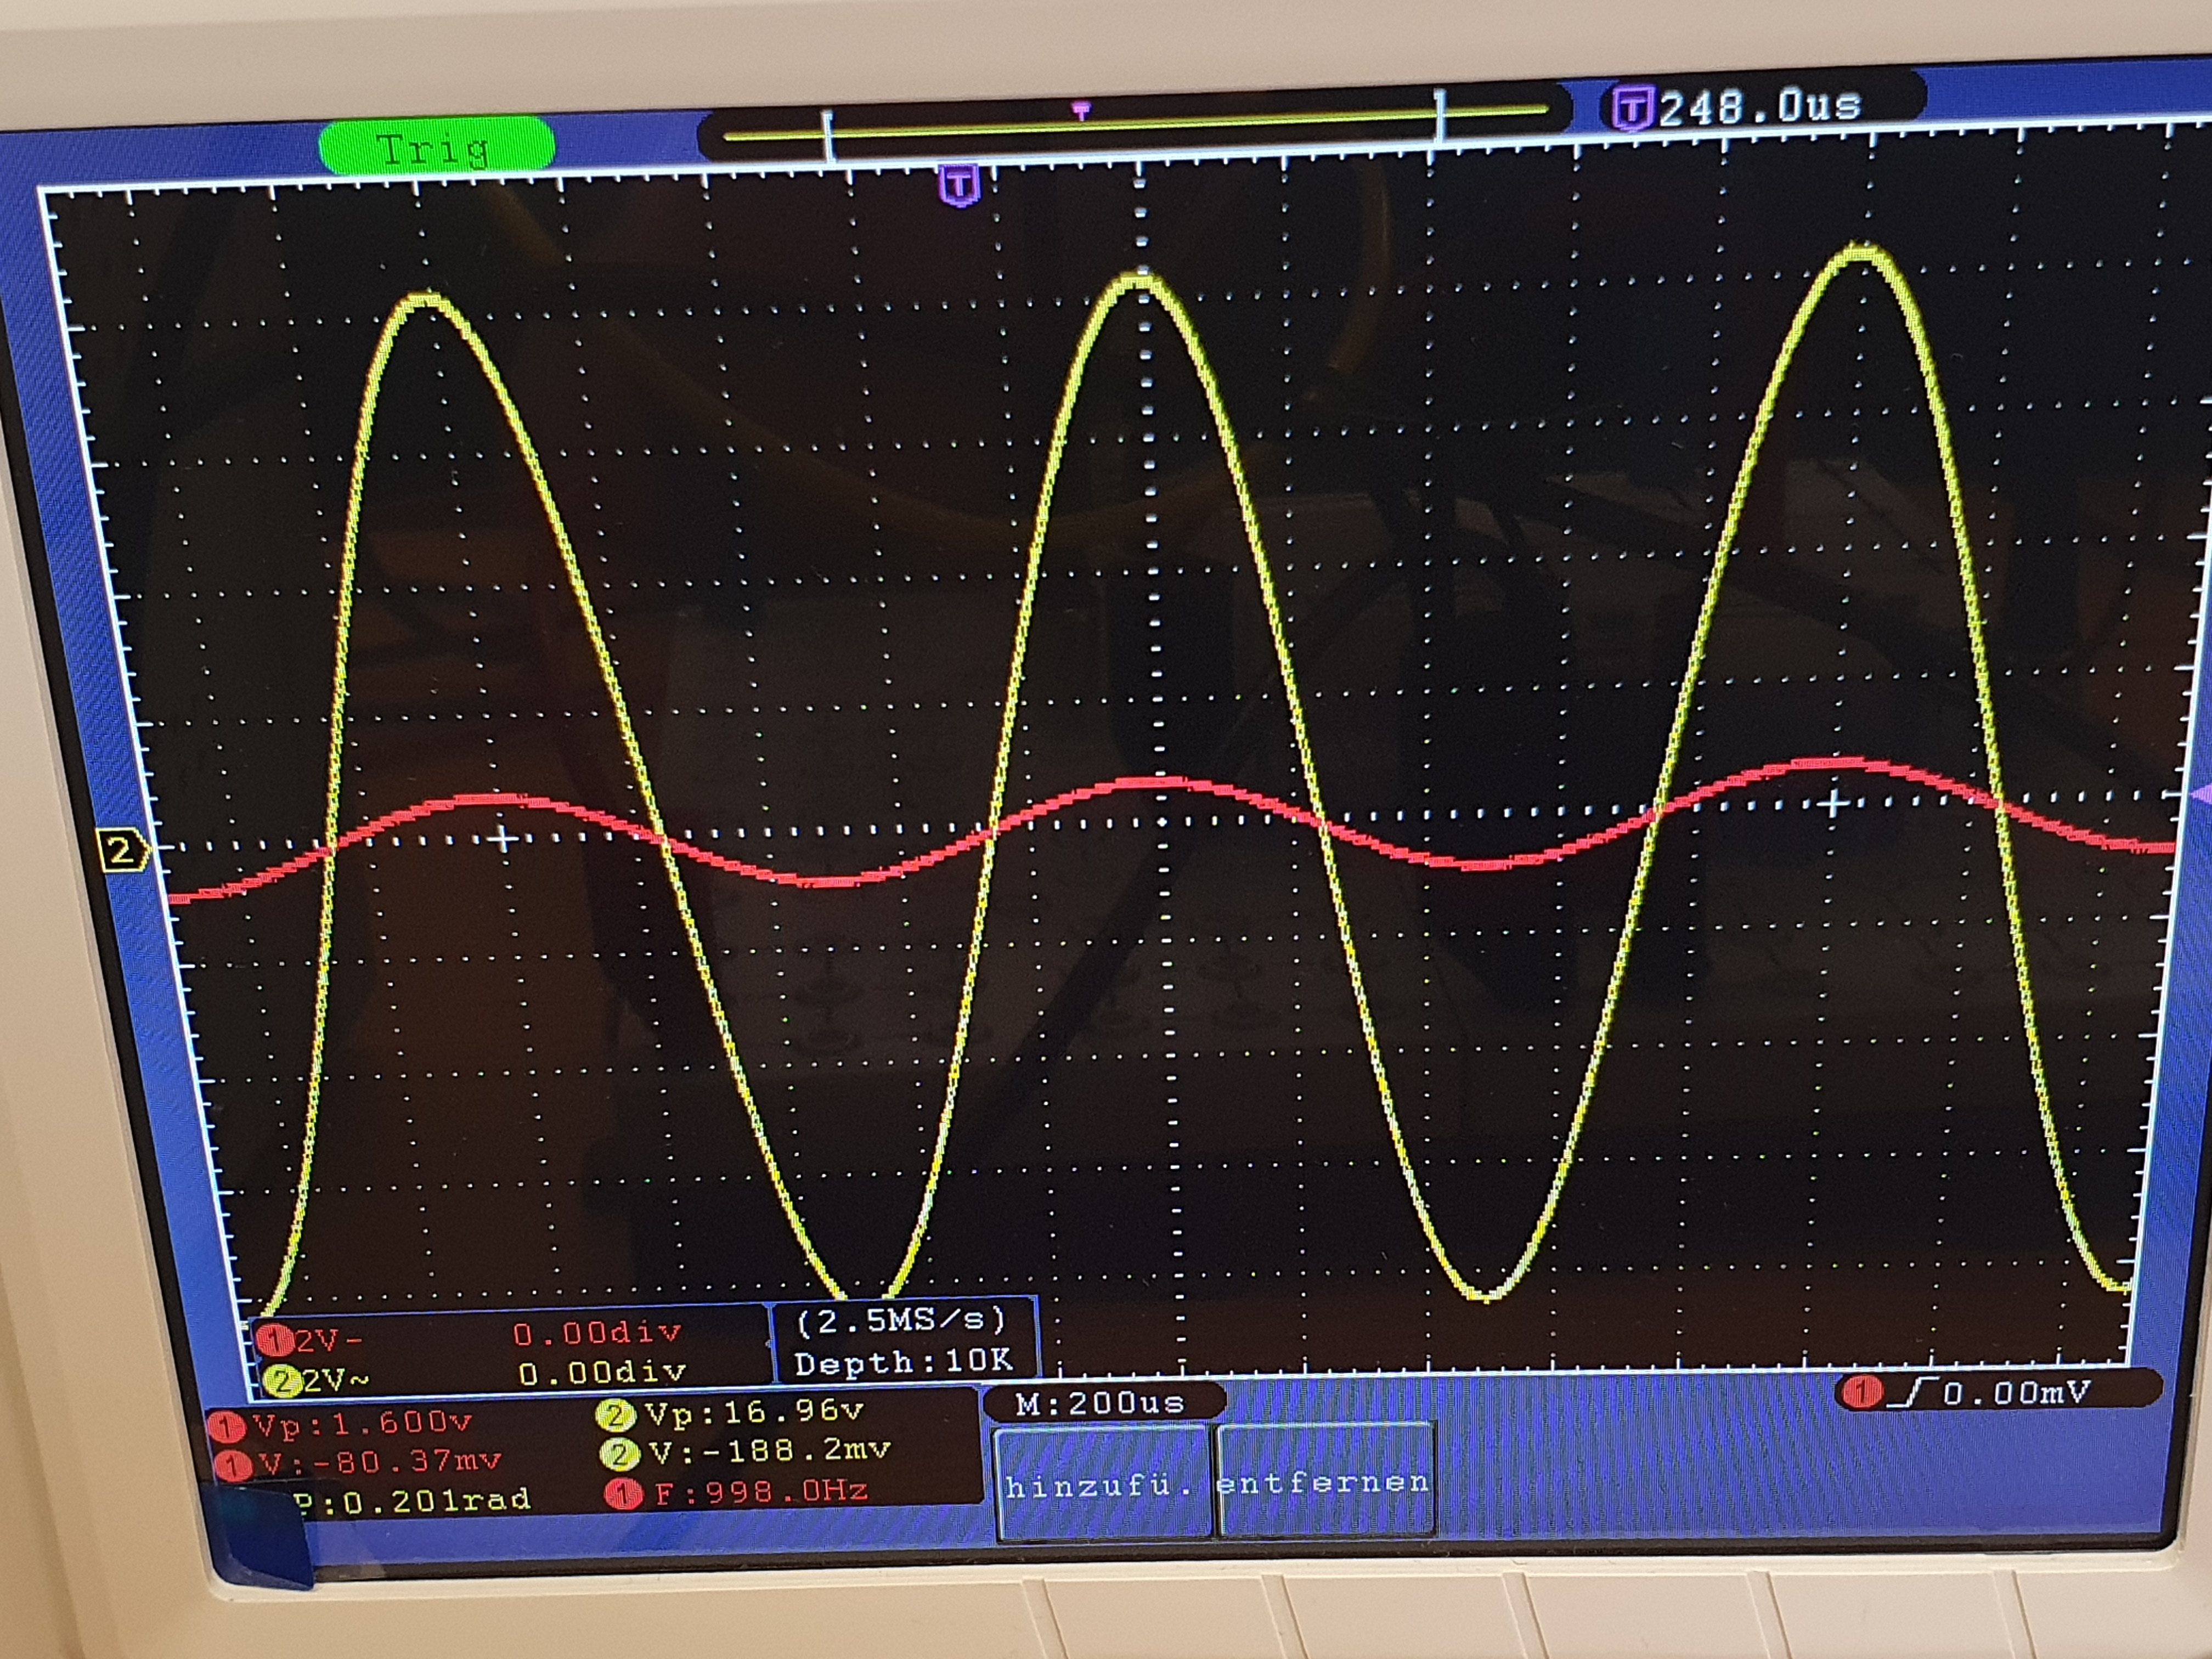
\includegraphics[width=0.4\linewidth]{nudes/messergebnisse/NichtInv1kund10kErgebnis.jpg}
    \caption{Oszilloskopbild des nichtinvertierenden OPVs mit $R_{2}$ = 10 k$\Omega$}
    \label{fig:Nichtinvertierender1k10kOszibild}
\end{figure}

\begin{table}[H]
    \centering
    \caption{Nichtinvertierender OPV Messungen}
    \label{tab:NioVerstärkungenGemessen}
    \begin{tabular}{| l | l | l | l |}
        \hline
        Nr. & $R_{2}$ / $k \Omega$ & $\frac{Kaestchen}{Kaestchen}$ $\pm$ 0.215 / & U pro Kästchen / V \\
        \hline
        1 &  0 $\pm$ 0 & $\frac{1.000}{1.000}$ & 0.500 $\pm$ 0.015 \\
        2 &  0.470 $\pm$ 0.005 & $\frac{2.200}{1.500}$ & 0.500 $\pm$ 0.015 \\
        3 &  1.500 $\pm$ 0.016 & $\frac{3.700}{1.500}$ & 0.500 $\pm$ 0.015 \\
        4 &  2.20 $\pm$  0.03  & $\frac{4.800}{1.500}$ & 0.500 $\pm$ 0.015 \\
        5 &  4.70 $\pm$  0.05  & $\frac{4.400}{0.700}$ & 1.00 $\pm$ 0.03 \\
        6 & 10.00 $\pm$  0.1   & $\frac{4.100}{0.400}$ & 2.00 $\pm$ 0.06 \\
        \hline
    \end{tabular}
\end{table}


\subsection{Differenzierer}

Mit dem Differenzierer, aufgebaut laut Abbildungen \ref{fig:SchaltungDifferenzierer}, wurde es nun etwas spannender und komplexer. 
Durch den eingebauten Kondensator am Eingang des OPVs kann die Schaltung tatsächlich dazu verwendet werden, eingehende Funktionen abzuleiten. 
Um dies in Realität nachweißen zu können, wurde ein Eingangssignal mit 0.1 V Rechteck mit 500 Hz an die Schaltung angelegt. Zunächst wurden als Widerstand $R_{1}$ 0 k$\Omega$, als R 10 K$\Omega$ und als Kapazität 1 $mu$F gewählt.
Das daraus folgende Oszilloskopbild lässt sich in nachfolgender Abbildung \ref{fig:Differenzierer0R1} erkennen.

\begin{figure}[H]
    \centering
    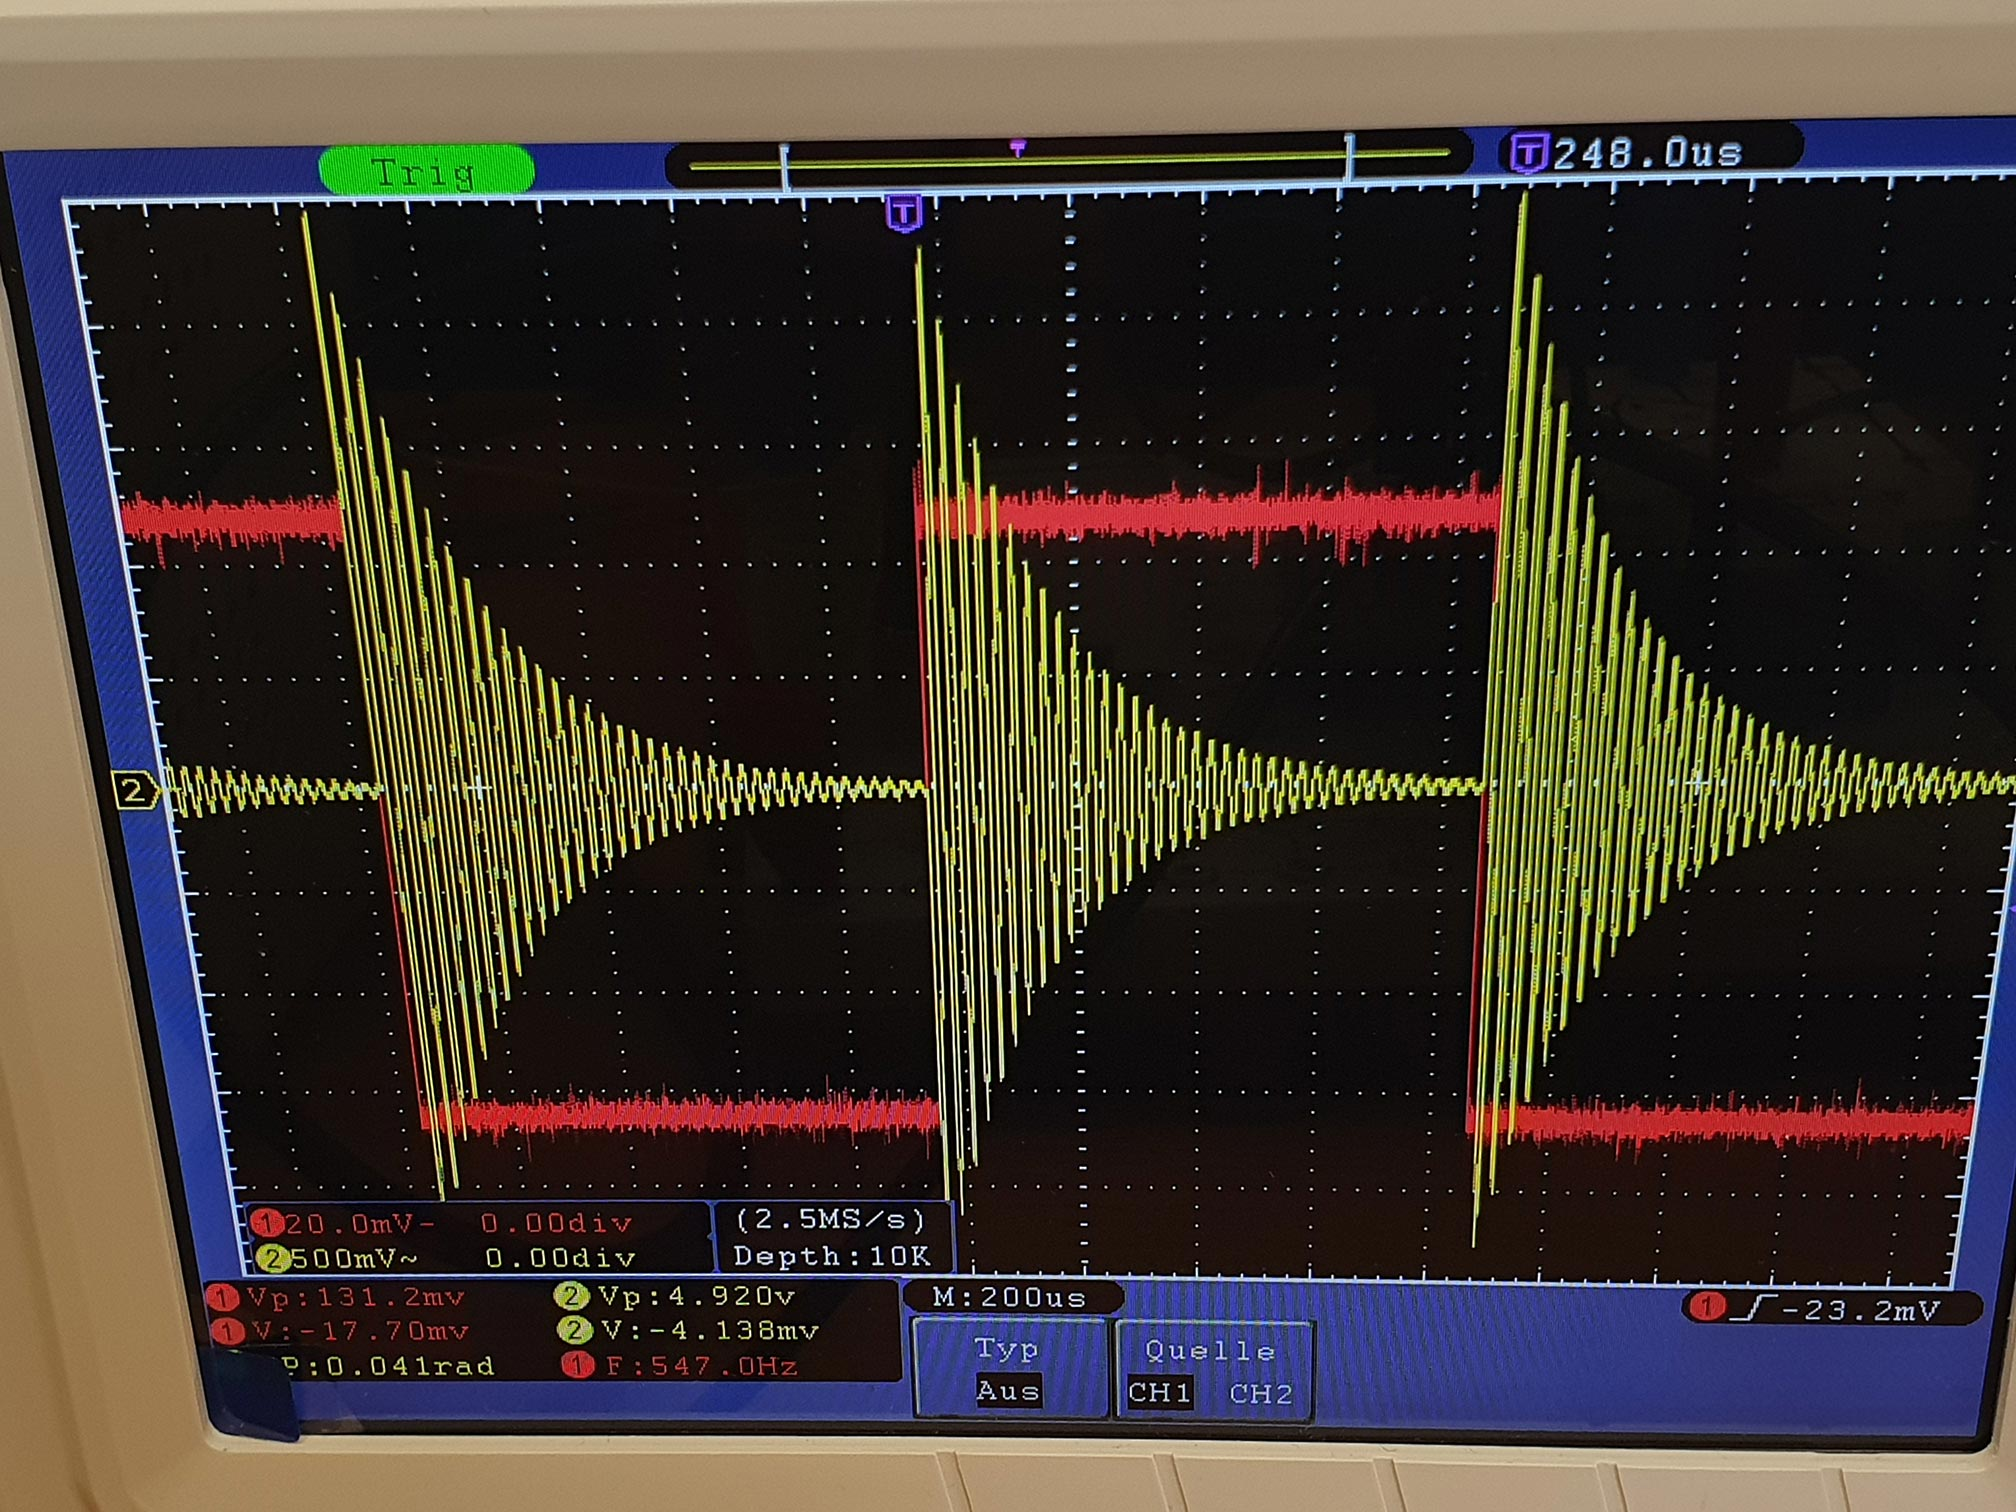
\includegraphics[width=0.4\linewidth]{nudes/messergebnisse/DifferenziererOhneEingangsR.jpg}
    \caption{Differenzierer ohne Eingangswiderstand}
    \label{fig:Differenzierer0R1}
\end{figure}

\noindent
Nun soll der Eingangswiderstand $R_{1}$ auf 1 k$\Omega$ und die Kapazität auf 10 nF verändert werden. Daraus resultierte folgendes Oszilloskopbild:

\begin{figure}[H]
    \centering
    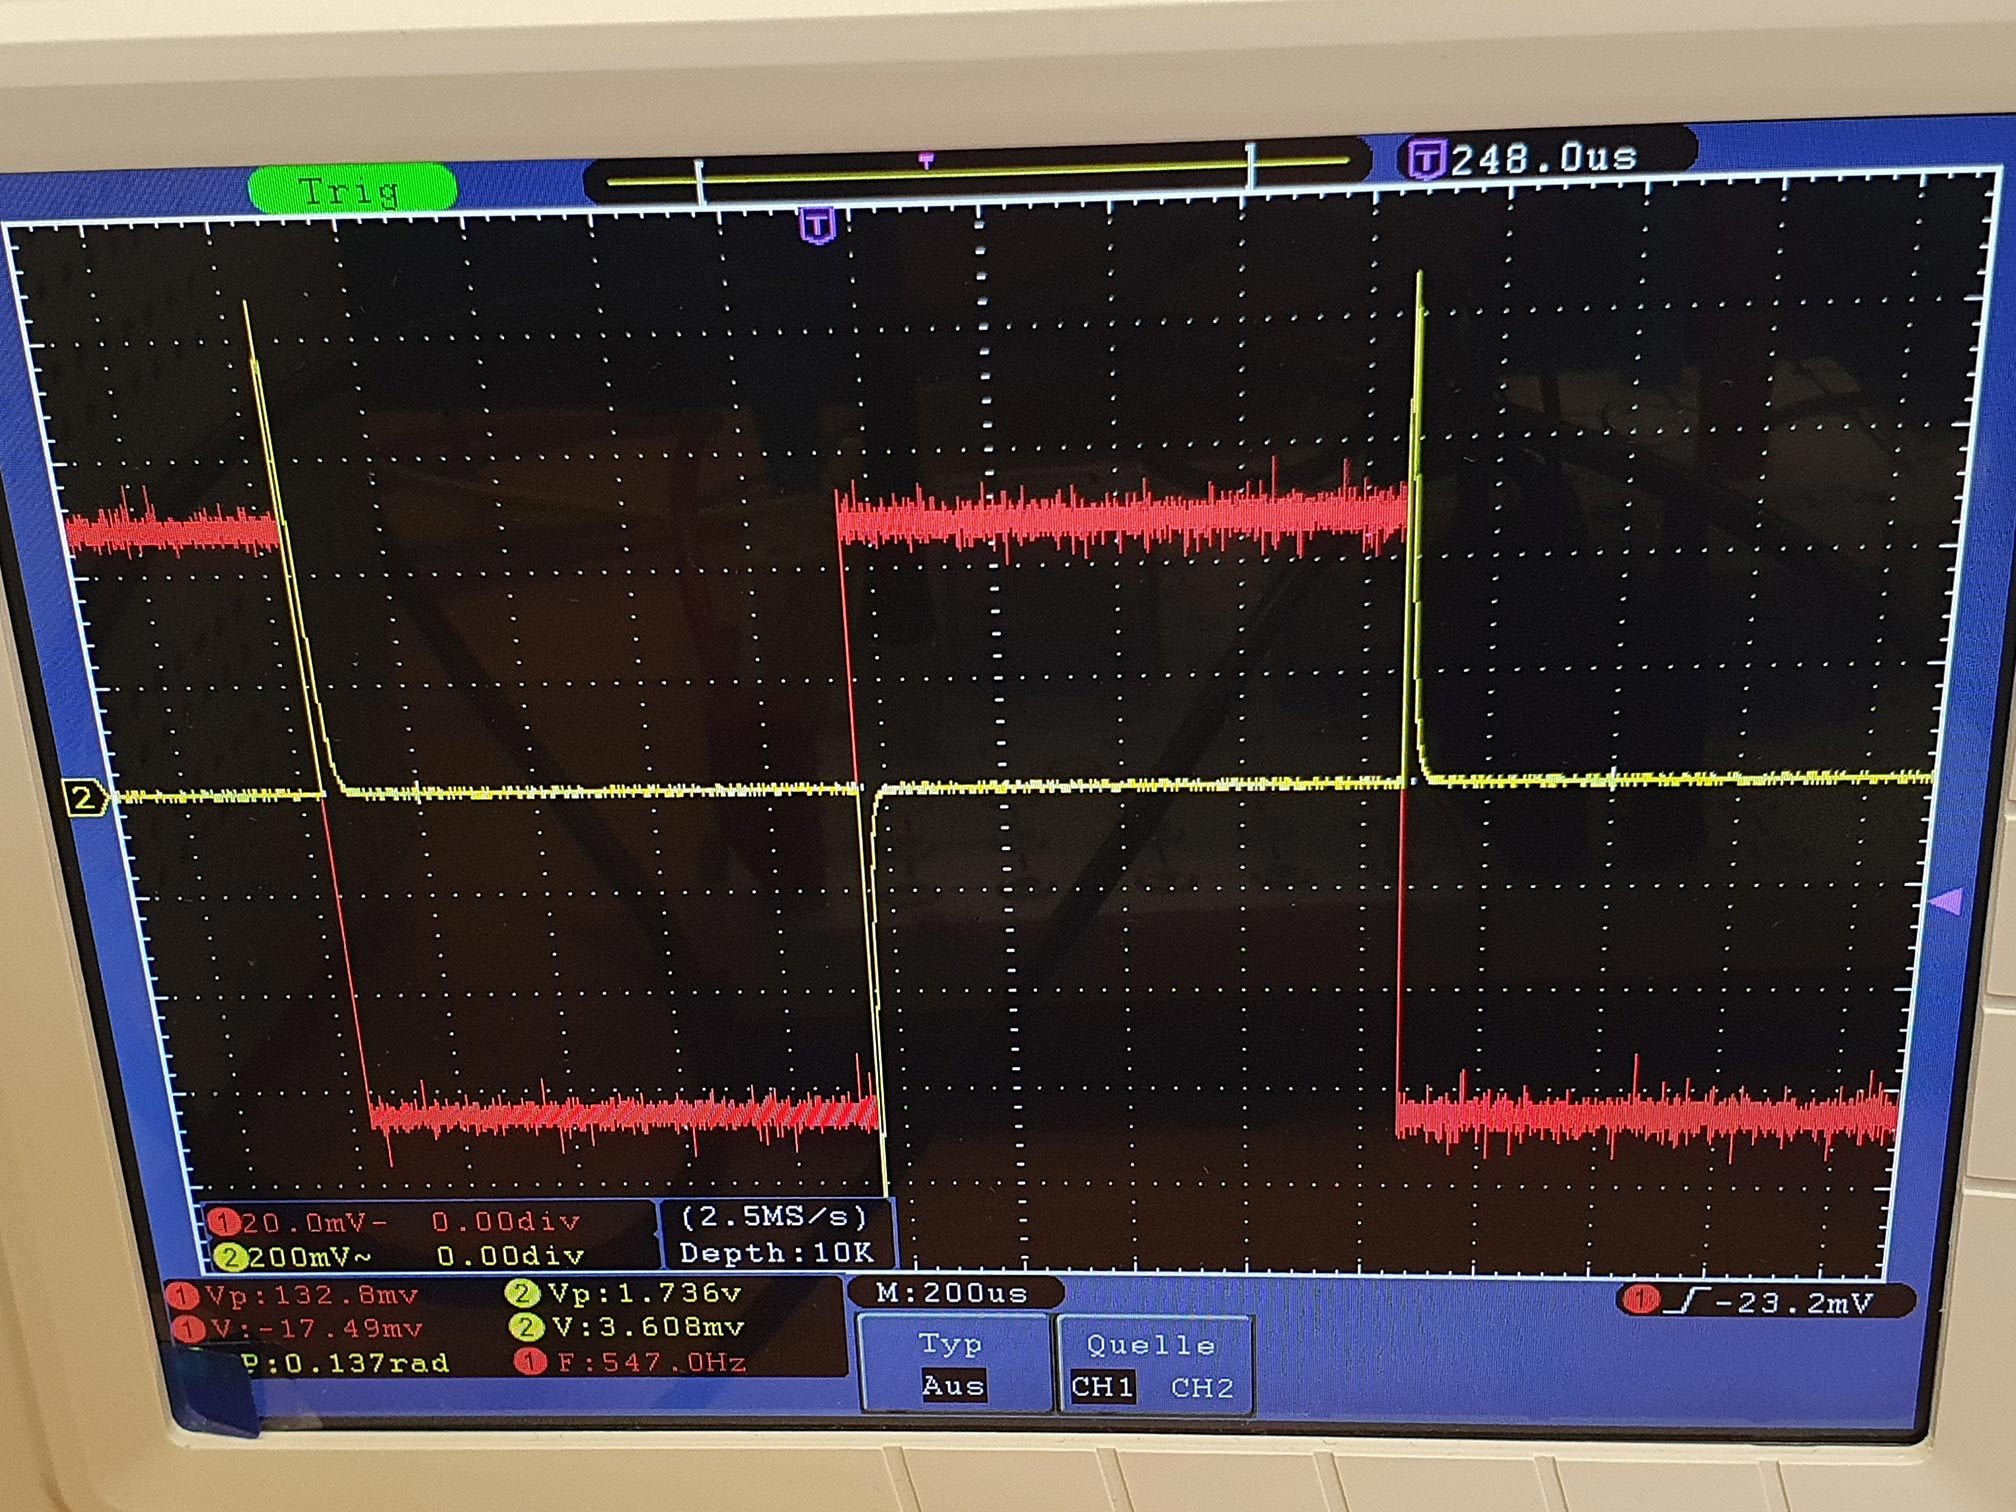
\includegraphics[width=0.4\linewidth]{nudes/messergebnisse/DifferenziererMitEingangsR.jpg}
    \caption{Differenzierer mit Eingangswiderstand 1 k$\Omega$}
    \label{fig:Differenzierer1R1}
\end{figure}

\noindent
Außerdem wurde selber Prozess noch mit einer Sinusspannung und einer Dreiecksspannung ausprobiert. Die Frequenz wurde hierfür auf 500 Hz gestellt.

\begin{figure}[H]
    \centering
    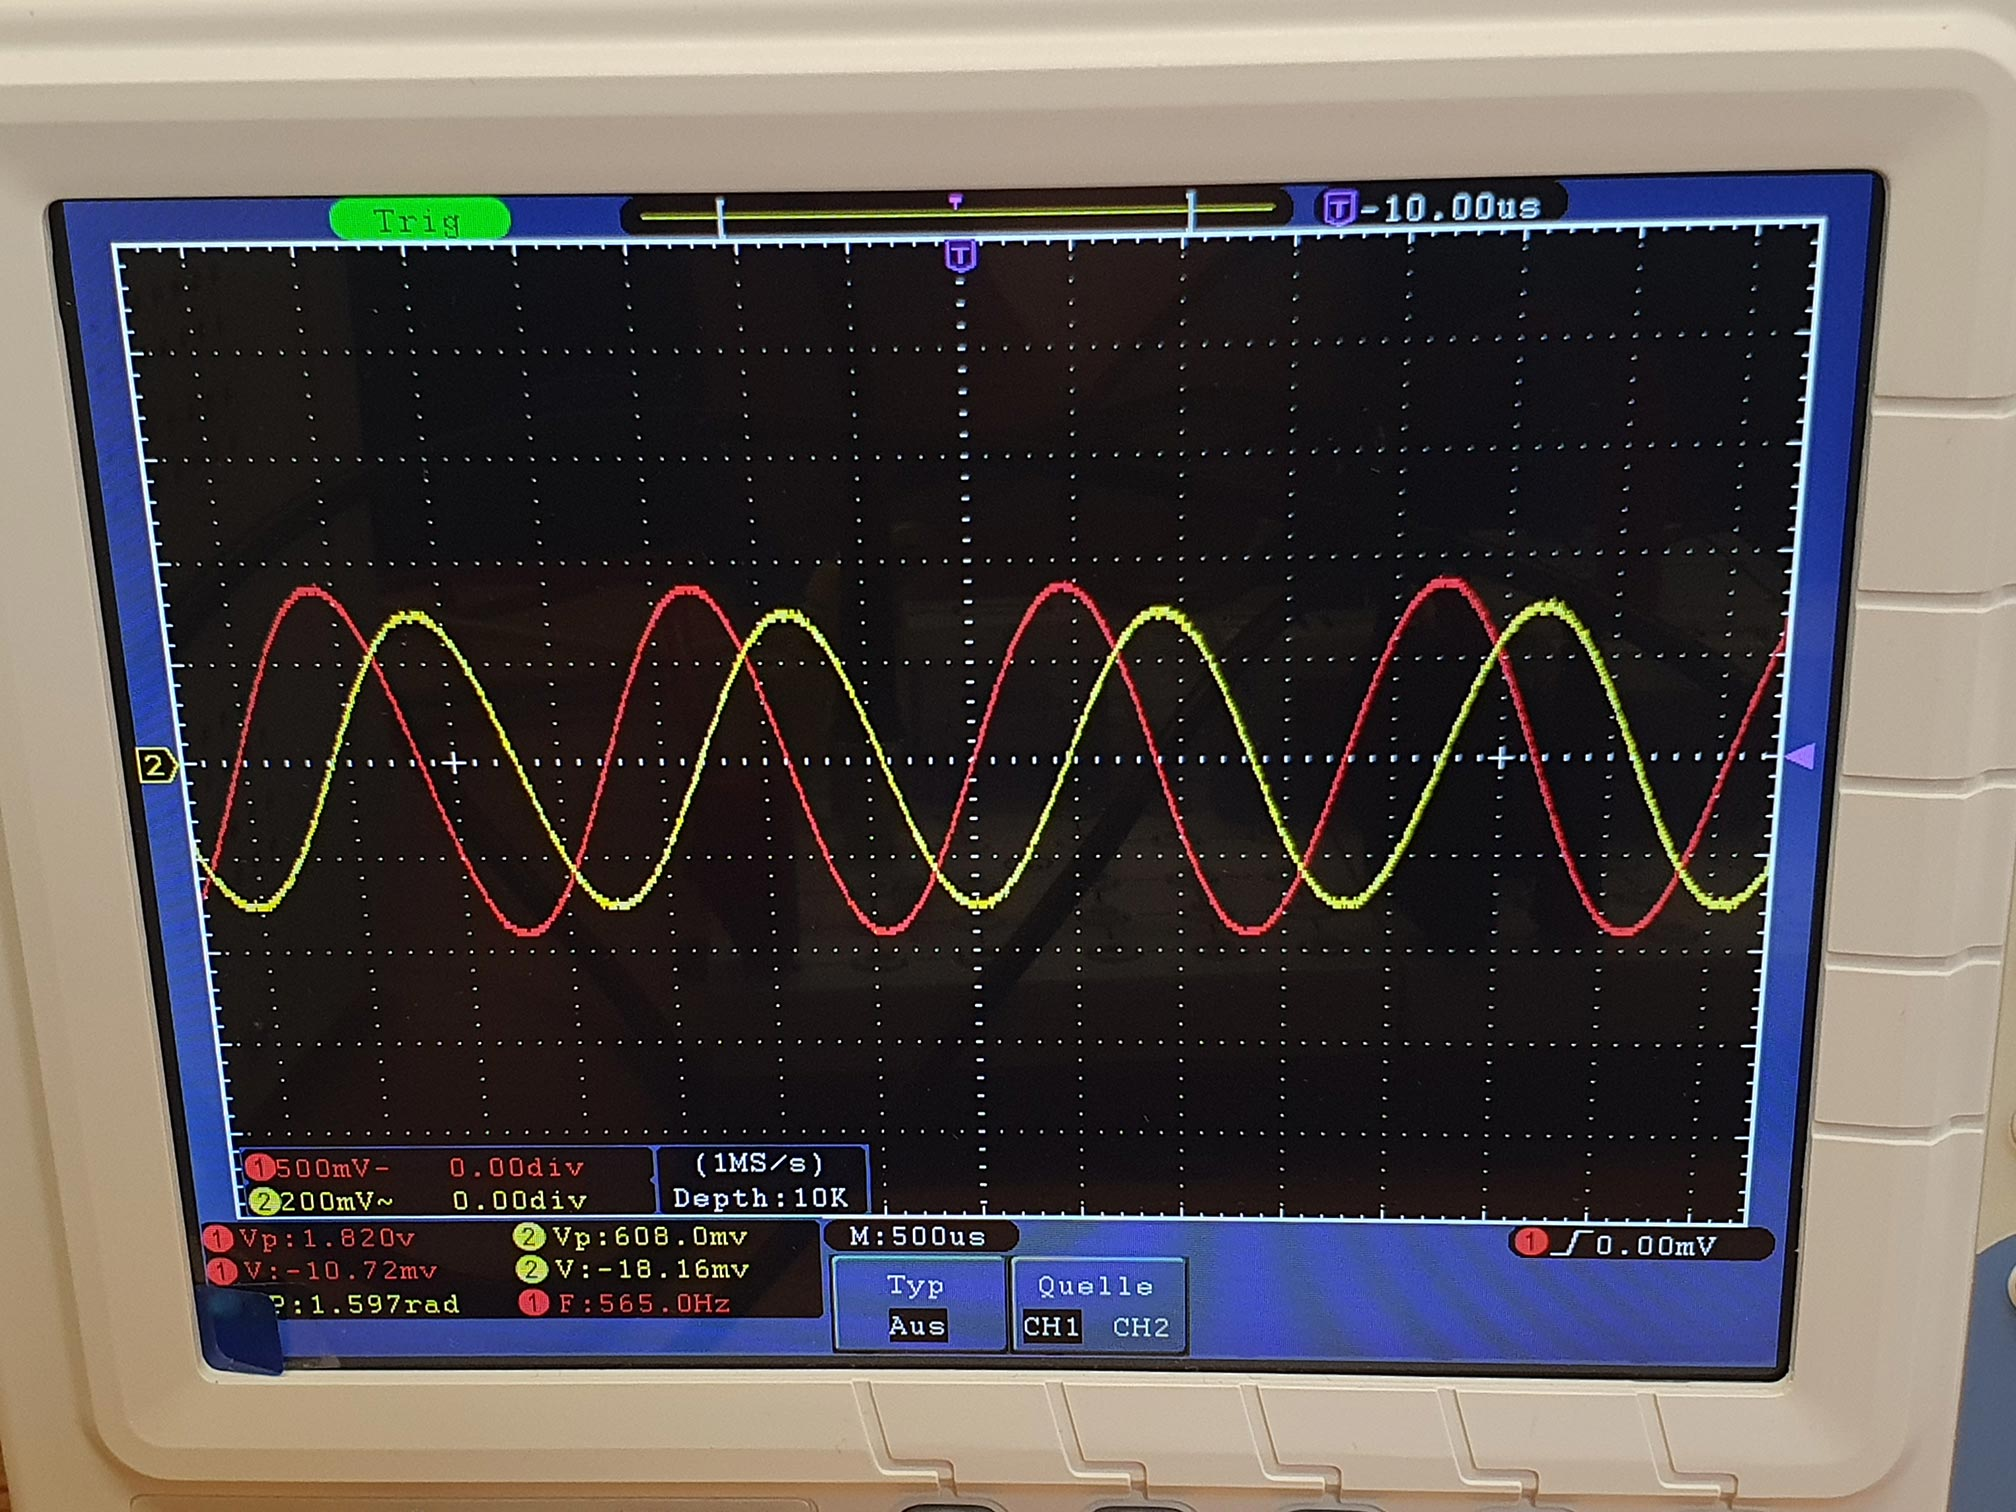
\includegraphics[width=0.4\linewidth]{nudes/messergebnisse/DifferenziererSinus.jpg}
    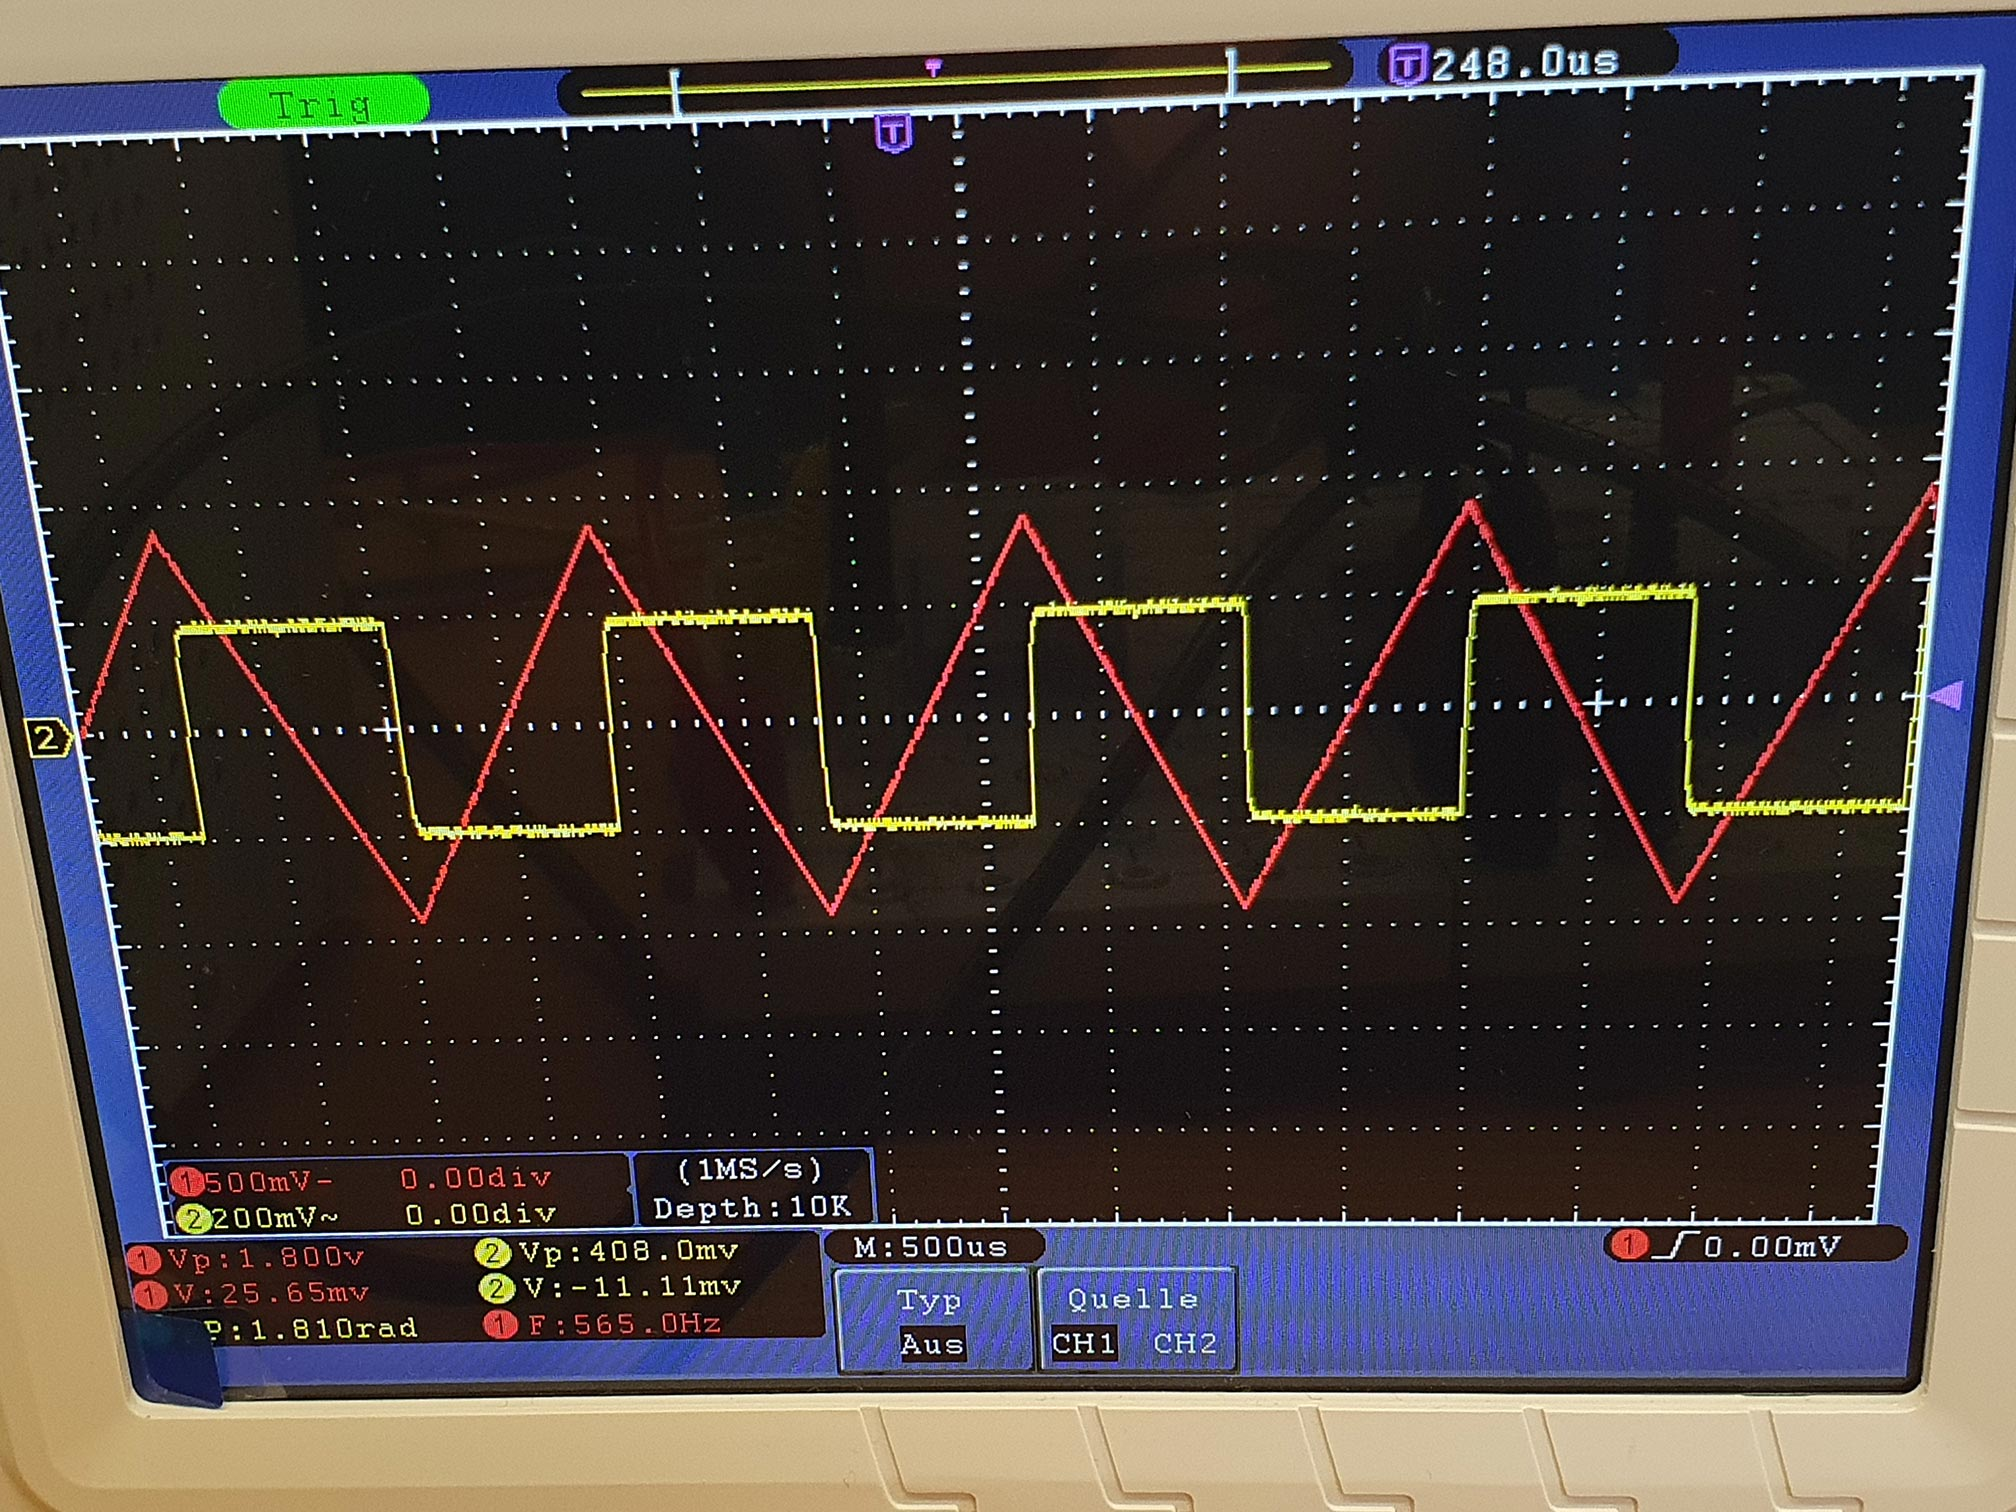
\includegraphics[width=0.4\linewidth]{nudes/messergebnisse/DifferenziererDreieck.jpg}
    \caption{Differenzierer mit Eingangswiderstand 1 k$\Omega$ Sinus/Dreieck}
    \label{fig:Differenzierer1R1Sinus/Dreieck}
\end{figure}


\subsection{Integrierer}
Zum Schluss wurde der Versuch Operationsverstärker mit einer Schaltung zur Integration laut Abbildungen \ref{fig:SchaltungIntegrierer} abgerundet. Hierfür wurde der Kondensator nicht mehr beim Eingangssignal angeschlossen, sondern paralell zum Widerstand R.
Die verwendeten Utensilien waren zum einen ein 10 nF Kondensator, ein 1 M$\Omega$ Widerstand R und ein 10 k$\Omega$ Widerstand $R_{1}$. Betrieben wurde die Schaltung mit einer rechteckigen Wechselspannung von 2 V mit einer Frequenz von 1 kHz. Als Ergebniss dient wiederum ein Oszilloskopbild.

\begin{figure}[H]
    \centering
    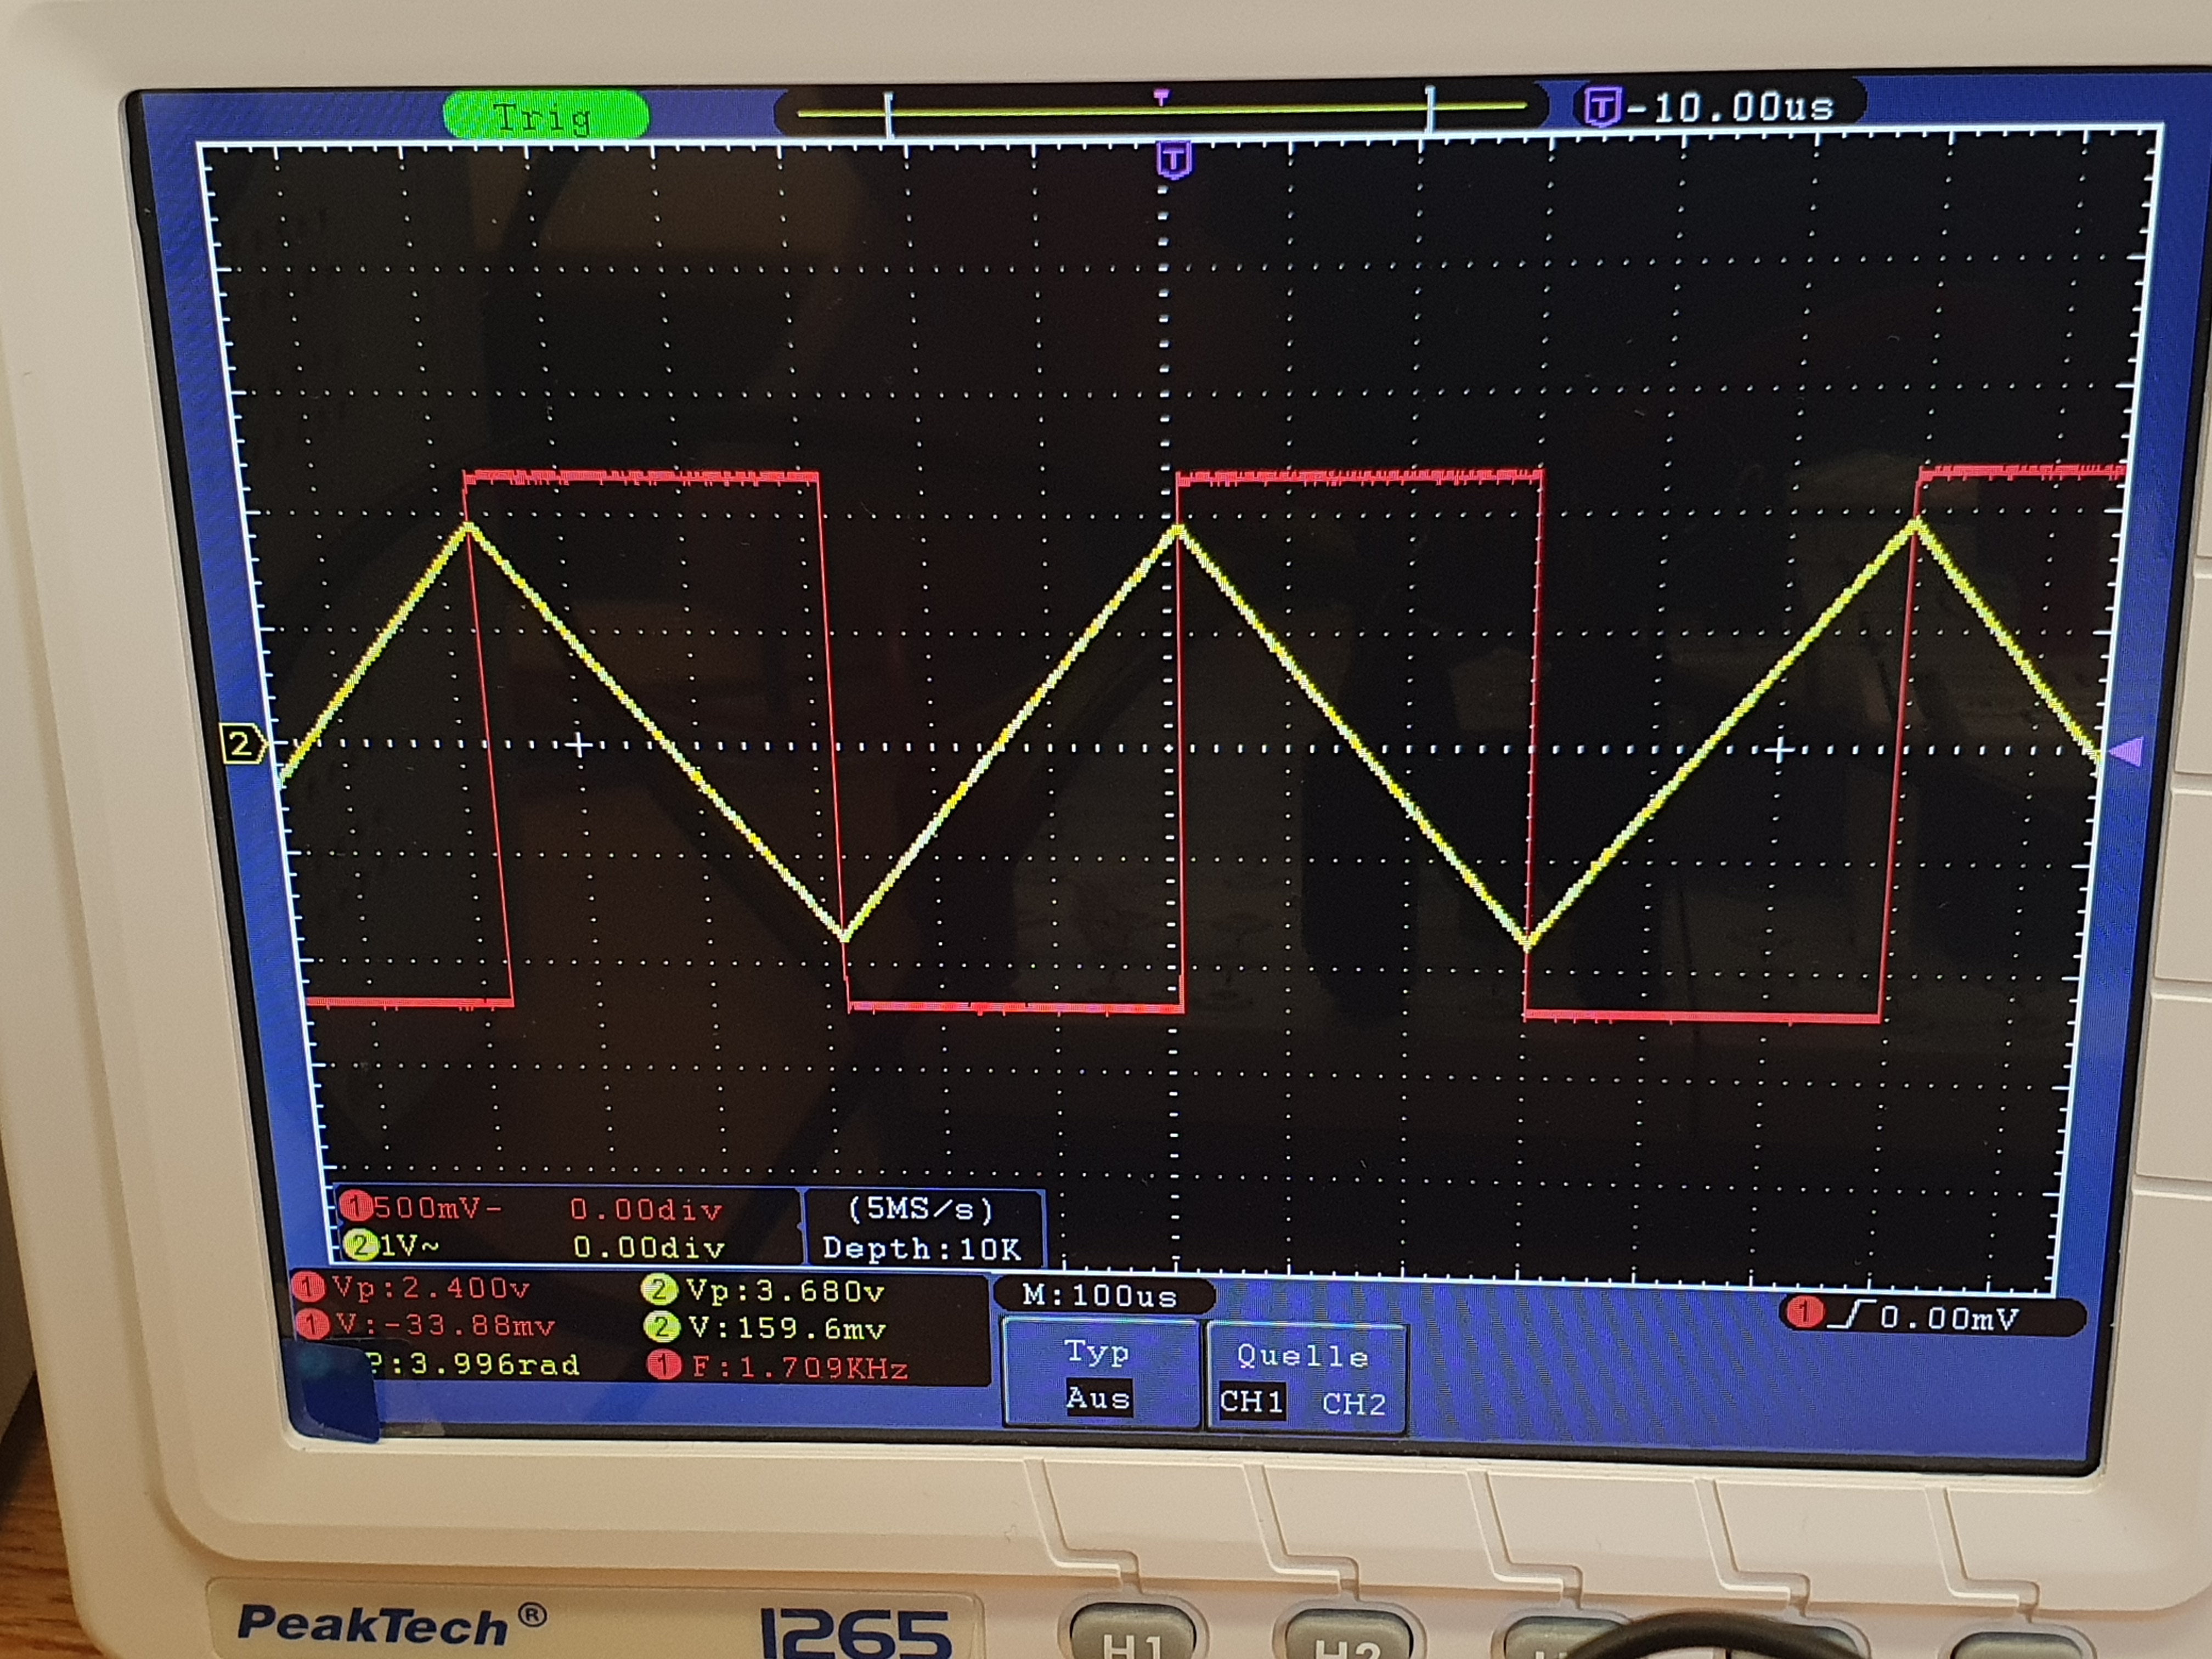
\includegraphics[width=0.4\linewidth]{nudes/messergebnisse/IntegriererRechteck10nF.jpg}
    \caption{Integrierer 10 nF}
    \label{fig:IntegriererResultat1}
\end{figure}

\noindent
Danach wurde der Kondensator von 10 nF auf 2.2 nF verändert und die Eingangsspannung auf 200 mV mit 100 Hz gesetzt. Das resultierende Oszilloskopbild sieht wie folgt aus:

\begin{figure}[H]
    \centering
    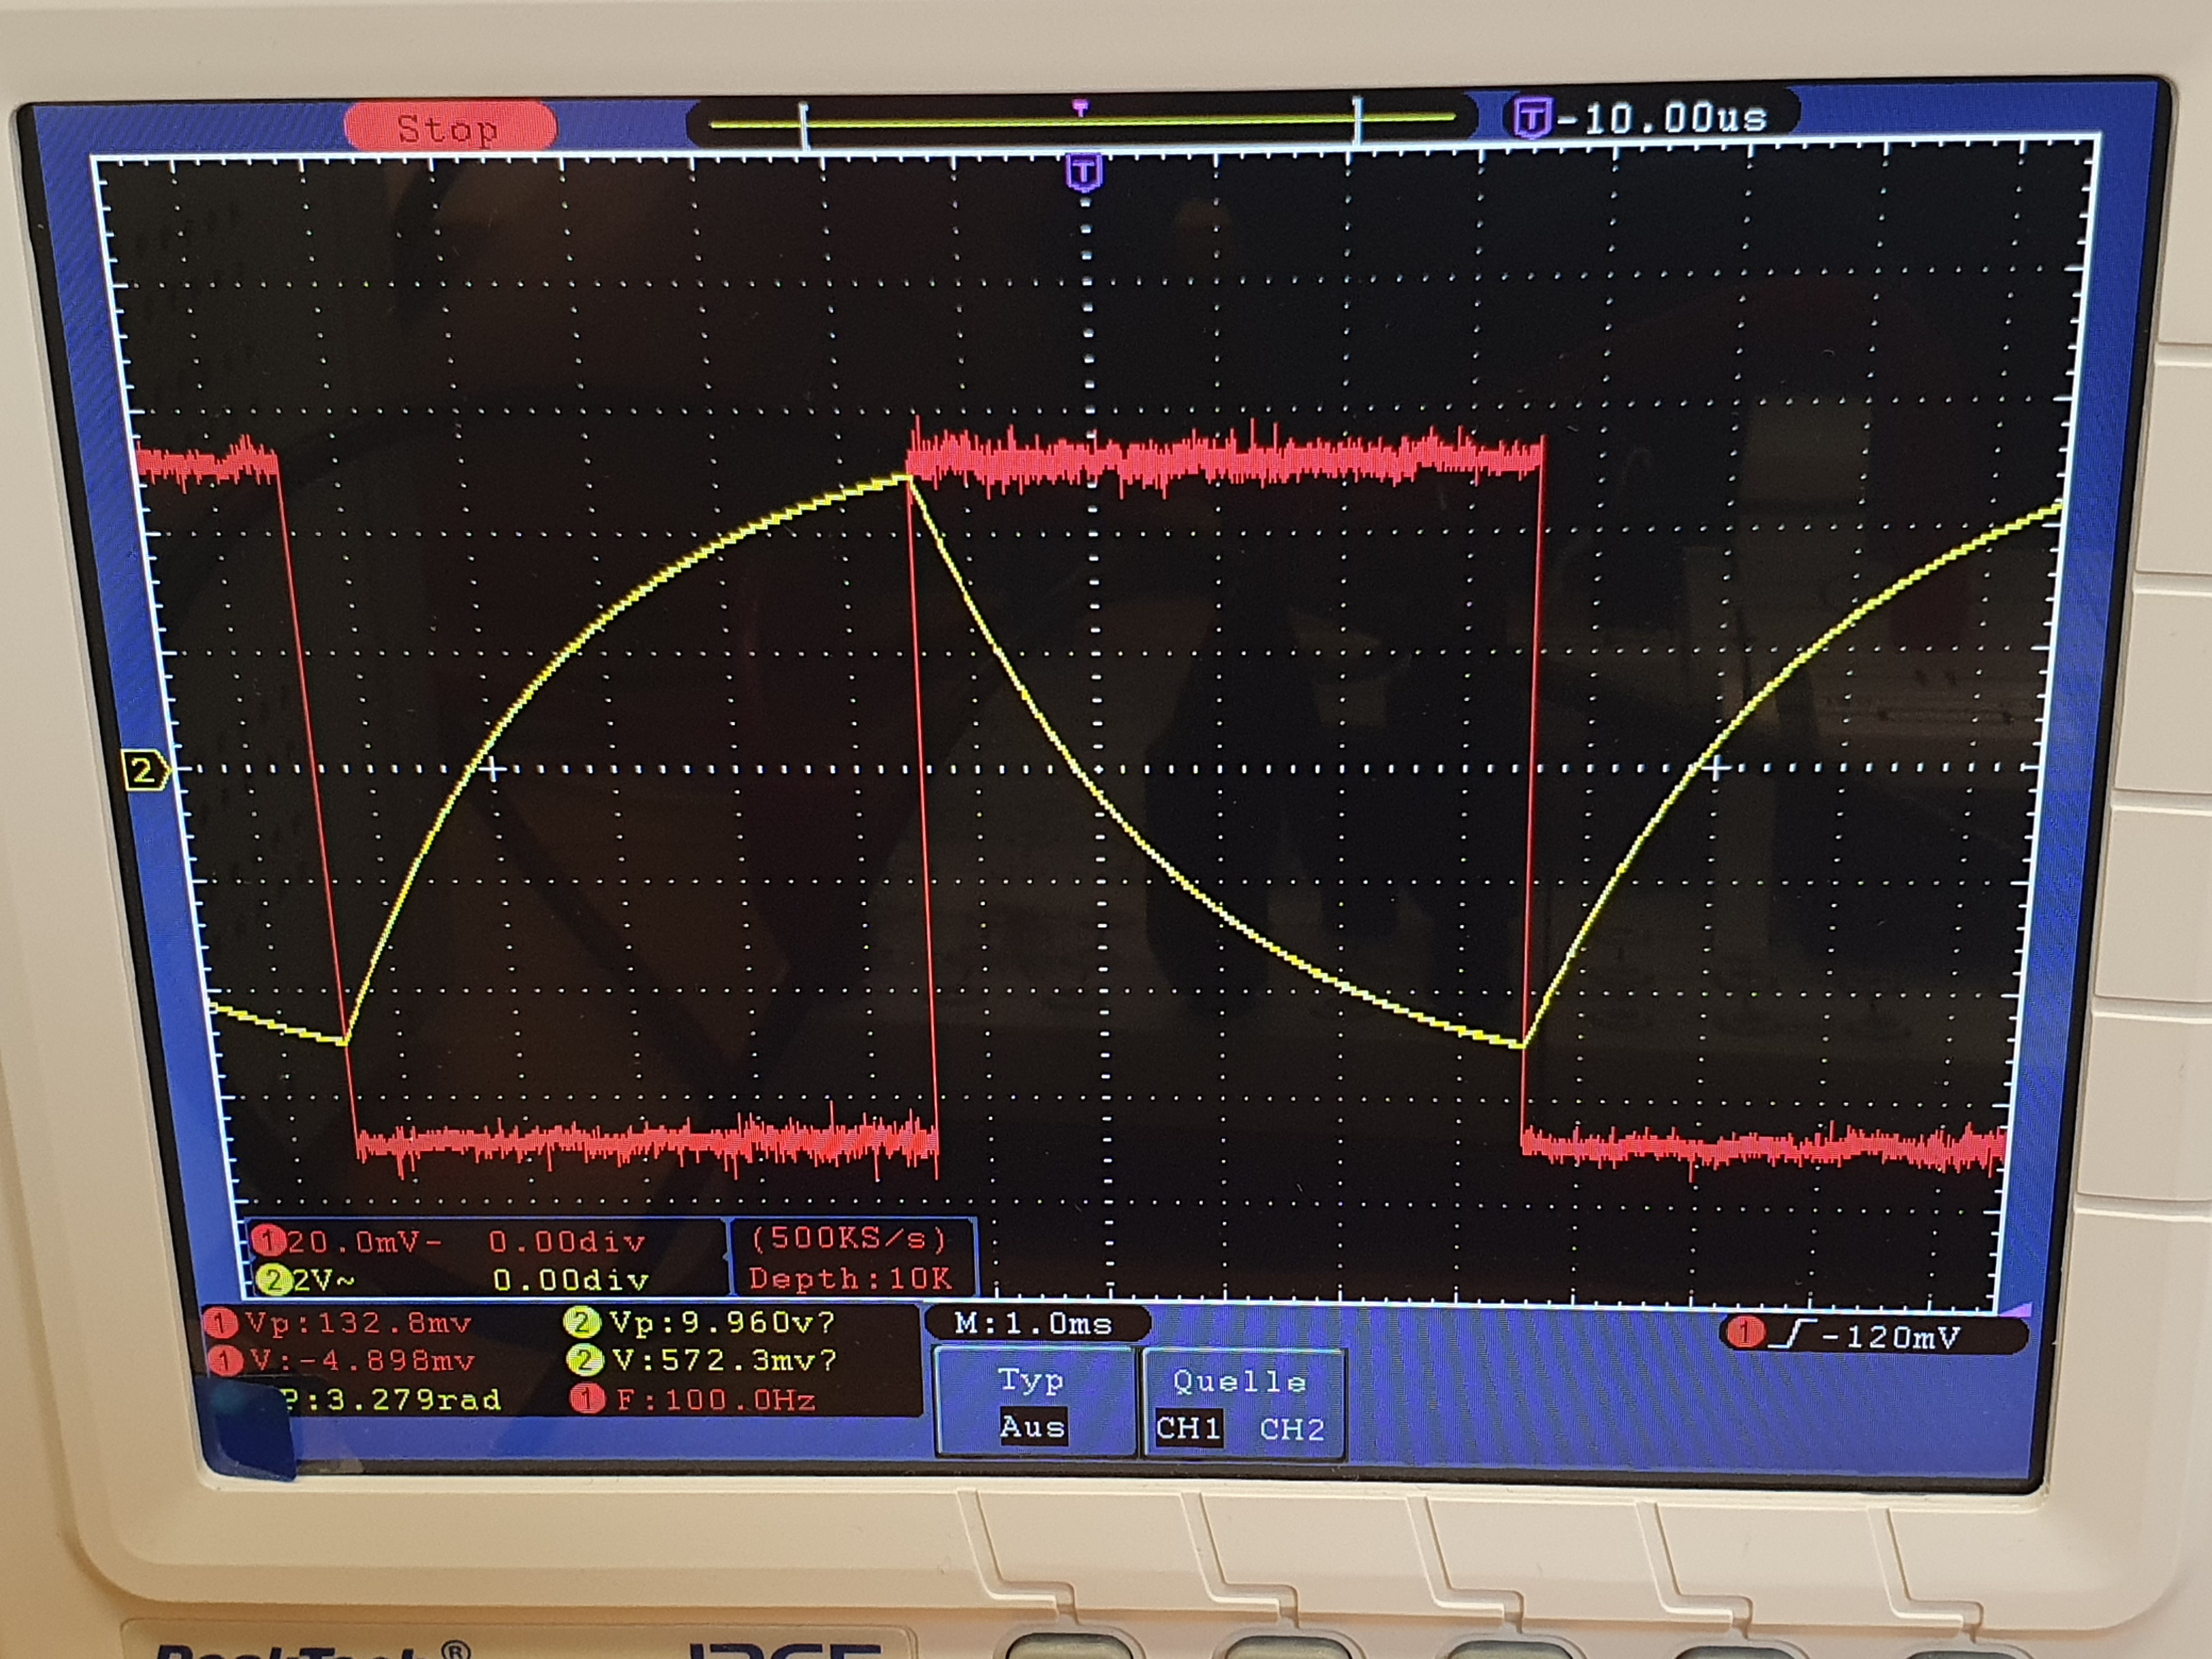
\includegraphics[width=0.4\linewidth]{nudes/messergebnisse/IntegriererRechteck2.2.jpg}
    \caption{Integrierer 2.2 nF}
    \label{fig:IntegriererResultat2}
\end{figure}

\noindent
Am Ende wurd nun noch selbiges für Sinus- und Dreiecksspannungen durchgeführt. Dabei wurde das Eingangssignal auf 2 V mit 1 kHz gesetzt und die Ergebnisse als Oszilloskopbilder exportiert.

\begin{figure}[H]
    \centering
    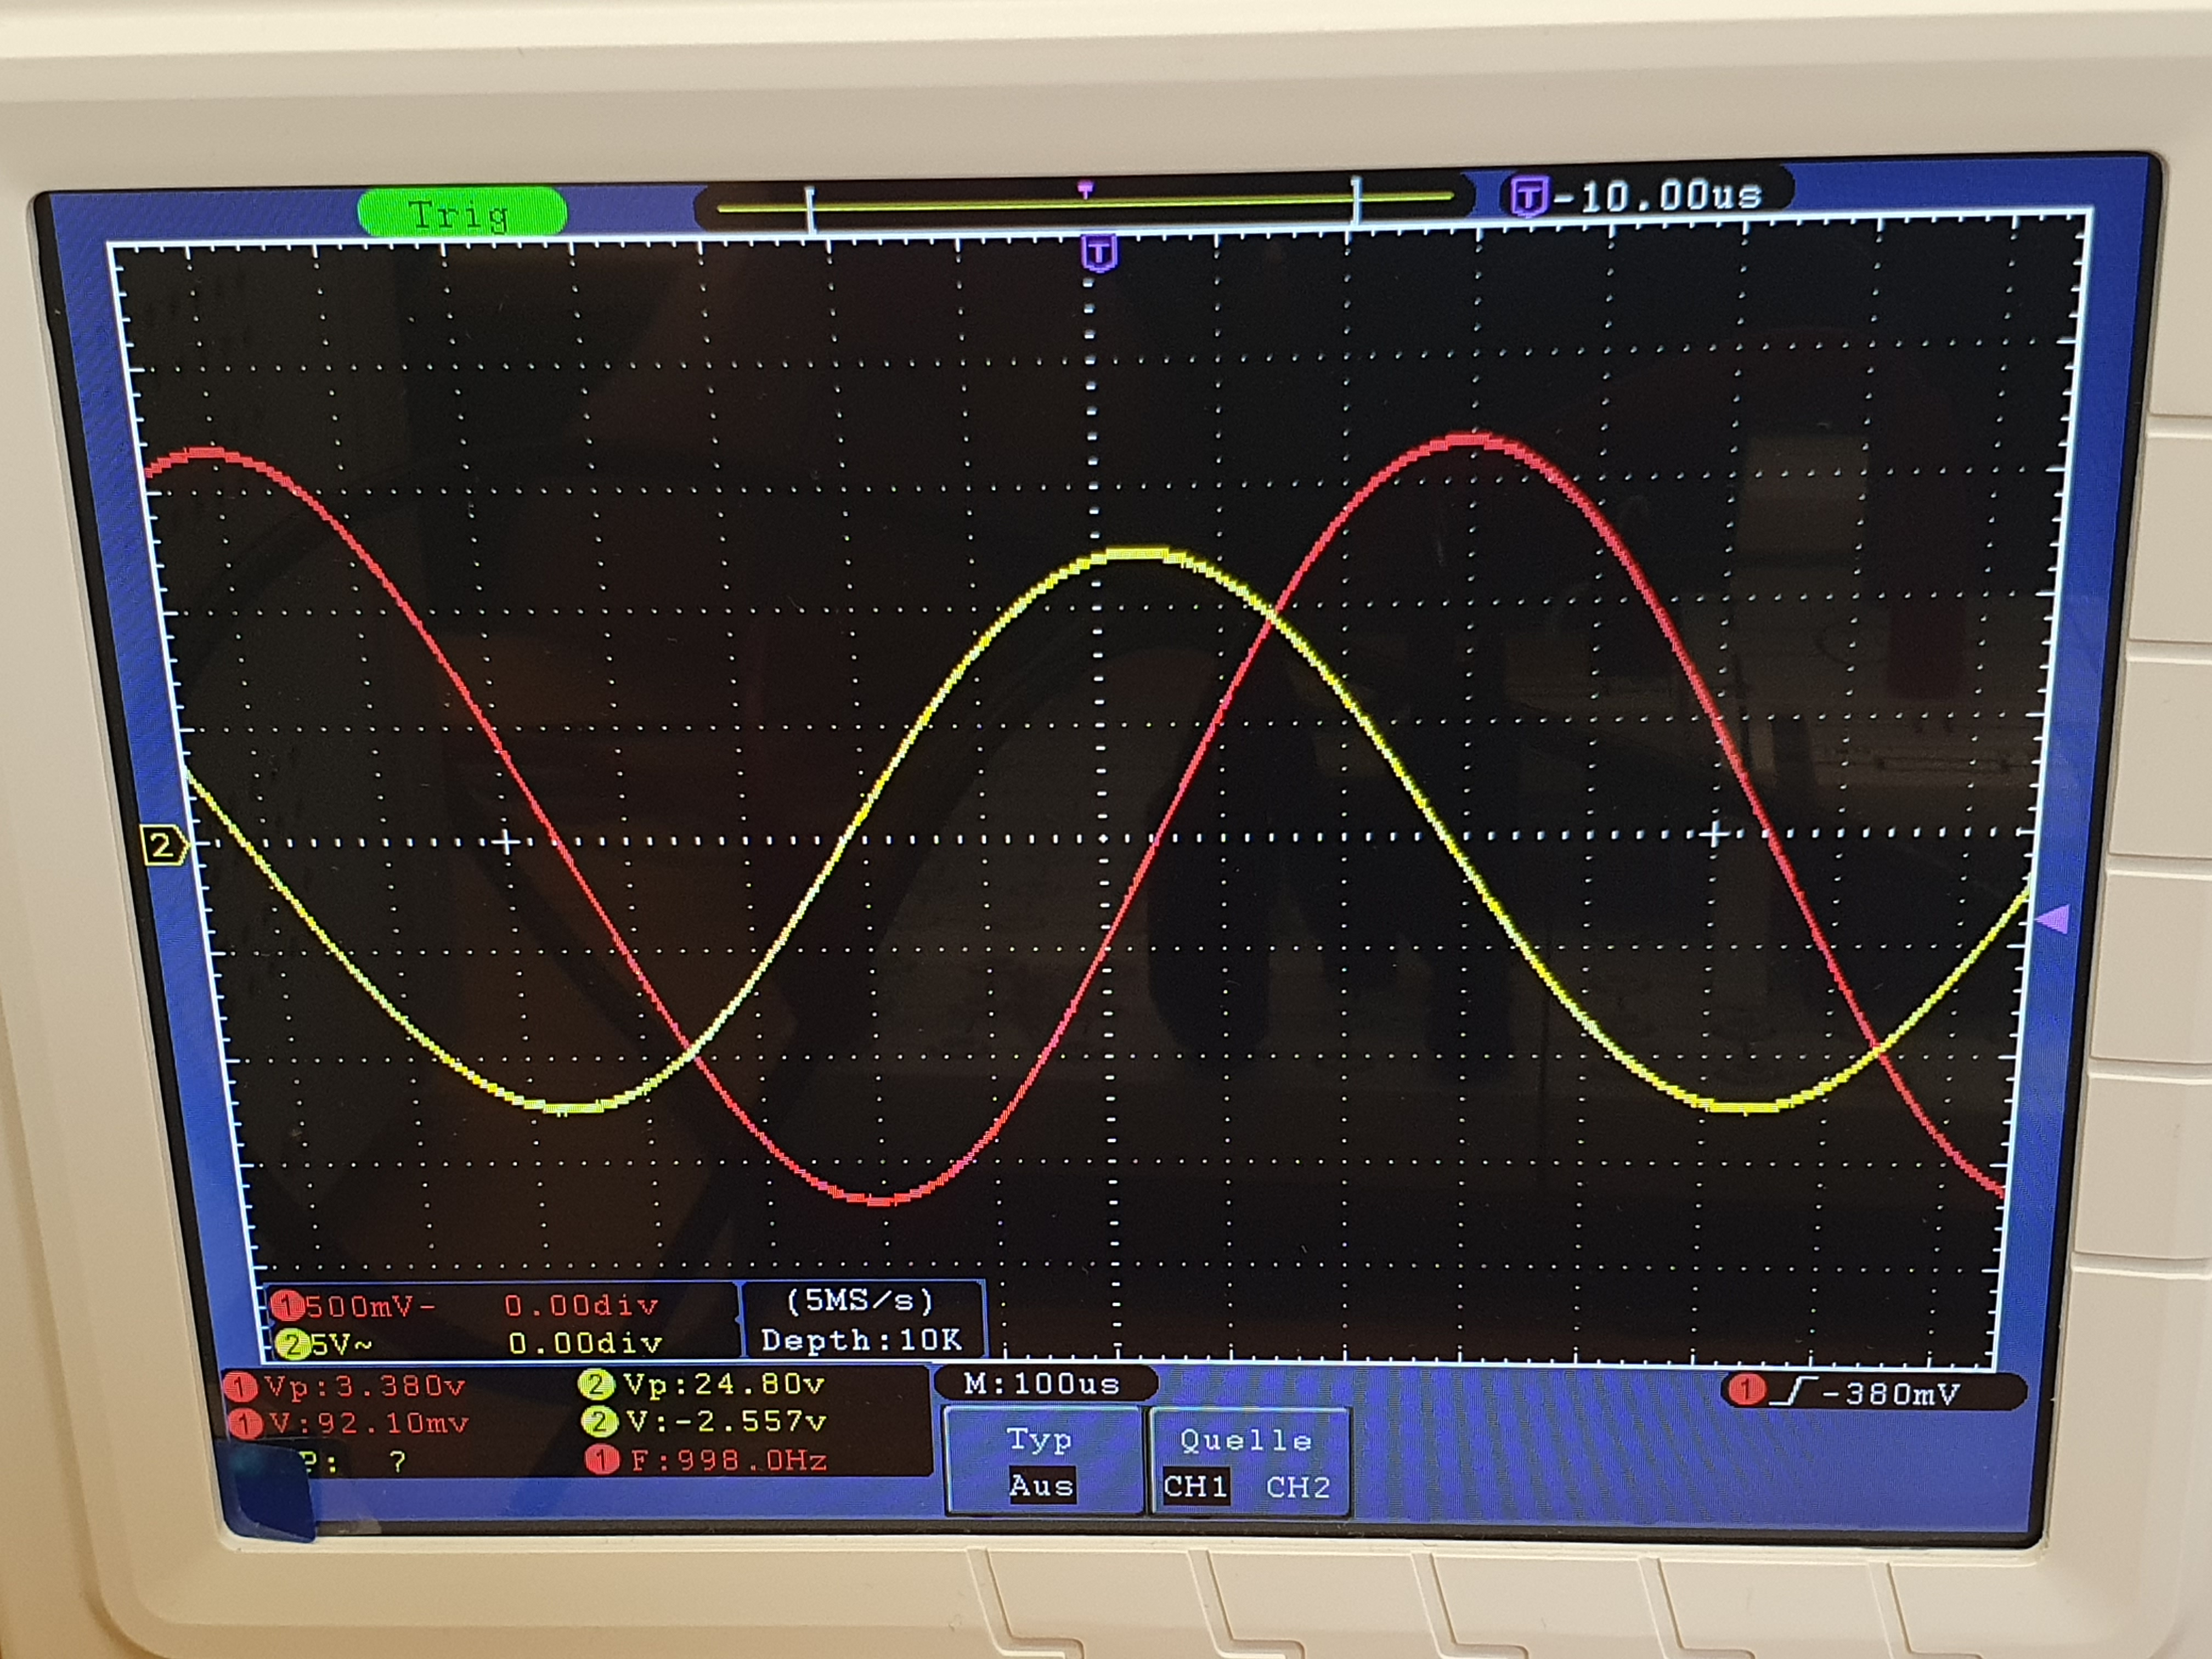
\includegraphics[width=0.4\linewidth]{nudes/messergebnisse/IntegriererSinusResultat.jpg}
    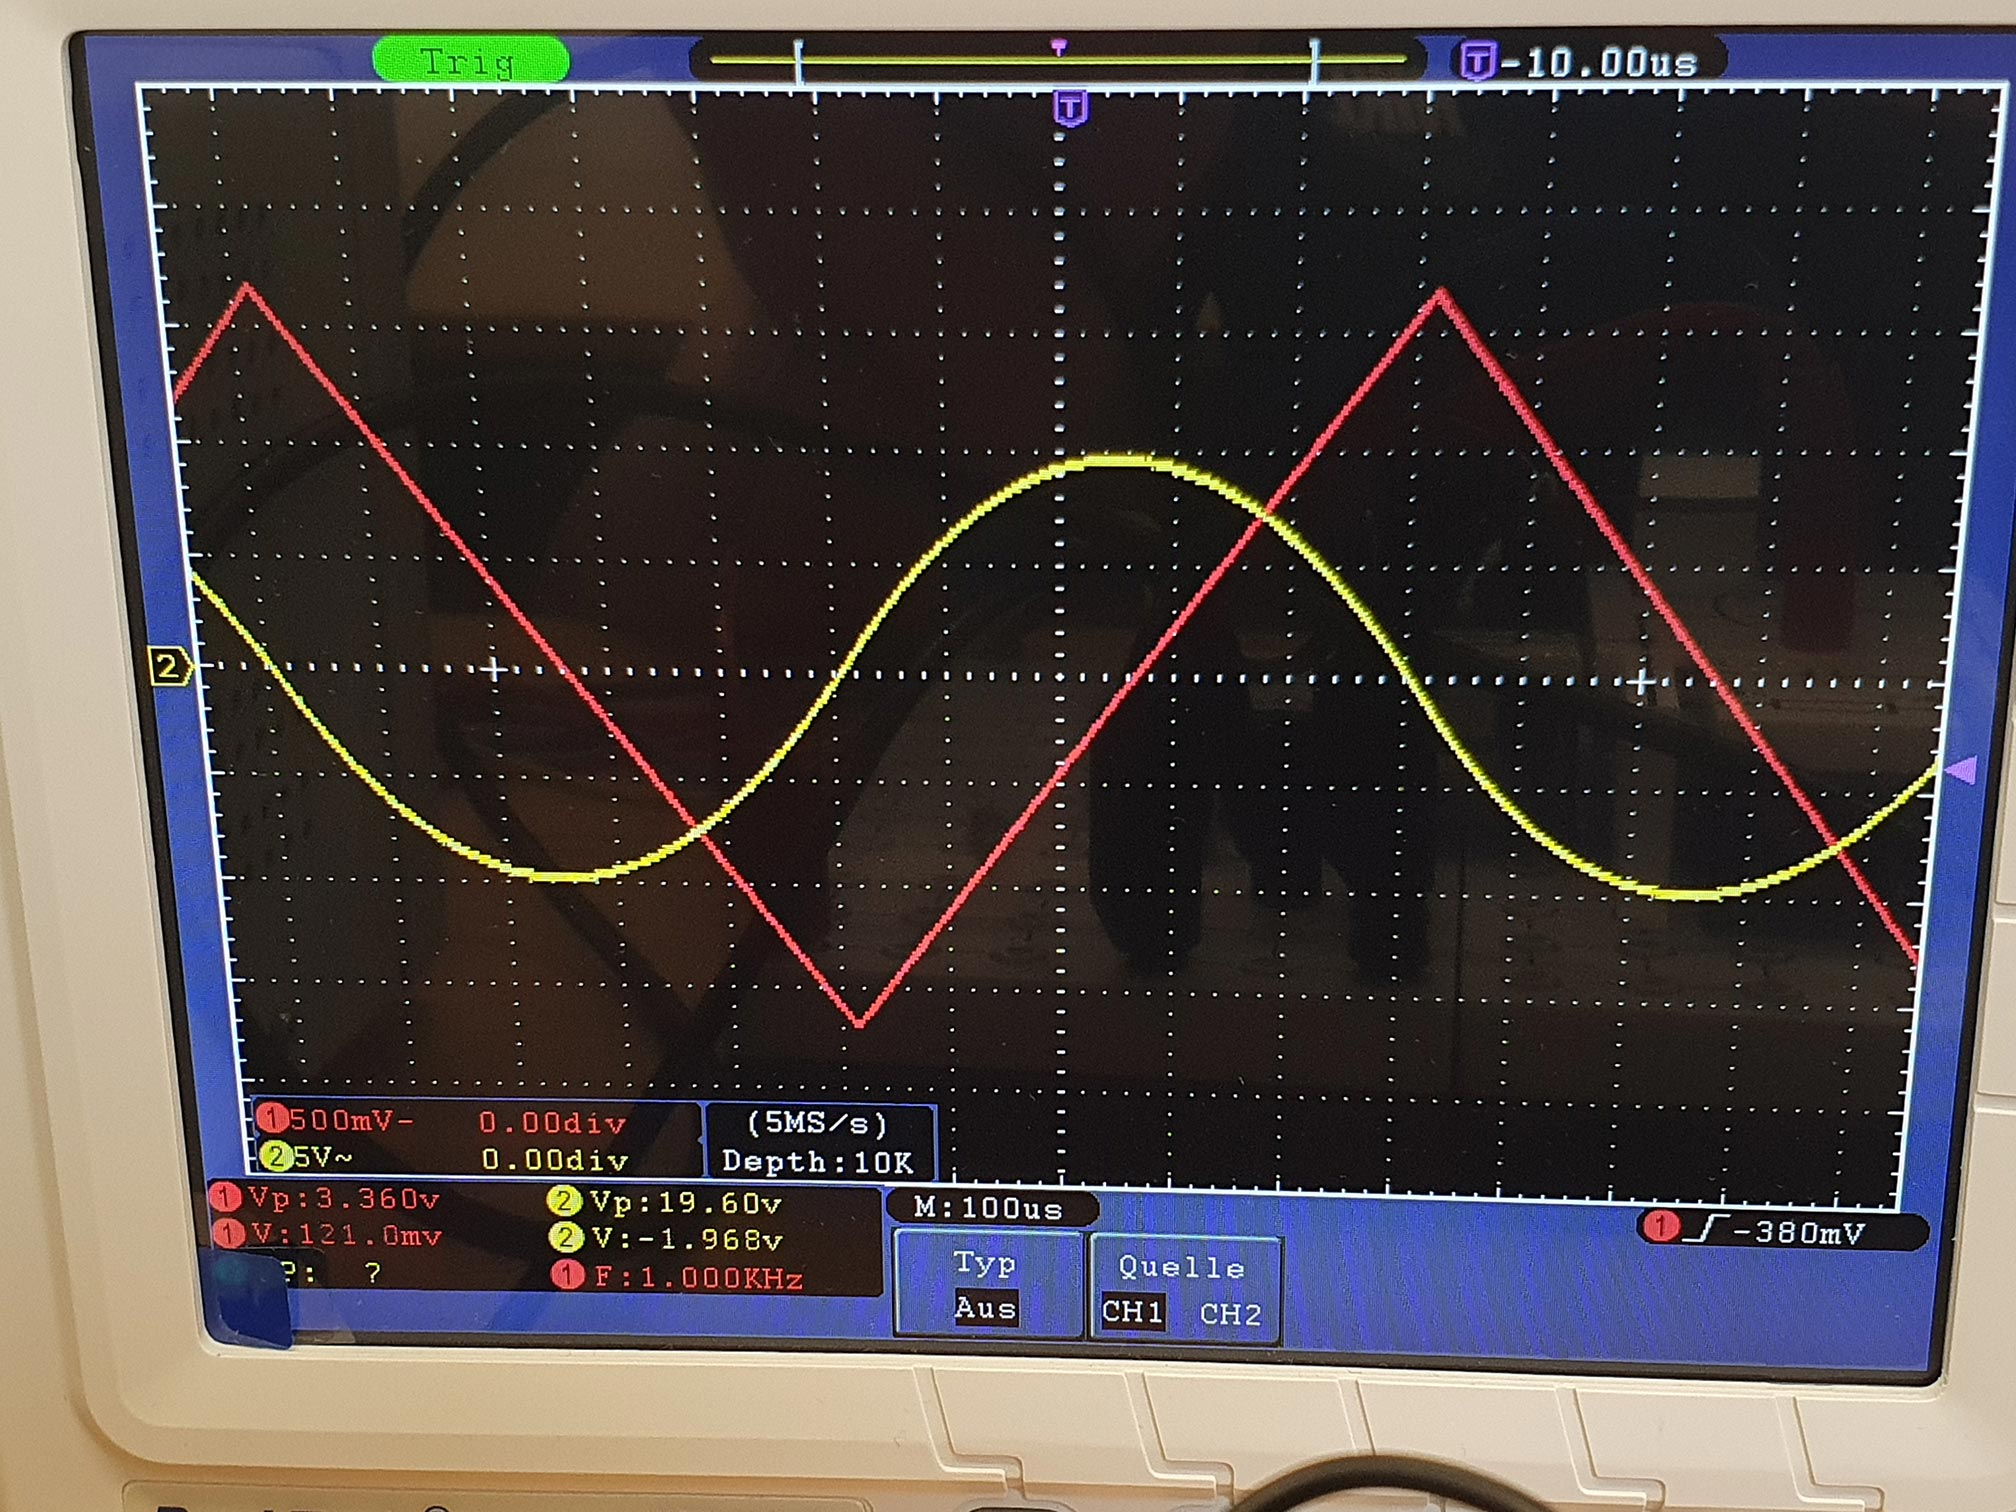
\includegraphics[width=0.4\linewidth]{nudes/messergebnisse/IntegriererDreieckResultat.jpg}
    \caption{Integrierer Sinus/Dreieck}
    \label{fig:IntegriererResultat3}
\end{figure}


\section{Auswertung und Unsicherheitsanalyse} %Nicht nur zahlen angeben ------------------------------

In der Auswertung werden zur erhöhten Genauigkeit durchgehend ungerundete Werte bis zu den Endergebnissen verwendet und nur zur Darstellung gerundet. \\
Zur Berechnung der Unsicherheiten wird, wenn nicht anders angegeben, die Größtunsicherheitsmethode verwendet.

\subsection{Komperatorschaltungen}

Die OPV-Schaltung dient als Komperator, wenn sie anzeigt, welche der beiden Eingangsspannungen größer ist. Ist die Spannung am invertierenden Eingang größer, so nähert sich die Ausgangsspannung der positiven Sättigungsspannung (in unserem Fall 15 V) an. 
Ist das eingehende Signal am nichtinvertierenden Eingang größer, so nähert sich die Ausgangsspannung der negativen Sättigungsspannung (in unserem Fall -15 V) an. \newline

\noindent
Da die laut Tabelle \ref{tab:Grundschaltung1Messungen} größere Spannung $U_{Ein2}$ an die nichtinvertierenden eingespeist wird, müssen für eine Komperatorwirkung genäherte Werte an -15 V am Ausgang gemessen werden. Dies trifft mit -13,15 $\pm$  V auch zu, was die Schaltung als funktionstüchtigen Komperator bestätigt. \newline

\noindent
Die Ausgangswerte der zweiten Komperatorschaltung werden am Oszilloskop wie in Abbildung \ref{fig:Grundschaltung2Ergebniss} ersichtlich als Rechteckspannung angezeigt. 
Eine Variation des Widerstandswertes am Potentiometer führt zu einer Vergrößerung bzw. Verkleinerung des positiven bzw. des negativen Spannungsanteils. Wird der Wert des Potentiometers stark verändert, so ergibt sich als Ausgangssignal ab einem gewissen Punkt eine horizontale Linie, was im Prinzip einer Gleichspannung entspricht. 


\subsection{Invertierender Verstärker}

Aus den Tabellen \ref{tab:IoVerstärkungenGemessen10} - \ref{tab:IoVerstärkungenGemessen100} ergeben sich mit Formel \ref{eq:InvertierenderVerstärkerVerstärkung} (und Formel \ref{eq:VerstärkungDezibel} die Verstärkung in dB) folgende Verstärkungen für die jeweiligen Widerstände $R_{2}$:

\begin{table}[H]
    \centering
    \caption{Invertierender OPV 10 k$\Omega$ Verstärkung Berechnung}
    \label{tab:IoVerstärkungenBerechnet10}
    \begin{tabular}{| l | l | l |}
        \hline
        Nr. & Verstärkung / & Verstärkung / dB \\
        \hline
        1 & -1.02 $\pm$ 0.03 & -0.2 $\pm$ 0.3 \\
        2 & -1.02 $\pm$ 0.03 & -0.2 $\pm$ 0.3 \\
        3 & -1.02 $\pm$ 0.03 & -0.2 $\pm$ 0.3 \\
        4 & -1.00 $\pm$ 0.05 &  0.0 $\pm$ 0.5 \\
        5 & -1.00 $\pm$ 0.05 &  0.0 $\pm$ 0.5 \\
        6 & -1.00 $\pm$ 0.05 &  0.0 $\pm$ 0.5 \\
        7 & -1.00 $\pm$ 0.05 &  0.0 $\pm$ 0.5 \\
        \hline
    \end{tabular}
\end{table}

\begin{table}[H]
    \centering
    \caption{Invertierender OPV 33 k$\Omega$ Verstärkung Berechnung}
    \label{tab:IoVerstärkungenBerechnet33}
    \begin{tabular}{| l | l | l |}
        \hline
        Nr. & Verstärkung / & Verstärkung / dB \\
        \hline
        1 & -3.31 $\pm$ 0.04 & -10.40 $\pm$ 0.11 \\
        2 & -3.30 $\pm$ 0.10 & -10.4 $\pm$ 0.3 \\
        3 & -3.34 $\pm$ 0.09 & -10.5 $\pm$ 0.3 \\
        4 & -3.10 $\pm$ 0.18 & -9.8 $\pm$ 0.6 \\
        5 & -3.3248 $\pm$ 0.09 & -10.4 $\pm$ 0.3 \\
        6 & -3.3247 $\pm$ 0.10 & -10.4 $\pm$ 0.3 \\
        7 & -3.3288 $\pm$ 0.04 & -10.45 $\pm$ 0.11 \\
        \hline
    \end{tabular}
\end{table}

\begin{table}[H]
    \centering
    \caption{Invertierender OPV 100 k$\Omega$ Verstärkung Berechnung}
    \label{tab:IoVerstärkungenBerechnet100}
    \begin{tabular}{| l | l | l |}
        \hline
        Nr. & Verstärkung / & Verstärkung / dB \\
        \hline
        1 & -8.98 $\pm$ 0.19 & 19.06 $\pm$ 0.19 \\
        2 & -10.2 $\pm$ 0.3 & 20.1 $\pm$ 0.3 \\
        3 & -10.1 $\pm$ 0.4 & 20.1 $\pm$ 0.4 \\
        4 & -10.4 $\pm$ 0.6 & 20.4 $\pm$ 0.6 \\
        5 & -10.2 $\pm$ 0.4 & 20.1398 $\pm$ 0.4 \\
        6 & -10.2 $\pm$ 0.3 & 20.1414 $\pm$ 0.3 \\
        7 & -8.65 $\pm$ 0.18 & 18.74 $\pm$ 0.19 \\
        \hline
    \end{tabular}
\end{table}

\noindent
Wie in den Tabellen ersichtlich ist, bestätigt sich die Beziehung für $U_{Ein}$ und $U_{Aus}$ aus Gleichung \ref{eq:InvertierenderVerstärkerVerstärkung}.
Die invertierende Verstärkerschaltung gibt ein invertiertes und je nach Widerstand $R_{2}$ verstärktes Signal aus. Somit ergibt sich eine Phasendifferenz von 180° zwischen Ein- und Ausgangssignal.


\subsection{Nicht invertierender Verstärker}

Wie in Abbildung \ref{fig:Nichtinvertierender10k10kOszibild} ersichtlich, haben $U_{Ein}$ und $U_{Aus}$ eine Phase von 0° zueinander, dass heißt sie schwingen gleichphasig.
Der Eingangswiderstand $R_{1}$ dient dazu, die Eingangsspannung klein zu halten, damit die Signalquelle nicht alzusehr belastet werden muss. Der Rückkopplungswiderstand $R_{2}$ bestimmt die Verstärkung des invertierenden OPVs. \newline

\noindent
Werden $R_{1}$ und $R_{2}$ nun unterschiedlich gewählt, so bleibt die Phasendifferenz zwar bei 0°, jedoch lassen sich unterschiedliche Verstärkungen feststellen. 
Mit den Werten aus Tabelle \ref{tab:NioVerstärkungenGemessen} kann mittels Formeln \ref{eq:NichtinvertierenderVerstärkerVerstärkung} und \ref{eq:VerstärkungDezibel} die Verstärkung berechnet werden. Da für diese lediglich das Verhältnis der beiden Signale benötigt wird, kann anstelle der tatsächlichen Spannungswerte auch die Amplitudenhöhe (in "Oszilloskop-Kästchen") verwendet werden.
Zu der Oszilloskopunsicherheit von $\pm$ 0.015 V wurde noch eine Ableseungenauigkeit von 0.2 Kästchen addiert.

\begin{table}[H]
    \centering
    \caption{NichtInvertierender OPV Verstärkungen Berechnungen}
    \label{tab:NioVerstärkungenBerechnet}
    \begin{tabular}{| l | l | l |}
        \hline
        Nr. & $\frac{Kaestchen}{Kaestchen}$ = V / & V / dB \\
        \hline
        1 & $\frac{1.0}{1.0}$ =  1.00 $\pm$ 0.43 & 0.0    $\pm$ 0.4 \\
        2 & $\frac{2.2}{1.5}$ =  1.5 $\pm$ 0.4 & 3.3 $\pm$ 0.3 \\
        3 & $\frac{3.7}{1.5}$ =  2.5 $\pm$ 0.5 & 7.84 $\pm$ 0.18 \\
        4 & $\frac{4.8}{1.5}$ =  3.2 $\pm$ 0.7 & 10.10 $\pm$ 0.20 \\
        5 & $\frac{4.4}{0.7}$ =  6.3 $\pm$ 1.2 & 15.97 $\pm$ 0.17 \\
        6 & $\frac{4.1}{0.4}$ = 10.3 $\pm$ 1.7 & 20.22 $\pm$ 0.15 \\
        \hline
    \end{tabular}
\end{table}

\noindent
Auch hier lässt sich der Zusammenhang \ref{eq:NichtinvertierenderVerstärkerVerstärkung} bestätigen.

\begin{figure}[H]
    \centering
    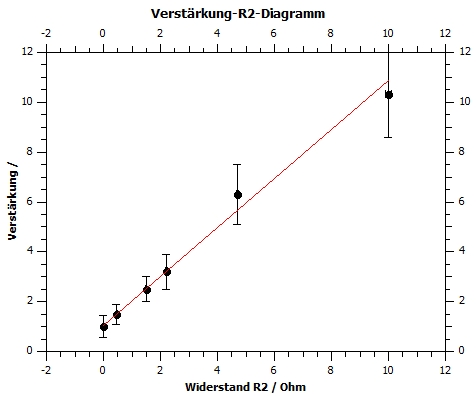
\includegraphics[width=0.5\linewidth]{nudes/NivVerstärkungR2Diagramm.jpg}
    \caption{Diagramm Verstärkung / Widerstand $R_{2}$ beim nichtinvertierenden Verstärker}
    \label{fig:Verstärkung/R2NIV}
\end{figure}


\subsection{Differenzierer}

Nun gilt es zu überprüfen, ob der Differenzierer tatsächlich das tut, was sein Name vermuten lässt - Differenzieren. Hierfür wird zunächst die Abbildung \ref{fig:Differenzierer0R1} untersucht.
Dabei stellt man fest, dass ohne einen Eingangswiderstand ein sehr ungenaues und zur Auswertung fast schon ungeeignetes Ergebniss geliefert wird. \newline

\noindent
Dieses Problem wurde jedoch mit einem Eingangswiderstand wie in Abbildung \ref{fig:Differenzierer1R1} gelöst.
Hier lässt sich nun ein schöneres und brauchbares Ergebniss beobachten. Da die Ableitung die Steigung der Eingangsfunktion darstellt, lässt sich das Ergebnis so auch grob kontrollieren. 
Bei der Rechteckspannung ist die Steigung an den Punkten, an denen sich das Signal umkehrt sehr hoch bzw. sehr niedrig und an den restlichen Stellen 0. Dies ist in Abbildung \ref{fig:Differenzierer1R1} sehr gut erkennbar und bestätigt die Funktion der Schaltung als Differenzierer. \newline

\noindent
Das Gleiche lässt sich auch über Abbildungen \ref{fig:Differenzierer1R1Sinus/Dreieck} sagen. Die Ableitung des Sinus ist der Cosinus, der auch als Ausgangssignal im eben genannten Bild abgebildet ist.
Bei der Dreiecksspannung resultiert ein Rechteckssignal, welches wiederum die abwechselnd positive- und negative Steigung der Dreiecke darstellt. 



\subsection{Integrierer}

Das große Finale des Versuches war am Ende noch der Integrierer, welcher in Theorie das Gegenstück zum Differenzierer darstellen und Eingangssignale integrieren sollte. 
Wie in Abbildung \ref{fig:IntegriererResultat1} erkennbar, wird das eingespeiste Rechteckssignal nun zur Dreiecksspannung, also genau die umgekehrte Funktion des Differenzierer. Aus den konstanten Signalen des Eingangs werden nun Funktionen erster Ordnung am Ausgang. \newline

\noindent
Der Widerstand R, welcher paralell zum Kondensator geschaltet wird, stellt dabei die Stabilität der Schaltung sicher und verhindert überbetonte Frequenzen. Wird der Kondensator nun auf 2.2 nF verringert, so erhält man ein Oszilloskopbild laut Abbildung \ref{fig:IntegriererResultat2}.
Da durch die kleinere Kapazität die Zeitkonstante (RC) kleiner wird, reagiert die Schaltung auf Veränderungen am Eingang schneller. Der Lade- und Entladevorgang ist in eben genannter Abbildung \ref{fig:IntegriererResultat2} außerdem an den Ausgangssignalen deutlicher zu erkennen. \newline

\noindent
Ein Blick auf Abbildungen \ref{fig:IntegriererResultat3} zeigt selbiges Prinzip für Sinus- und Dreiecksspannungen. Der integrierte Sinus ergibt als Ausgangssignal einen Cosinus, aus der Dreiecksspannung (Funktionen ersten Grades) wird eine Welle aus Parabeln (Funktionen zweiten Grades).
Diese Resultate spiegeln sich außerdem mit erwarteten Werten laut Gleichung \ref{eq:IntegriererAusgang} wieder. Die Ausgangsfunktion bildet also die Stammfunktion des Eingangssignales.




\section{Diskussion} %diskussion der Unsicherheiten und Ergebnisse und evtl. verlgeich mit Literatur ------------------------------

\subsection{Komperatorschaltungen}



\subsection{Invertierender Verstärker}



\subsection{Nichtinvertierender Verstärker}



\subsection{Differenzierer}



\subsection{Integrierer}




\section{Zusammenfassung} %klare, übersichtliche vollständige beantwortung der Aufgabenstellung ------------------------------

\subsection{Komperatorschaltungen}

\begin{table}[H]
    \centering
    \caption{Grundschaltung1 Messungen}
    \label{tab:Grundschaltung1MessungenAW}
    \begin{tabular}{| l | l | l | l |}
        \hline
        Nr. & $U_{Ein1}$ / V & $U_{Ein2}$ $\pm$ 0.01 / V & $U_{Aus1}$ $\pm$ 0.16 / V \\
        \hline
        1 & -0.0461 $\pm$ 0.0007 & -0.79 & -13.15 \\
        2 & -0.0833 $\pm$ 0.0010 & -0.79 & -13.15 \\
        3 & -0.0612 $\pm$ 0.0008 & -0.79 & -13.15 \\
        4 & -0.1069 $\pm$ 0.0013 & -0.79 & -13.15 \\
        5 & -0.0890 $\pm$ 0.0011 & -0.79 & -13.15 \\
        \hline
    \end{tabular}
\end{table}

\begin{figure}[H]
    \centering
    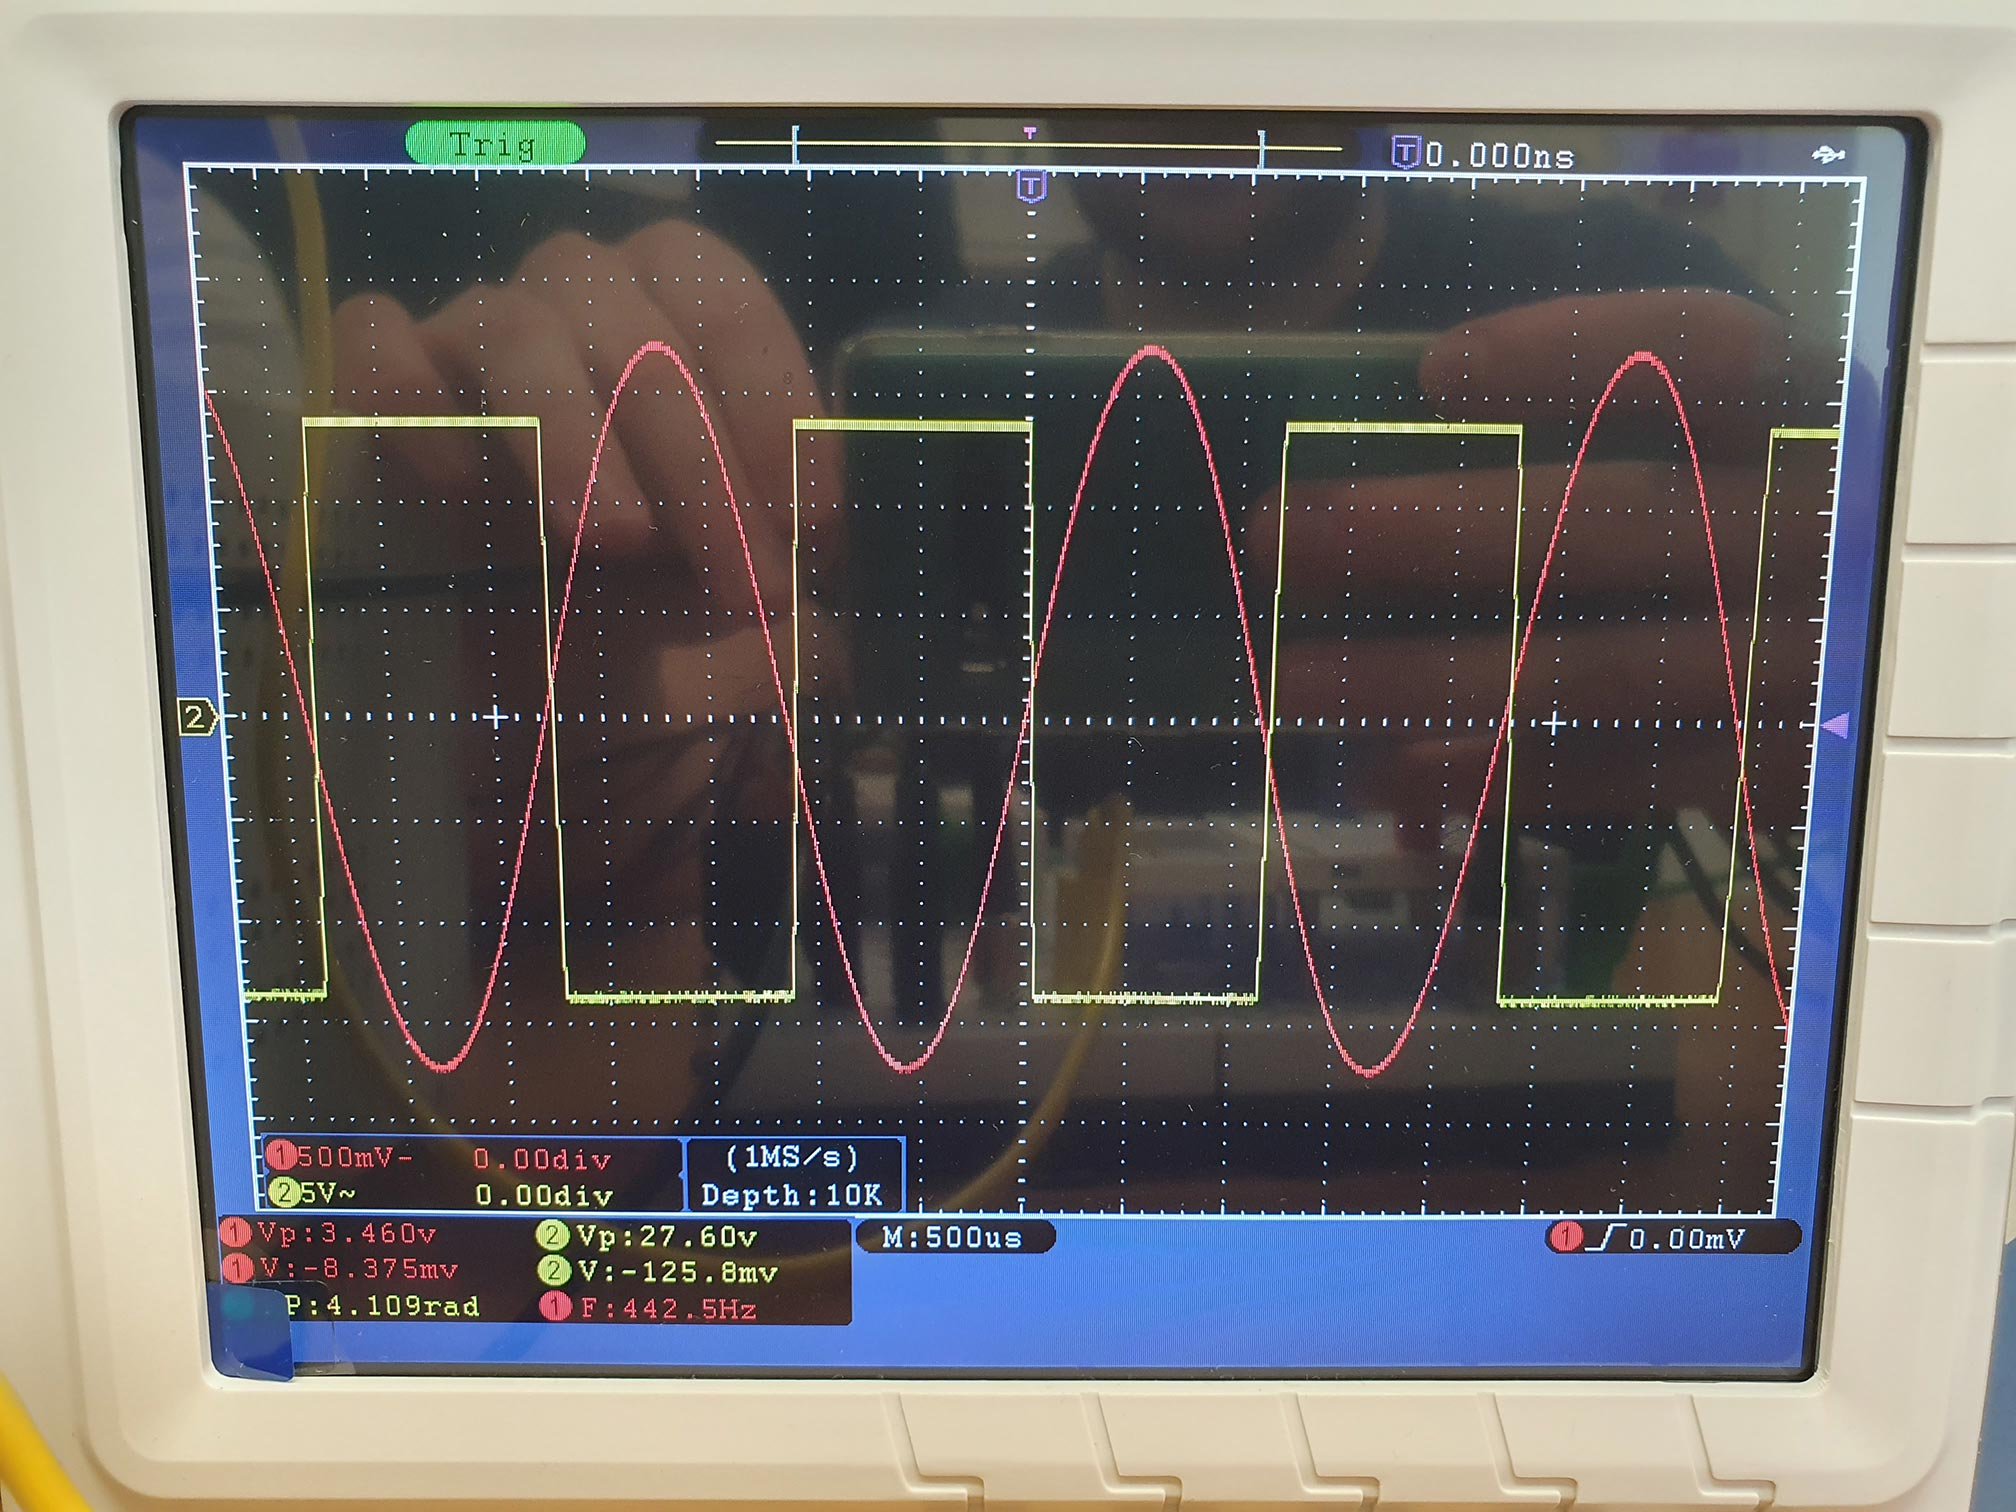
\includegraphics[width=0.4\linewidth]{nudes/messergebnisse/Grundschaltung2OsziErgebnis.jpg}
    \caption{Oszilloskopbild der zweiten Komperatorschaltung}
    \label{fig:Grundschaltung2ErgebnissAW}
\end{figure}

\begin{figure}[H]
    \centering
    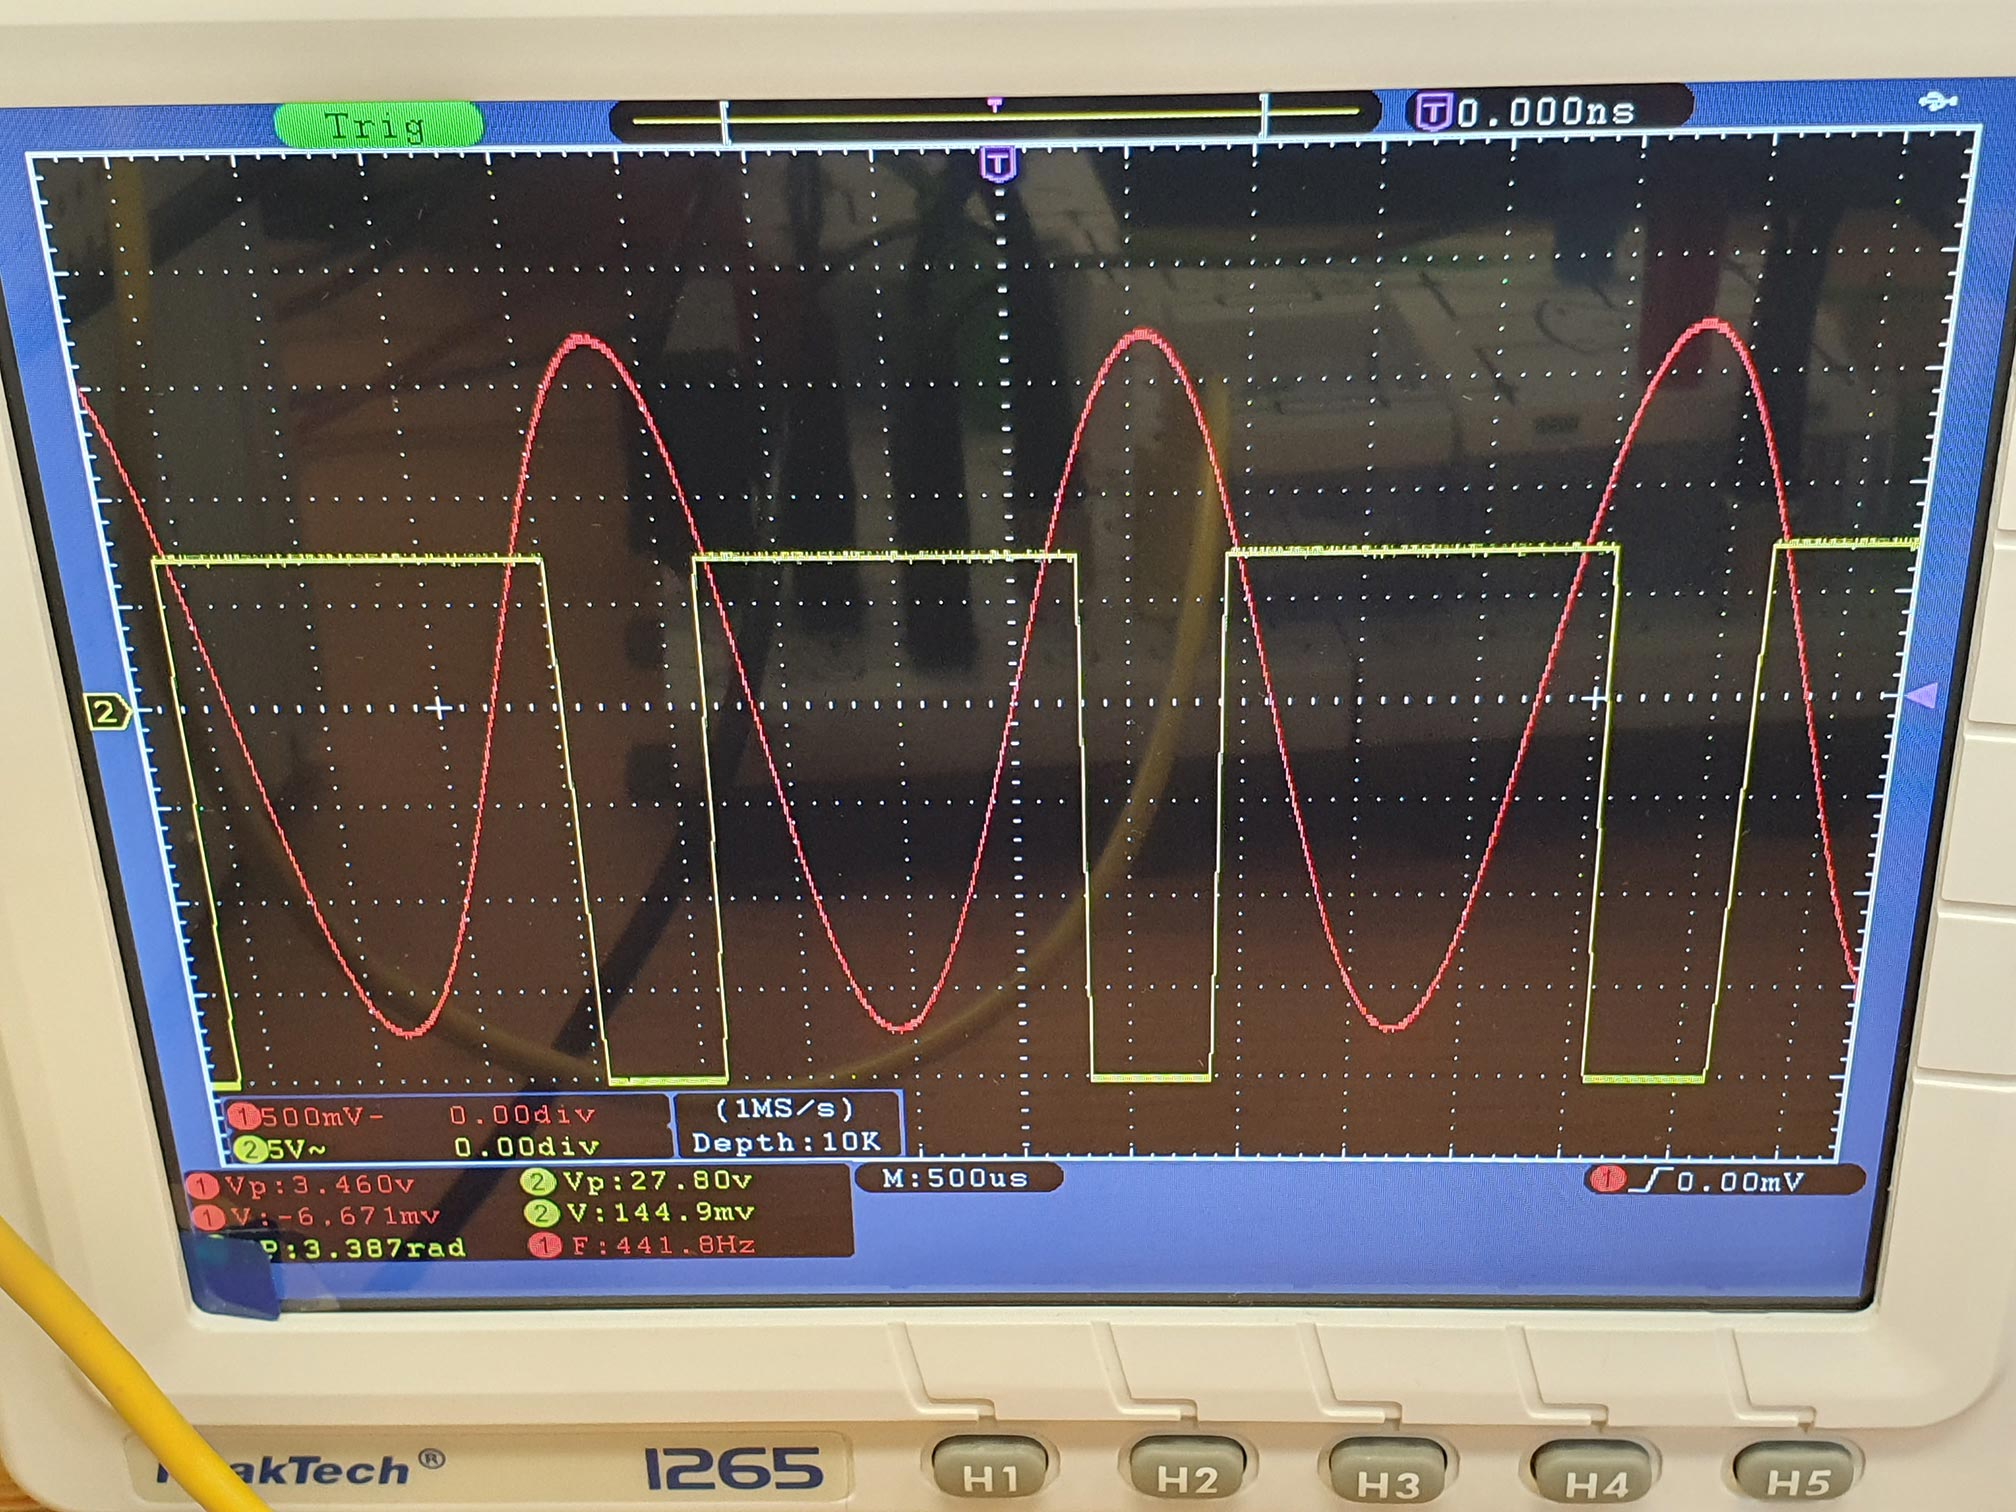
\includegraphics[width=0.4\linewidth]{nudes/messergebnisse/Grundschaltung2OsziErgebnislinks.jpg}
    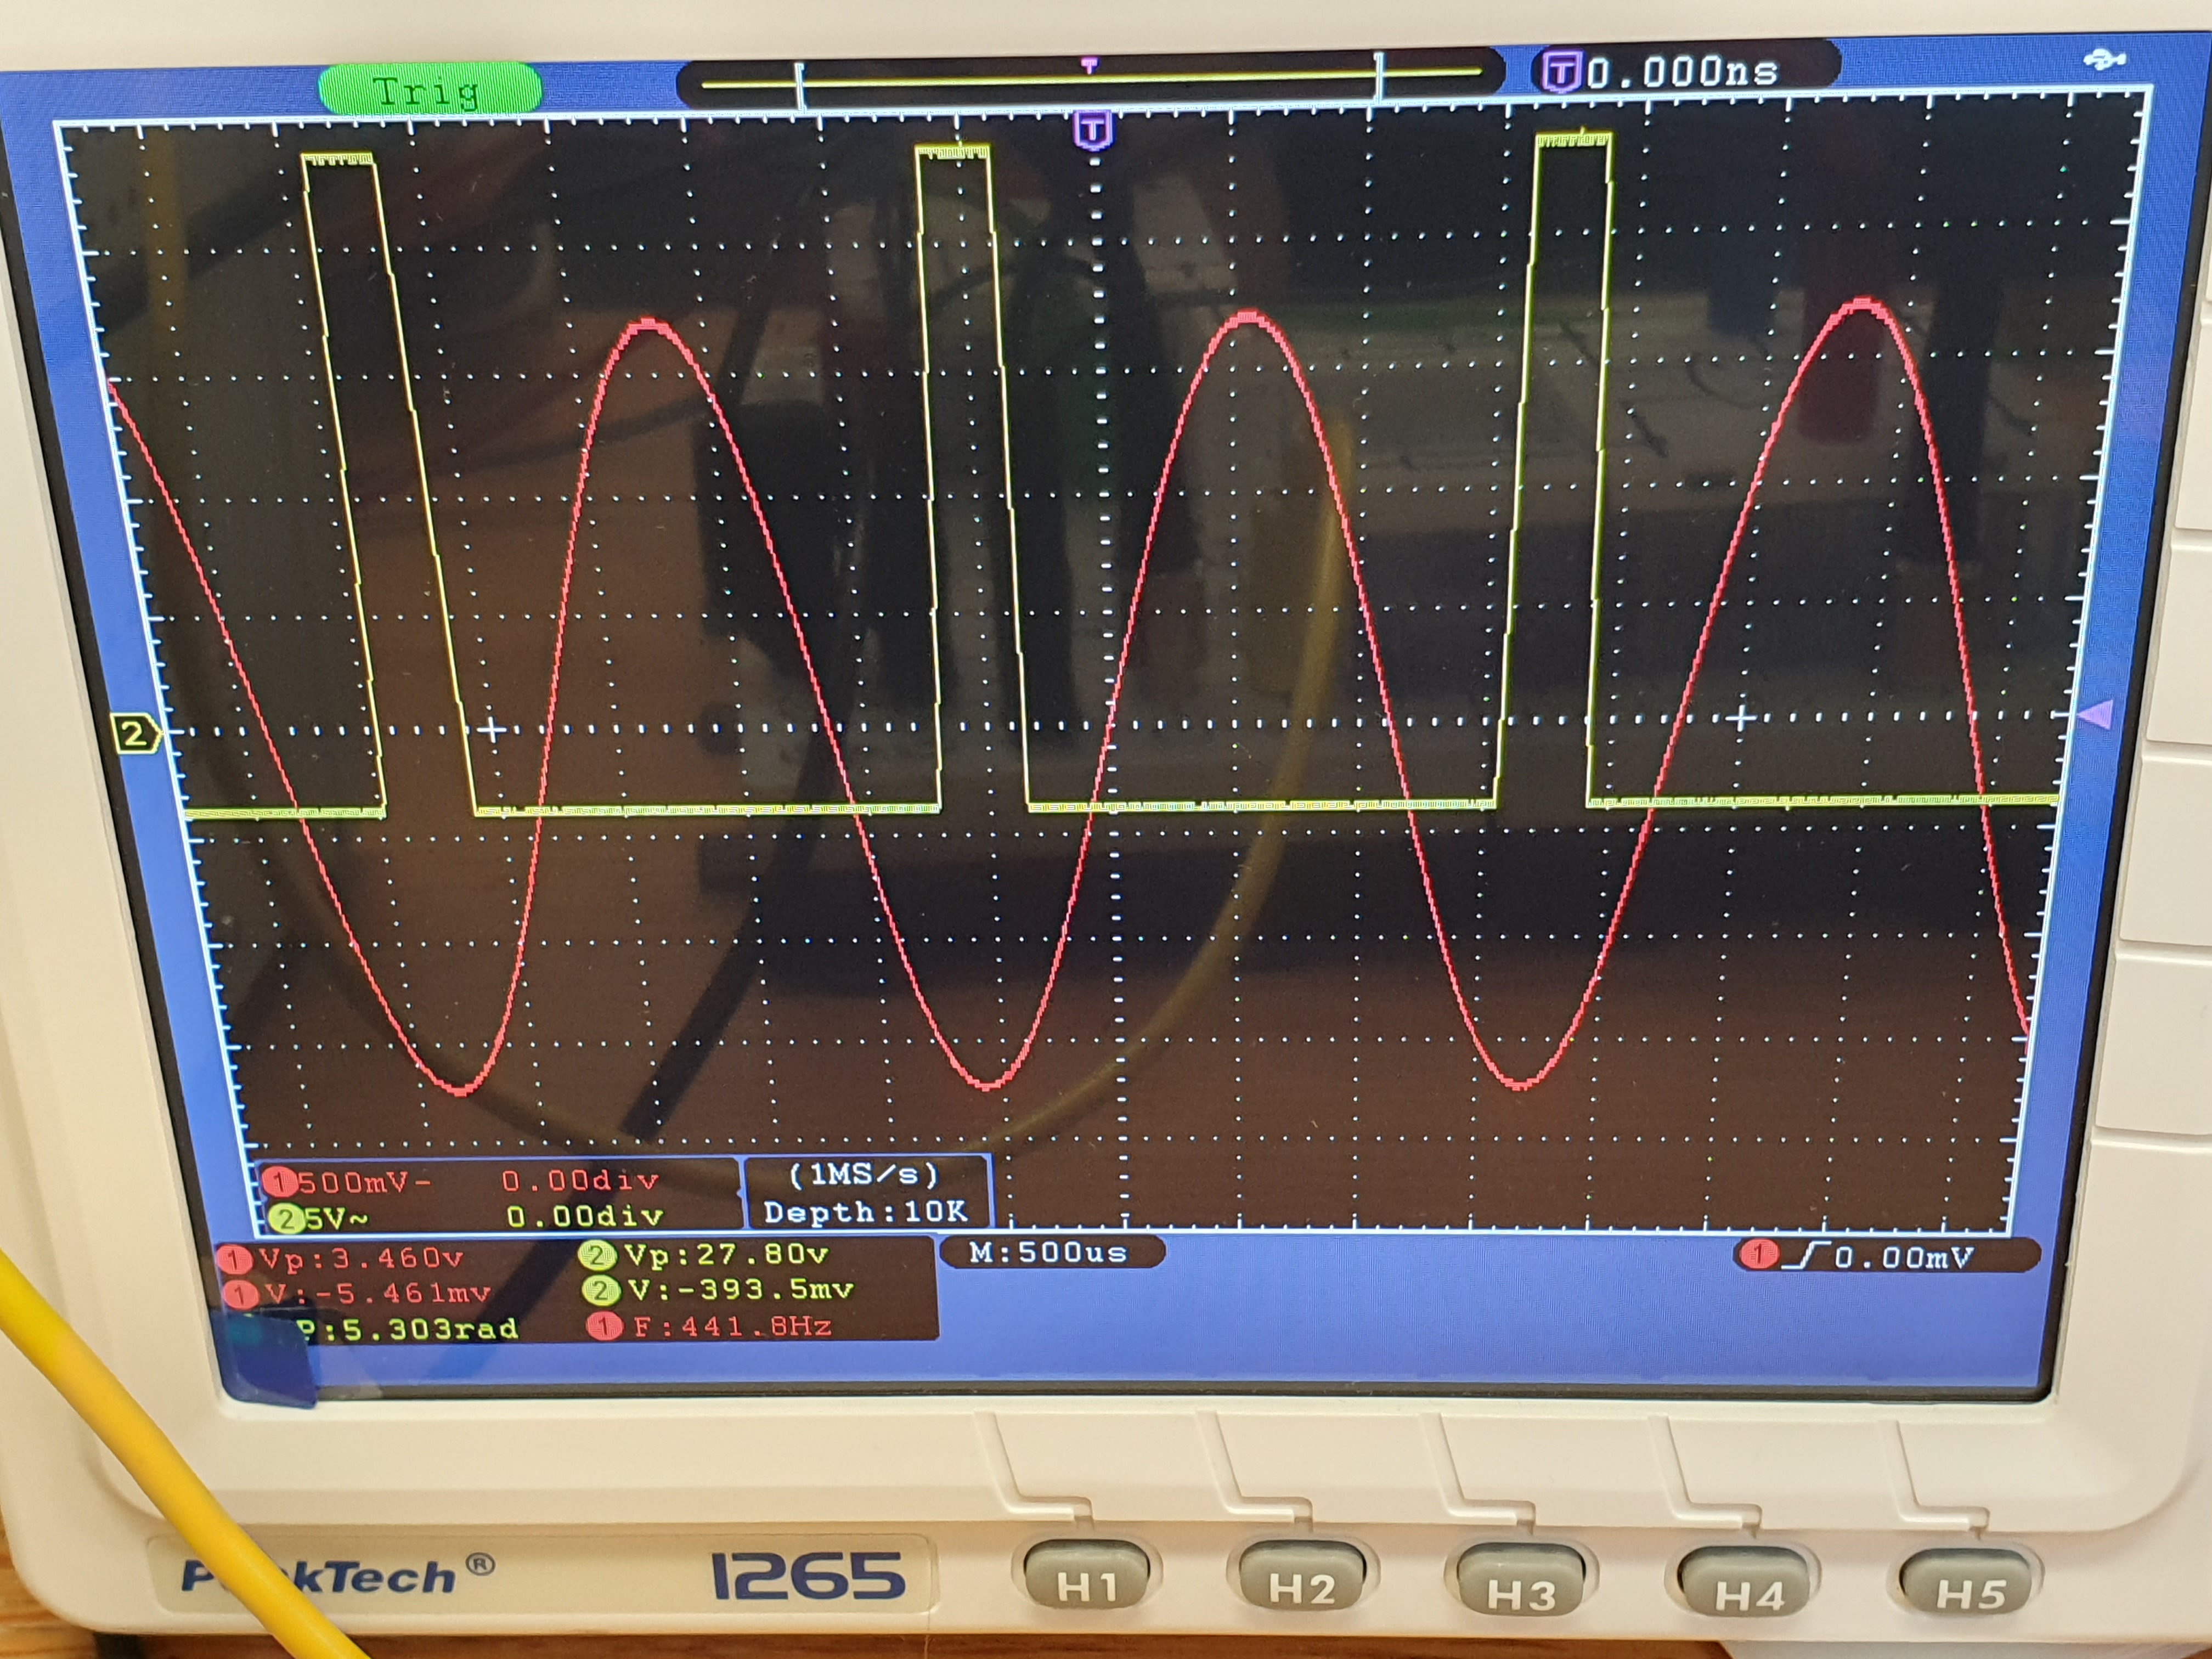
\includegraphics[width=0.4\linewidth]{nudes/messergebnisse/Grundschaltung2OsziErgebnisrechts.jpg}
    \caption{Oszilloskopbild der zweiten Komperatorschaltung mit größer/kleiner gestellten Widerstand}
    \label{fig:Grundschaltung2ErgebnissPotiAW}
\end{figure}


\subsection{Invertierender Verstärker}

\begin{table}[H]
    \centering
    \caption{Invertierender OPV 10 k$\Omega$ Verstärkung Berechnung}
    \label{tab:IoVerstärkungenBerechnet10AW}
    \begin{tabular}{| l | l | l |}
        \hline
        Nr. & Verstärkung / & Verstärkung / dB \\
        \hline
        1 & -1.02 $\pm$ 0.03 & -0.2 $\pm$ 0.3 \\
        2 & -1.02 $\pm$ 0.03 & -0.2 $\pm$ 0.3 \\
        3 & -1.02 $\pm$ 0.03 & -0.2 $\pm$ 0.3 \\
        4 & -1.00 $\pm$ 0.05 &  0.0 $\pm$ 0.5 \\
        5 & -1.00 $\pm$ 0.05 &  0.0 $\pm$ 0.5 \\
        6 & -1.00 $\pm$ 0.05 &  0.0 $\pm$ 0.5 \\
        7 & -1.00 $\pm$ 0.05 &  0.0 $\pm$ 0.5 \\
        \hline
    \end{tabular}
\end{table}

\begin{table}[H]
    \centering
    \caption{Invertierender OPV 33 k$\Omega$ Verstärkung Berechnung}
    \label{tab:IoVerstärkungenBerechnet33AW}
    \begin{tabular}{| l | l | l |}
        \hline
        Nr. & Verstärkung / & Verstärkung / dB \\
        \hline
        1 & -3.31 $\pm$ 0.04 & -10.40 $\pm$ 0.11 \\
        2 & -3.30 $\pm$ 0.10 & -10.4 $\pm$ 0.3 \\
        3 & -3.34 $\pm$ 0.09 & -10.5 $\pm$ 0.3 \\
        4 & -3.10 $\pm$ 0.18 & -9.8 $\pm$ 0.6 \\
        5 & -3.3248 $\pm$ 0.09 & -10.4 $\pm$ 0.3 \\
        6 & -3.3247 $\pm$ 0.10 & -10.4 $\pm$ 0.3 \\
        7 & -3.3288 $\pm$ 0.04 & -10.45 $\pm$ 0.11 \\
        \hline
    \end{tabular}
\end{table}

\begin{table}[H]
    \centering
    \caption{Invertierender OPV 100 k$\Omega$ Verstärkung Berechnung}
    \label{tab:IoVerstärkungenBerechnet100AW}
    \begin{tabular}{| l | l | l |}
        \hline
        Nr. & Verstärkung / & Verstärkung / dB \\
        \hline
        1 & -8.98 $\pm$ 0.19 & 19.06 $\pm$ 0.19 \\
        2 & -10.2 $\pm$ 0.3 & 20.1 $\pm$ 0.3 \\
        3 & -10.1 $\pm$ 0.4 & 20.1 $\pm$ 0.4 \\
        4 & -10.4 $\pm$ 0.6 & 20.4 $\pm$ 0.6 \\
        5 & -10.2 $\pm$ 0.4 & 20.1398 $\pm$ 0.4 \\
        6 & -10.2 $\pm$ 0.3 & 20.1414 $\pm$ 0.3 \\
        7 & -8.65 $\pm$ 0.18 & 18.74 $\pm$ 0.19 \\
        \hline
    \end{tabular}
\end{table}

\subsection{Nichtinvertierender Verstärker}

\begin{table}[H]
    \centering
    \caption{Nichtinvertierender OPV Verstärkungen Berechnungen}
    \label{tab:NioVerstärkungenBerechnetAW}
    \begin{tabular}{| l | l | l |}
        \hline
        Nr. & $\frac{Kaestchen}{Kaestchen}$ = V / & V / dB \\
        \hline
        1 & $\frac{1.0}{1.0}$ =  1.00 $\pm$ 0.43 & 0.0    $\pm$ 0.4 \\
        2 & $\frac{2.2}{1.5}$ =  1.5 $\pm$ 0.4 & 3.3 $\pm$ 0.3 \\
        3 & $\frac{3.7}{1.5}$ =  2.5 $\pm$ 0.5 & 7.84 $\pm$ 0.18 \\
        4 & $\frac{4.8}{1.5}$ =  3.2 $\pm$ 0.7 & 10.10 $\pm$ 0.20 \\
        5 & $\frac{4.4}{0.7}$ =  6.3 $\pm$ 1.2 & 15.97 $\pm$ 0.17 \\
        6 & $\frac{4.1}{0.4}$ = 10.3 $\pm$ 1.7 & 20.22 $\pm$ 0.15 \\
        \hline
    \end{tabular}
\end{table}

\noindent
Auch hier lässt sich der Zusammenhang \ref{eq:NichtinvertierenderVerstärkerVerstärkung} bestätigen.

\begin{figure}[H]
    \centering
    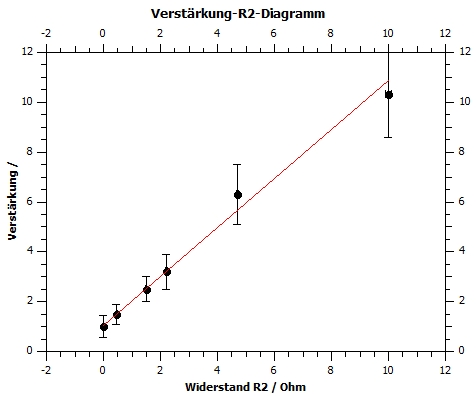
\includegraphics[width=0.5\linewidth]{nudes/NivVerstärkungR2Diagramm.jpg}
    \caption{Diagramm Verstärkung / Widerstand $R_{2}$ beim nichtinvertierenden Verstärker}
    \label{fig:Verstärkung/R2NIVAW}
\end{figure}

\subsection{Differenzierer}

\begin{figure}[H]
    \centering
    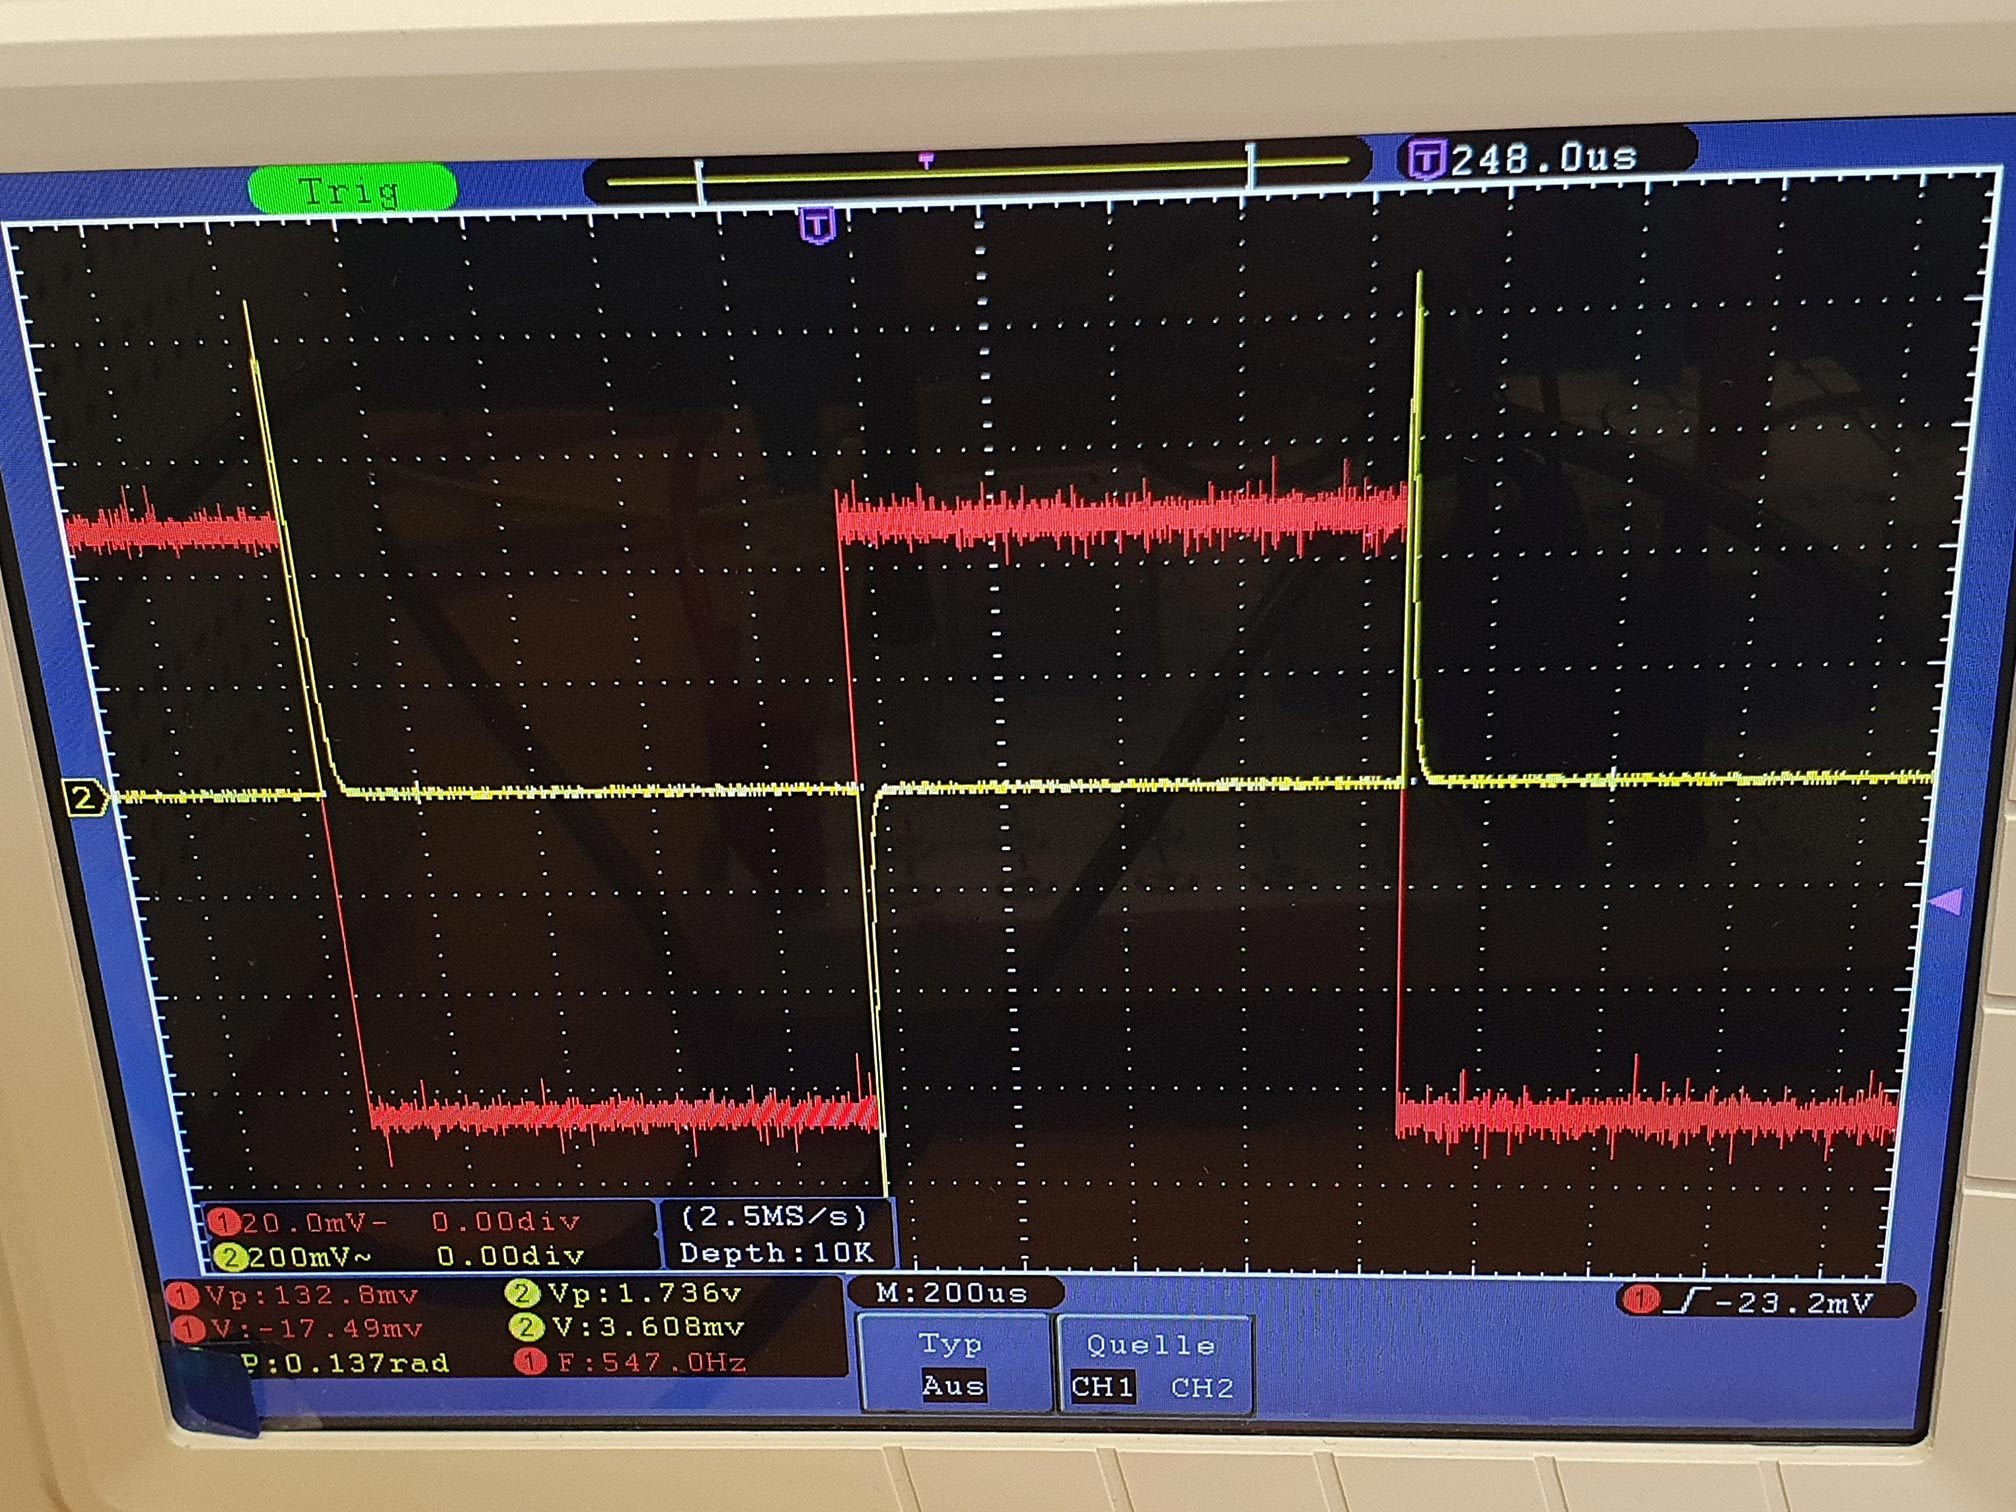
\includegraphics[width=0.4\linewidth]{nudes/messergebnisse/DifferenziererMitEingangsR.jpg}
    \caption{Differenzierer mit Eingangswiderstand 1 k$\Omega$}
    \label{fig:Differenzierer1R1AW}
\end{figure}

\begin{figure}[H]
    \centering
    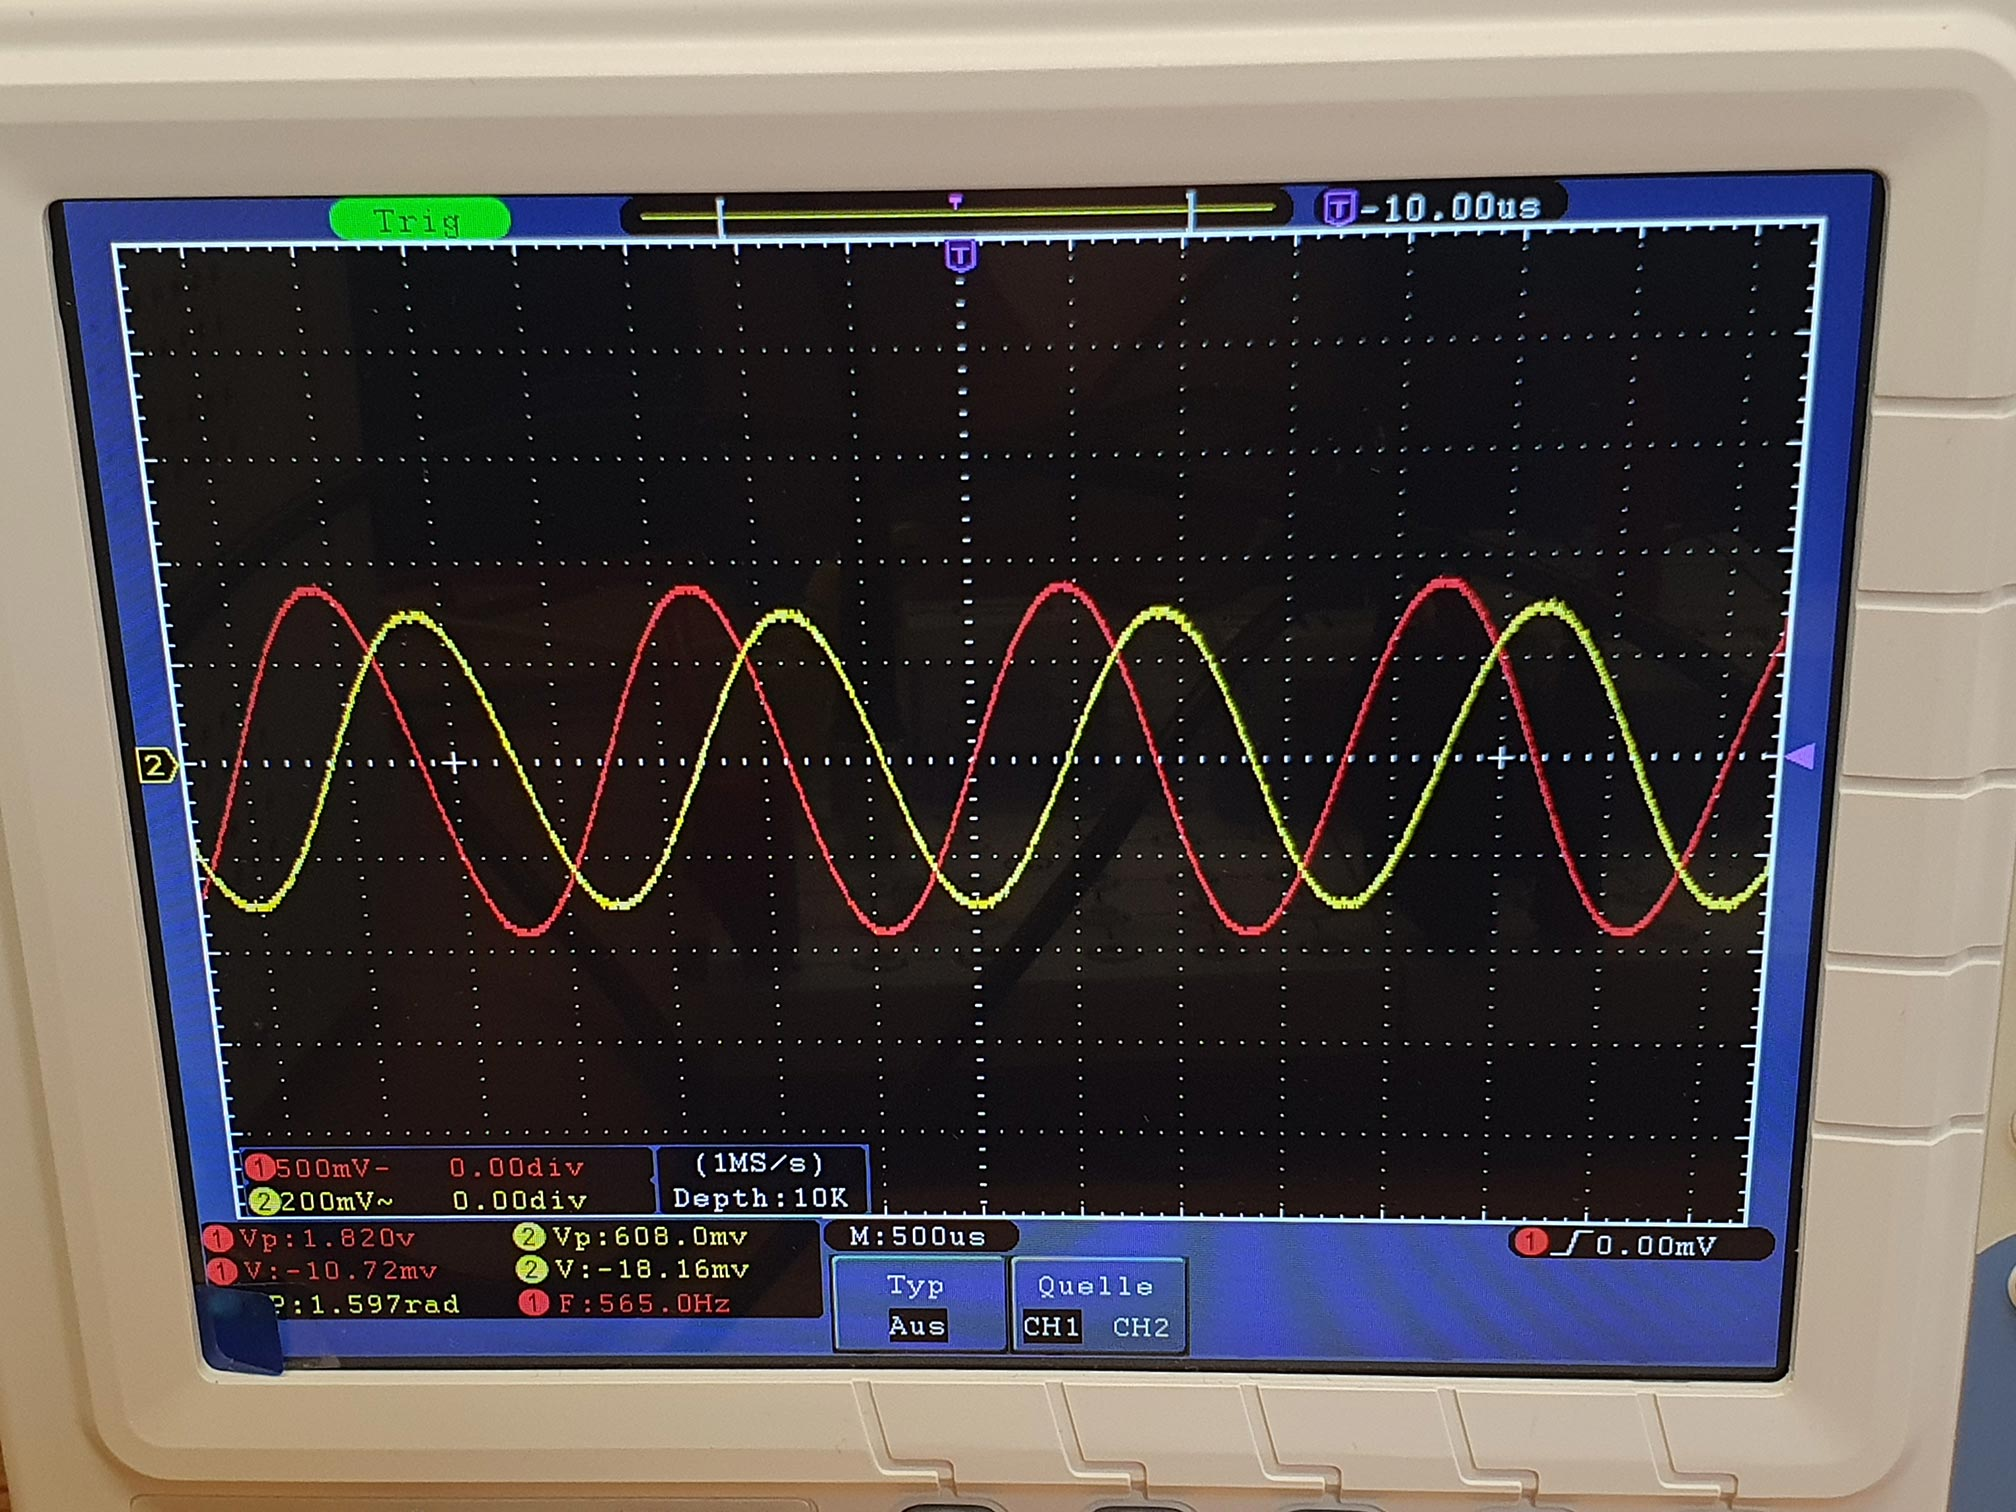
\includegraphics[width=0.4\linewidth]{nudes/messergebnisse/DifferenziererSinus.jpg}
    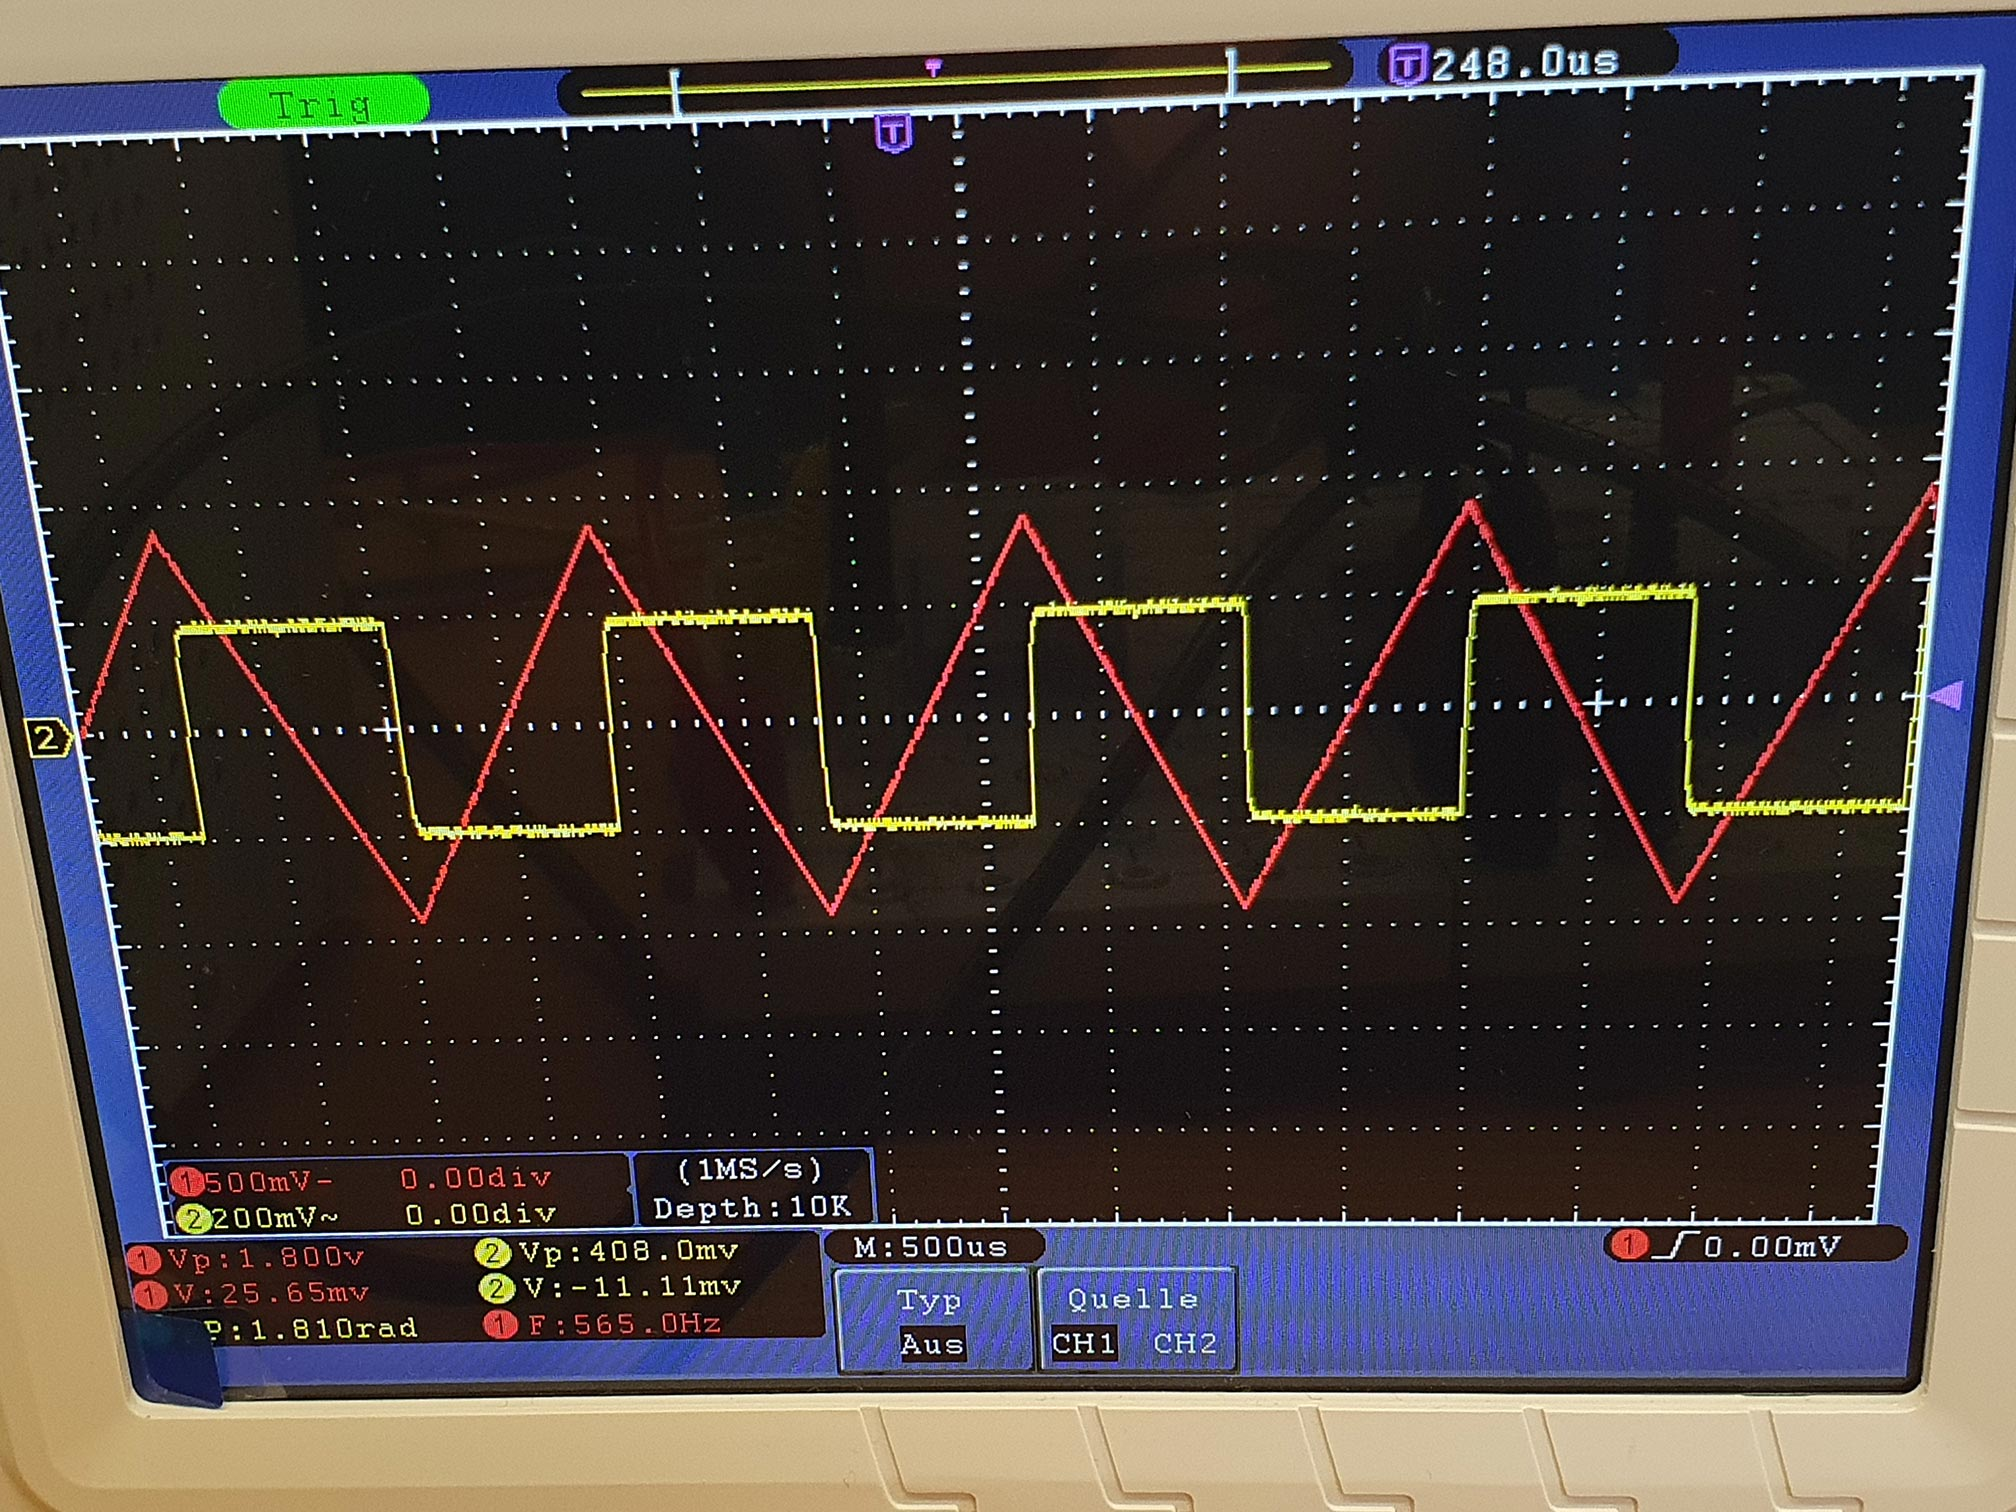
\includegraphics[width=0.4\linewidth]{nudes/messergebnisse/DifferenziererDreieck.jpg}
    \caption{Differenzierer mit Eingangswiderstand 1 k$\Omega$ Sinus/Dreieck}
    \label{fig:Differenzierer1R1Sinus/DreieckAW}
\end{figure}

\subsection{Integrierer}

\begin{figure}[H]
    \centering
    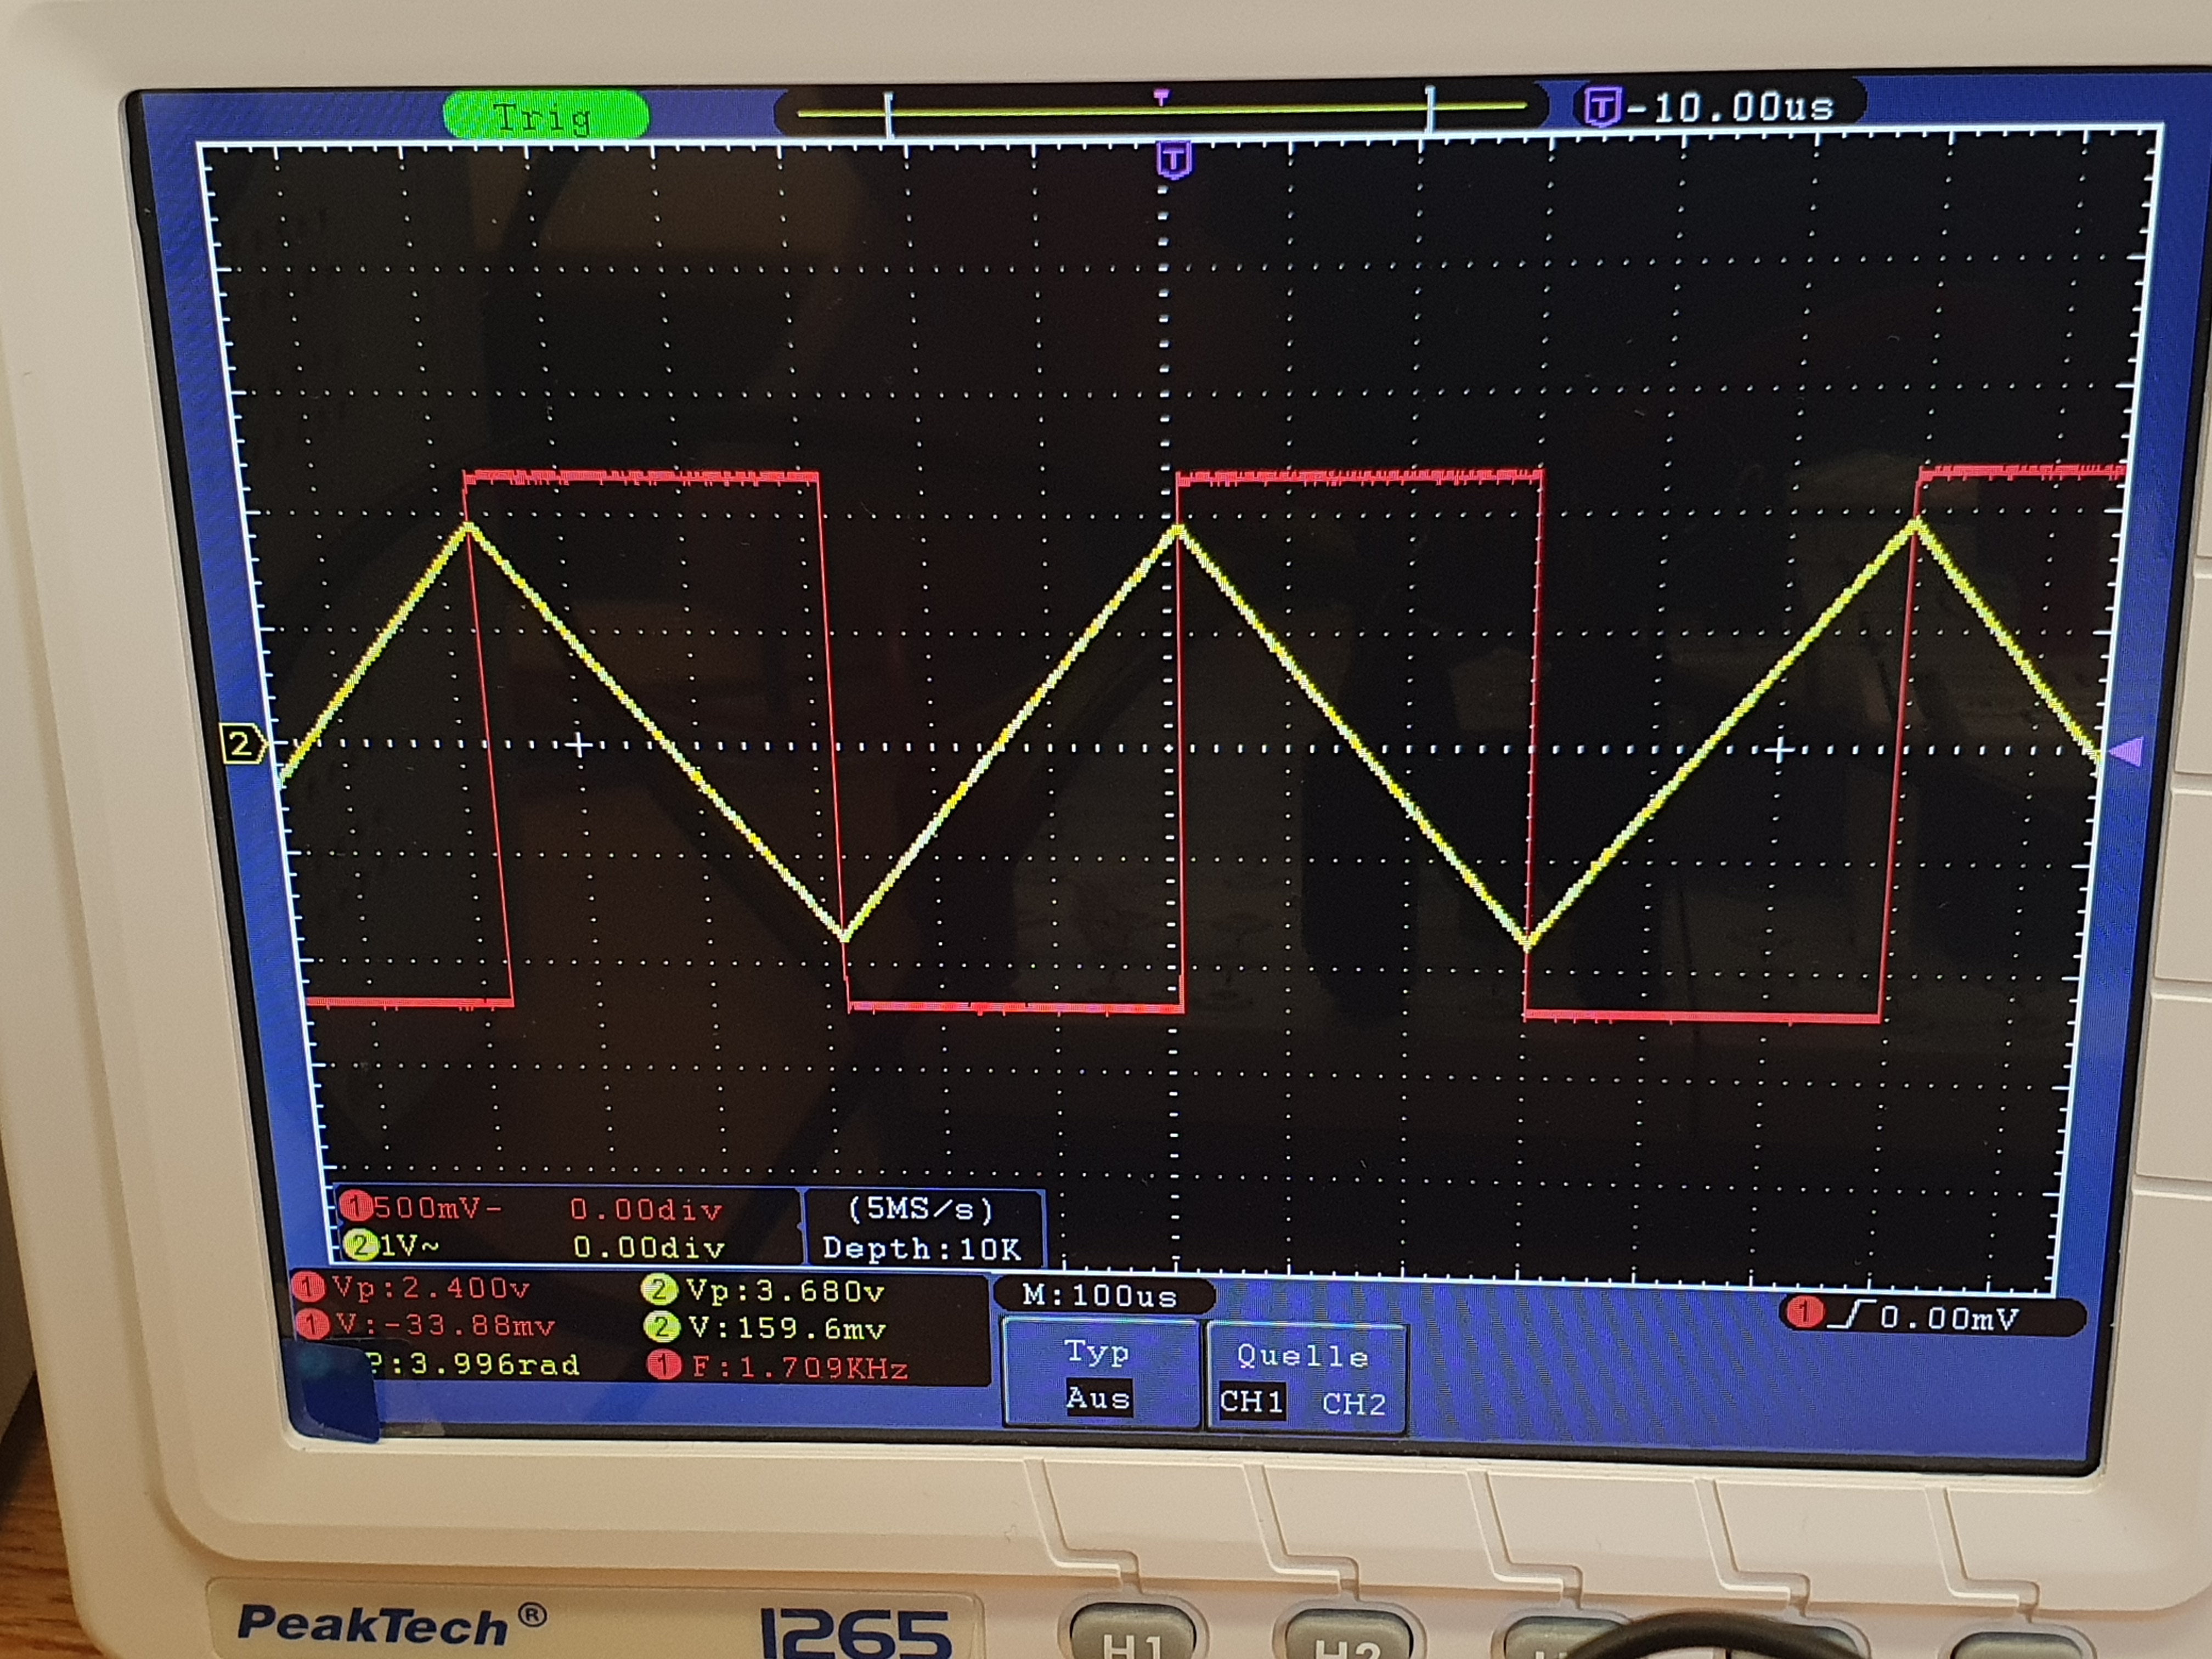
\includegraphics[width=0.4\linewidth]{nudes/messergebnisse/IntegriererRechteck10nF.jpg}
    \caption{Integrierer 10 nF}
    \label{fig:IntegriererResultat1AW}
\end{figure}

\begin{figure}[H]
    \centering
    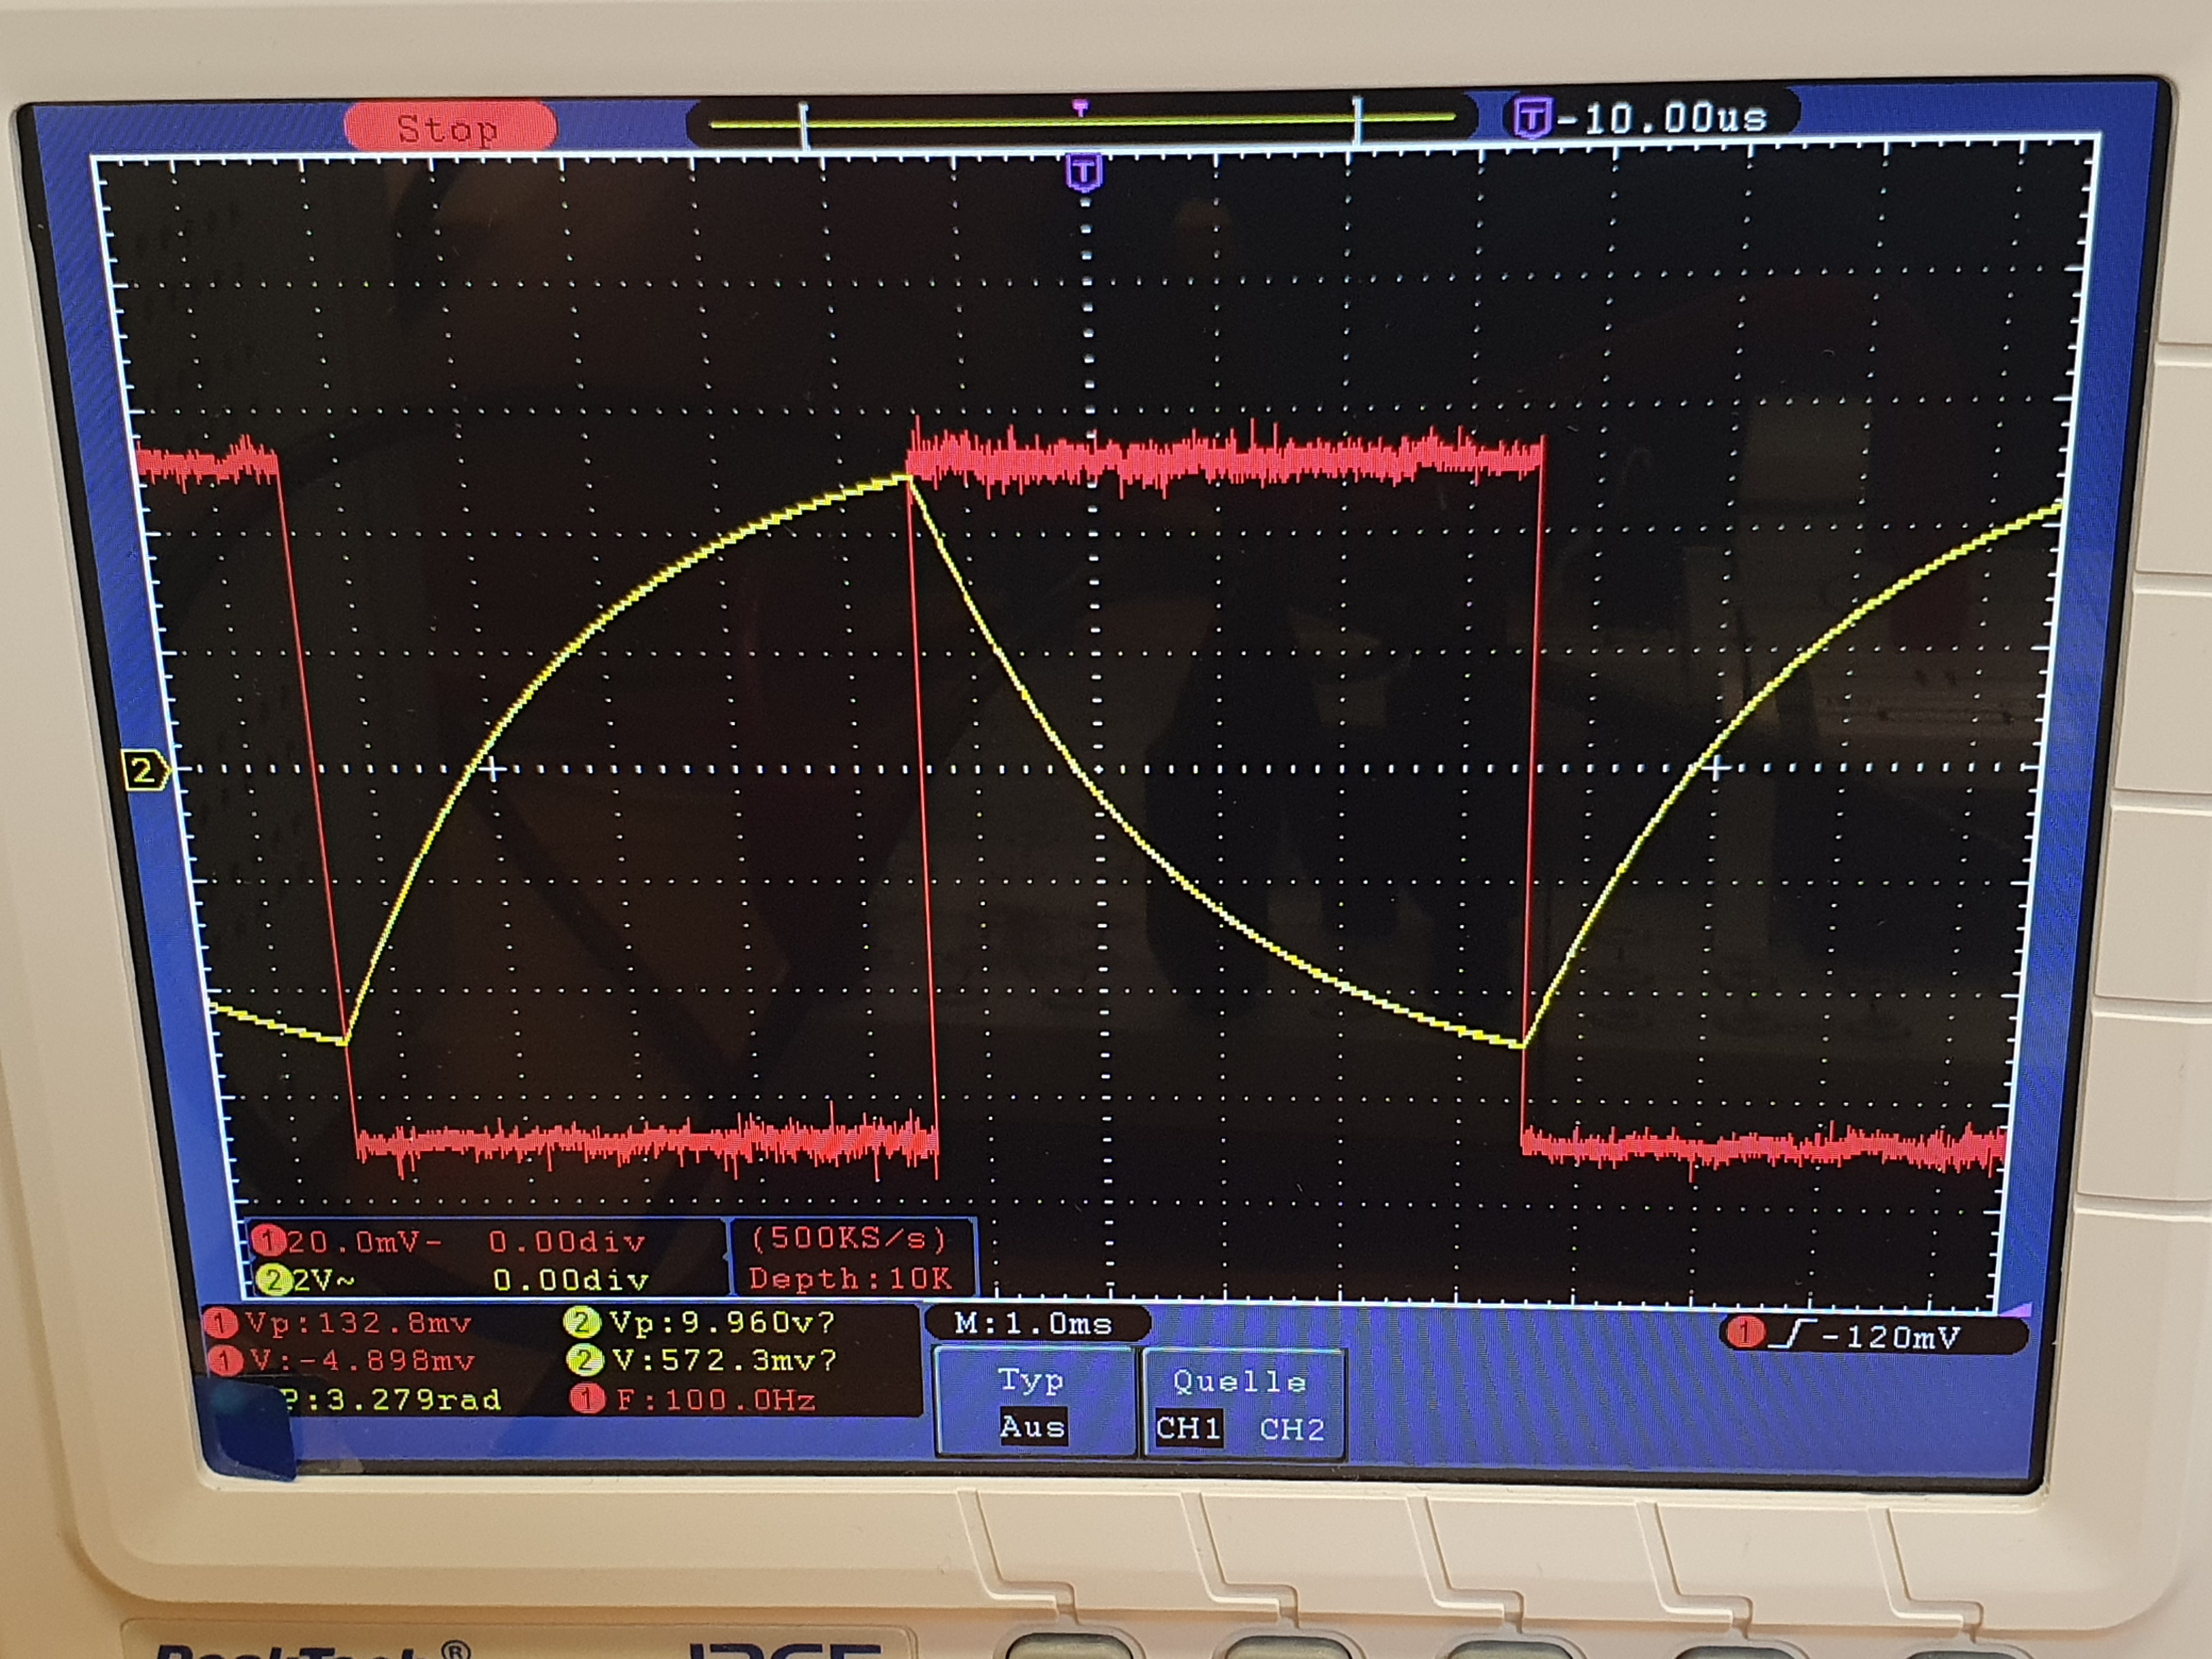
\includegraphics[width=0.4\linewidth]{nudes/messergebnisse/IntegriererRechteck2.2.jpg}
    \caption{Integrierer 2.2 nF}
    \label{fig:IntegriererResultat2AW}
\end{figure}

\begin{figure}[H]
    \centering
    \includegraphics[width=0.4\linewidth]{nudes/messergebnisse/IntegriererSinusResultat.jpg}
    \includegraphics[width=0.4\linewidth]{nudes/messergebnisse/IntegriererDreieckResultat.jpg}
    \caption{Integrierer Sinus/Dreieck}
    \label{fig:IntegriererResultat3AW}
\end{figure}


\section{Anhang}

In diesem Abteil werden die Unsicherheitsrechnungen zur eventuellen Fehlersuche abgebildet. Für Unsicherheiten von Größeren Tabellen wird jeweils die Rechnung des ersten Wertes als Beispiel für die restlichen Größen gezeigt.


\printbibliography[heading=bibintoc]
\end{document}
